\chapter{Experiments}
\label{chapter:experiments}
The solution of this work was validated with a couple of experiments and stress tests. We show in the following, that this approach provides a safe way to avoid collisions with the robot itself as well as avoiding external obstacles. Reviewing the goal statements of the introduction \ref{item:goals}, we conducted the following experiments to get a quantitative evaluation:
\begin{itemize}
	\item Providing a piecewise continuous trajectory of closest point pairs
	\item Avoiding collisions between the actuated hand and external obstacles
	\item Avoiding full self-collision 
\end{itemize}

\section{Robot Hardware Setup}
The conducted experiments have been mainly examined with a real time physics simulator, namely Gazebo. It simulates an appropriate robot behavior in terms of joint position as well as joint velocities.

The full body self-collision avoidance is running successfully on the robot. This being said, this chapter briefly introduces the hardware on the robot (REEM-H in this case) to give the reader an overview over the experiment circumstances. 

REEM-H comprises an embedded computer, running a Ubuntu 12.04 LTS version with a real time kernel. The specifications as they are provided on PAL Robotics website at the time of writing are listed in table \ref{tab:reemhspec}. 

Furthermore, the used robot model is presented below. The three images denote the internals of the robot (figure \ref{fig:reemmodels}). In the first image, we can see the visual model of REEM-H. The kinematic chain is illustrated in the second image. Hereby, the names of the used links are shown as well \footnote{For completeness: We omitted arm\_link\_6 on both arms as they are located in the same position than the tool link. The graphic looks clearer this way and link\_6 carries no necessary need in terms of capsule decomposition.}. In the remainder of this chapter, we may refer to them, as we calculate the closest point pair based on those links. Finally, the third image gives an idea about the undertaken capsule decomposition. 

\begin{figure}[h!]
  \centering
  \subfigure[REEM-H Model]{
  		\label{fig:reemmodel} 
  		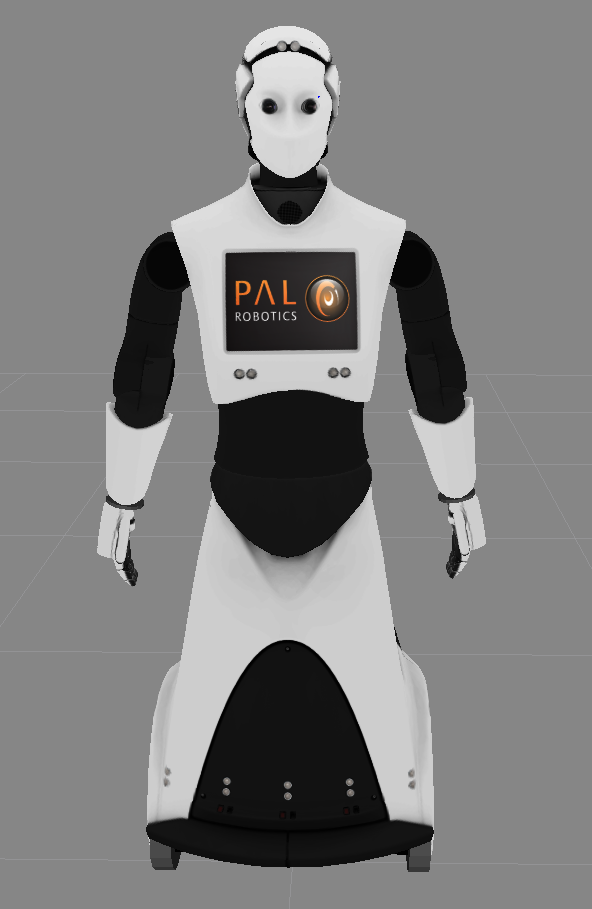
\includegraphics[width=0.3\textwidth]{../figures/reem_model.png}
  	}
  	  \subfigure[Kinematic Chains]{
  		\label{fig:reemtf} 
  		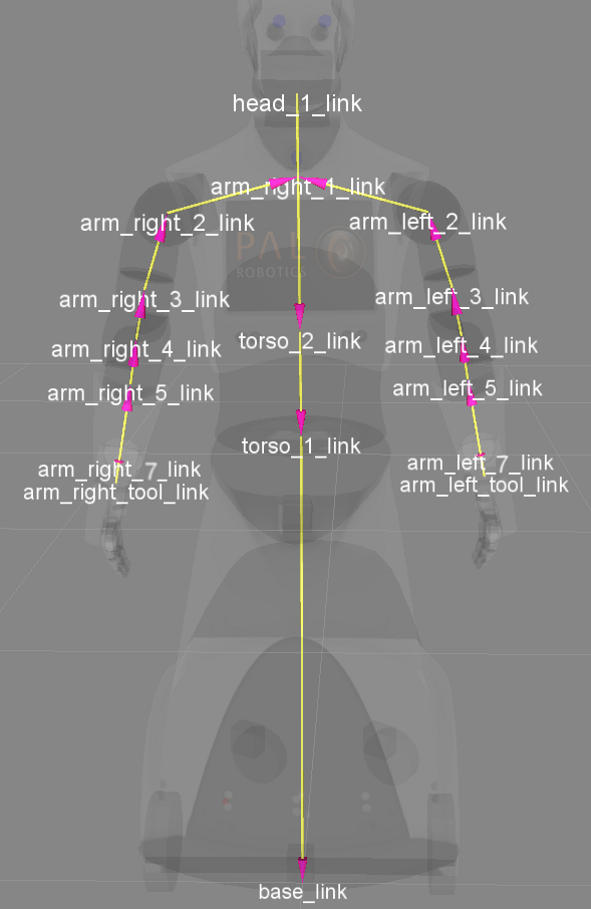
\includegraphics[width=0.3\textwidth]{../figures/reem_model_tf.png}
  	}
  	  \subfigure[Capsule Decomposition]{
  		\label{fig:reemcaps} 
  		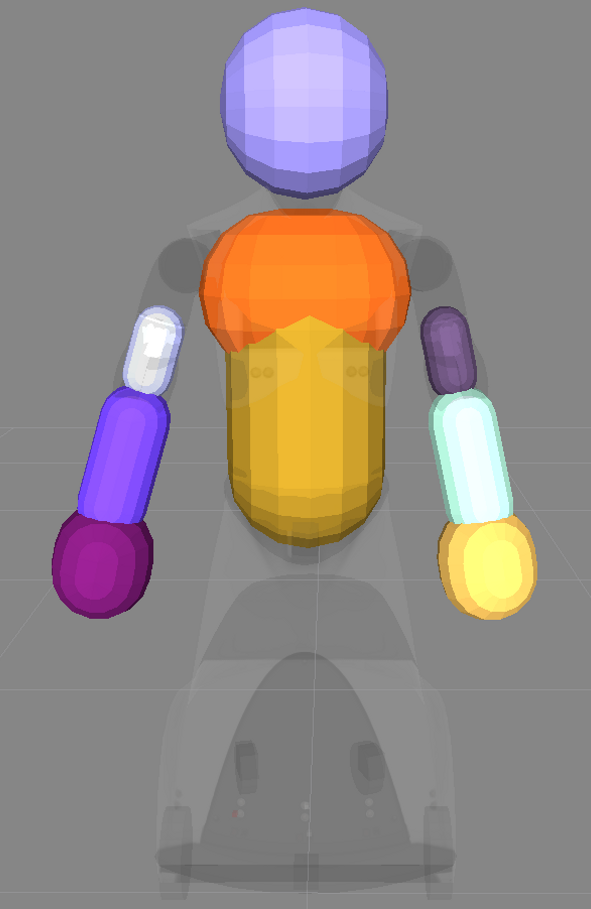
\includegraphics[width=0.3\textwidth]{../figures/reem_model_capsule.png}
  	}
\caption{REEM-H model explained: a) visual surface model. b) kinematic chain of all links. These link names are used as a reference in the remainder of this chapter. c) implemented capsule decomposition. Three capsules are placed on each arm, two on the upper body as well as one for the head.}
    \label{fig:reemmodels}
\end{figure}
During the development of this work, we could determine the shown capsules in figure \ref{fig:reemcaps} as being sufficiently necessary to protect all possible self-collisions. 
Since we are implementing a safety distance threshold on every capsule, the resulting safety padding of all capsules sufficiently covers the left out body parts. Table \ref{tab:capsules} lists the capsule decomposition of the body parts.
\begin{table}[h!]
\parbox{.45\textwidth}{
\begin{tabular}{l l} 
\hline
\multicolumn{2}{ |c| }{REEM-H specification} \\
\hline
weight & 90 KG \\[0.2em]
\hline
height & 1.70 meter \\[0.2em]
\hline
DOF & 22 \\[0.2em]
\hline
Computer & Intel Core2Duo \\[0.2em]
\hline
OS & Ubuntu 12.04 LTS \\[0.2em]
\hline
Kenel & Xenomai real time toolchain\\
\end{tabular}
\caption{Hardware specification of REEM-H}
}\label{tab:reemhspec}
\hfill
\parbox{.45\textwidth}{
\label{tab:capsules} 
\begin{tabular}{l l}
\hline 
\multicolumn{2}{ |c| }{Capsule Decomposition} \\
\hline
\multirow{3}{*}{Right Arm} & arm\_right\_3\_link \\
& arm\_right\_5\_link \\
& arm\_right\_7\_link \\[0.2em]
\hline
\multirow{3}{*}{Left Arm} & arm\_left\_3\_link \\
& arm\_left\_5\_link \\
& arm\_left\_7\_link \\[0.2em]
\hline 
\multirow{2}{*}{Upper Body} & torso\_1\_link \\
& torso\_2\_link \\[0.2em]
\hline
\multirow{1}{*}{Head} & head\_1\_link \\
\end{tabular}
\caption{Capsule Decomposition of REEM-H}
}
\end{table}

\section{Experiments}
All of the following concrete experiments comprise two major tasks. The highest prioritized task of all experiments is joint limit avoidance. This is followed by the task velocity damping introduced in chapter \ref{sec:velocitydamping}, which denotes the (self-)collision avoidance task. Hereby, this is configured according to the respective exercise (such as external collision avoidance or self-collision avoidance). Lastly, the active task for positioning the tool center of the left as well as the right arm is placed at the bottom of the stack. Figure \ref{fig:basicstack} depicts the basic stack used for these experiments. During the experiments, we change the order of the left and right wrist, however they are constantly placed at the bottom of the task.
\begin{figure}[h!]
  \centering
    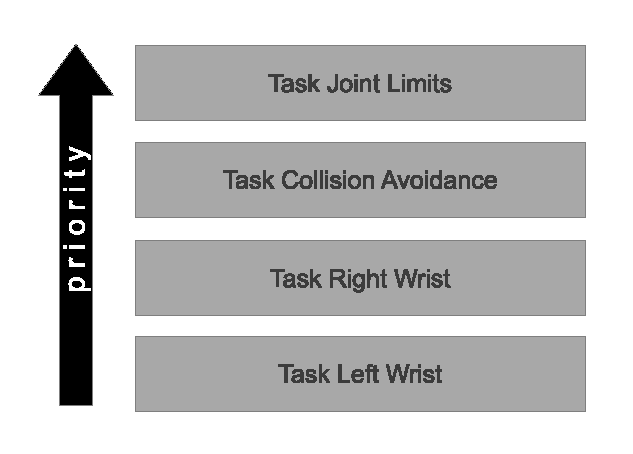
\includegraphics[width=0.4\textwidth]{../figures/stack_experiments.eps}
    \caption{Basic hierarchy stack of used tasks for the experiments. As illustrated, joint limits have always the highest priority. The collision avoidance task takes precedence over the tasks of interest such as the right or left wrist. In the conducted experiments, we will also examine the behavior of changing the order of left and right, yet constantly placing them at least priority.}
    \label{fig:basicstack}
\end{figure}

Beforehand, we implemented two strategies for integrating the SoT inside ROS\_control of the REEM robots. Xenomai respectively ROS\_control operates with a frequency of $100Hz$. This means, that the physical update cycle is lower bounded to $100Hz$ and the computation of the stack has to produce a result with in this cycle. On the same hand, we integrated the SoT as a asynchronous, not real time safe thread, next to ROS\_control. With this decoupling, we can prevent any real time violations to be visible on the robot. This further implies, that we can achieve a higher cycle rate exclusively for the SoT, providing the current solution for every cycle of ROS\_control. 
The purpose of these different cycle rates is essentially the capability of shrinking the $\Delta t$ inside the update cycle of the SoT. We recall the task definition in \ref{eqn:ikleastsquare} again:
\begin{eqnarray}
\vec{\dot{x} = J(q,t) \dot{q}} \notag \\
\vec{\dot{x} = J(q,p)} \frac{\Delta\vec{q}}{\Delta t} \label{eqn:expdeltat}
\end{eqnarray}
From equation \ref{eqn:expdeltat}, it is clear that lowering $\Delta t$ yields to smoother results in $\vec{\dot{x}}$ and thus to a smoother trajectory on the robot. All experiments, which are presented below, were executed with a rate of $100Hz$ inside the SoT, because of limits in computation power of the embedded computer inside REEM.

\subsection{Continuous Trajectory of Closest Points}
In chapter \ref{sec:closestpoints}, we examined the benefit of exercising a capsule decomposition over a mesh collision geometry. The goal in this experiment is to demonstrate the required continuity of the closest point pair. Informally spoken, monitoring the trajectory of each point of the according point pair must result in one single path and is not allowed to jump in position. 

For this experiment, we move the right arm from the right ($x:-0.2m,y:-0.3m,z:1.1m$) to the left($x:0.2m,y:0.3m,z:1.1m$). Hereby, we examine the development of the closest point pair between arm\_right\_5\_link and the Upper Body as well as Head. The arm movement as well as the closest point calculation is shown in the two figures below (figure \ref{fig:cpexperiment}). Figure \ref{fig:cplines} contains information about the closest point pairs at time $t_k$ for a specific $k$. The lines mark the connection between the two points which form a collision pair. 

\begin{figure}[h!]
  \centering
  \subfigure[Executed trajectory]{
  		\label{fig:cptraj} 
  		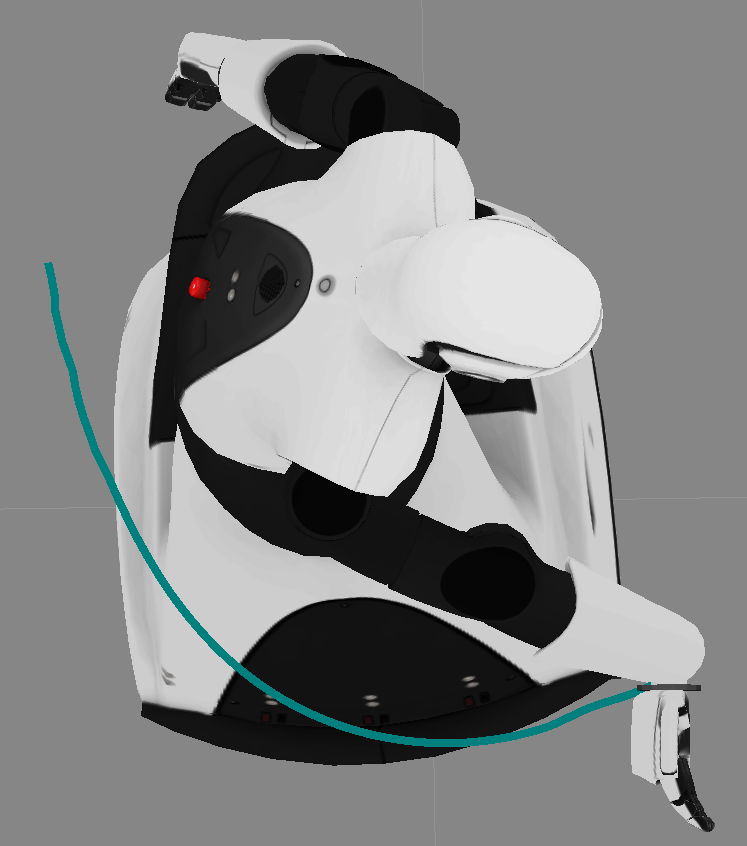
\includegraphics[width=0.35\textwidth]{../figures/closest_points/robot_path.png}
  	}
  	  \subfigure[Closest Point Pairs]{
  		\label{fig:cplines} 
  		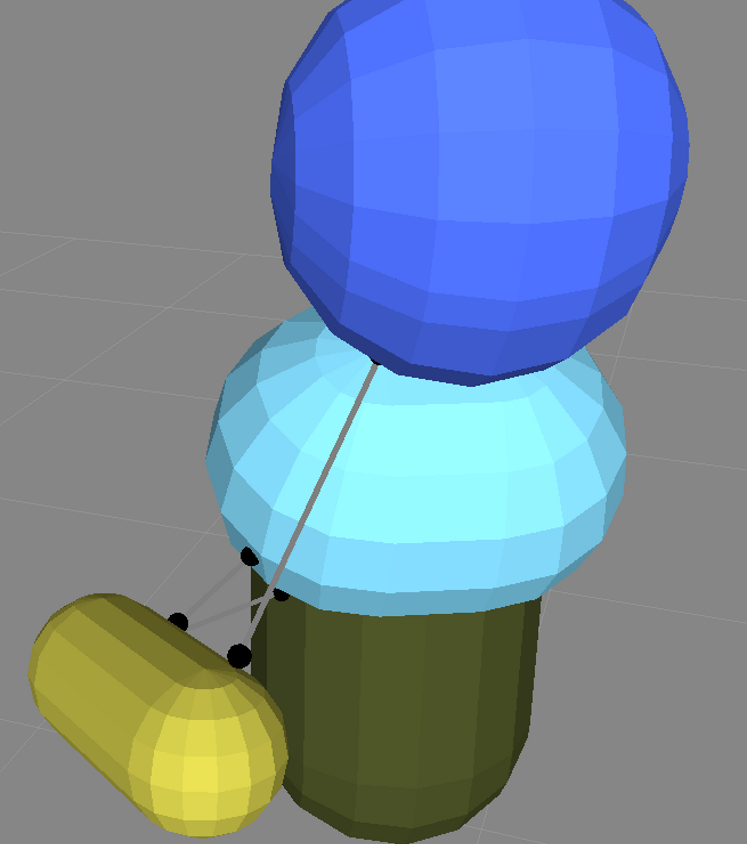
\includegraphics[width=0.35\textwidth]{../figures/closest_points/lines.png}
  	}
\caption{Closest Point Trajectory: a) shows the trajectory the right arm executed. The robot moved around the torso from the right ($x:-0.2m,y:-0.3m,z:1.1m$) to the left($x:0.2m,y:0.3m,z:1.1m$) (seen from the robot perspective). b) denotes the closest point pairs between the three collision pairs at $t_k$. The development of this calculation has to be continuous for all $t_i$. The lines are providing info which points belong to which collision pair.  } 
    \label{fig:cpexperiment}
\end{figure}

The result of this particular experiment is exposed below. We can see in the results (figure \ref{fig:cptogether}), that the requirement is fulfilled as the trajectory for all closest points is continuous. The plots show the path in $x$ and $y$, since the executed movement is planer in $z:1.1m$. The left plot describes the points, which are attached at the \verb|arm_right_5_link|. Their data is expressed with respect to the global base frame. Equally, the right plot represents the points on the Upper Body and Head.
%\begin{figure}[h!]
%  \centering
%  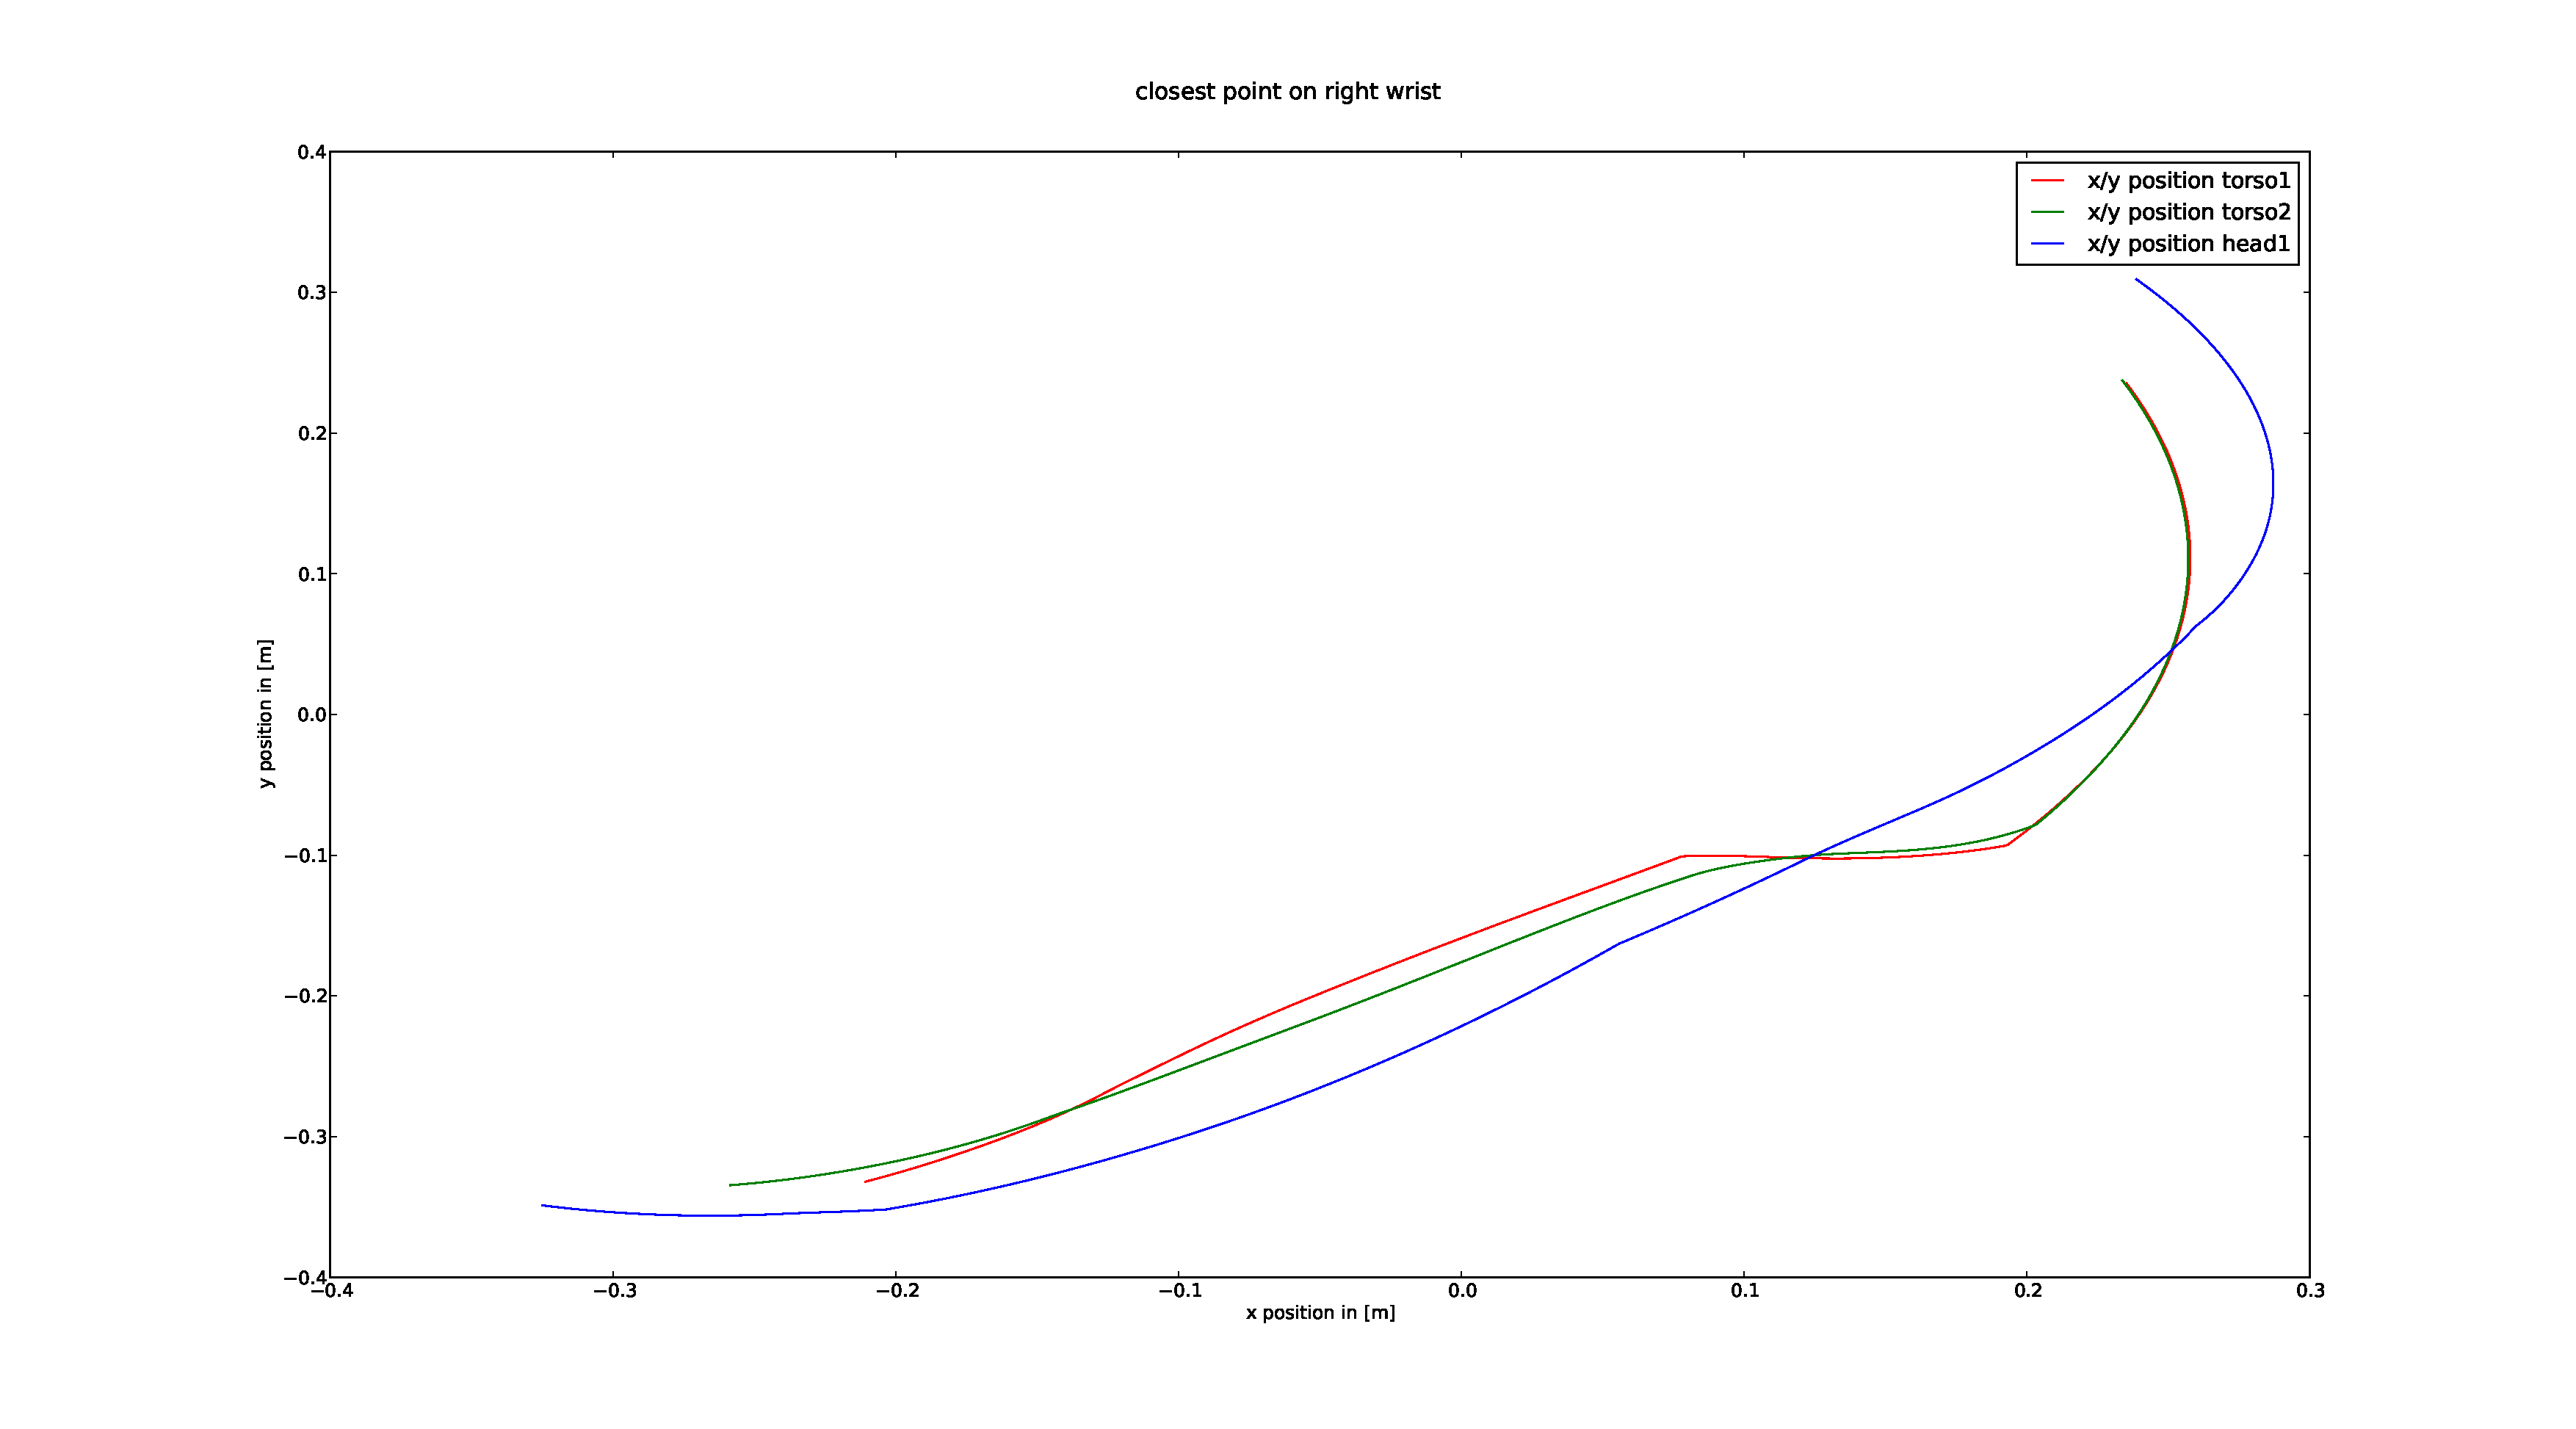
\includegraphics[width=0.9\textwidth]{../figures/closest_points/three_topics_rw.eps}
%\caption{closest point development of the points lying on \texttt{arm\_right\_5\_link}. The result is a continuous path, which illustrates a correct behavior of the calculation.} 
%    \label{fig:cprw}
%\end{figure}
%\begin{figure}[h!]
%  \centering
%  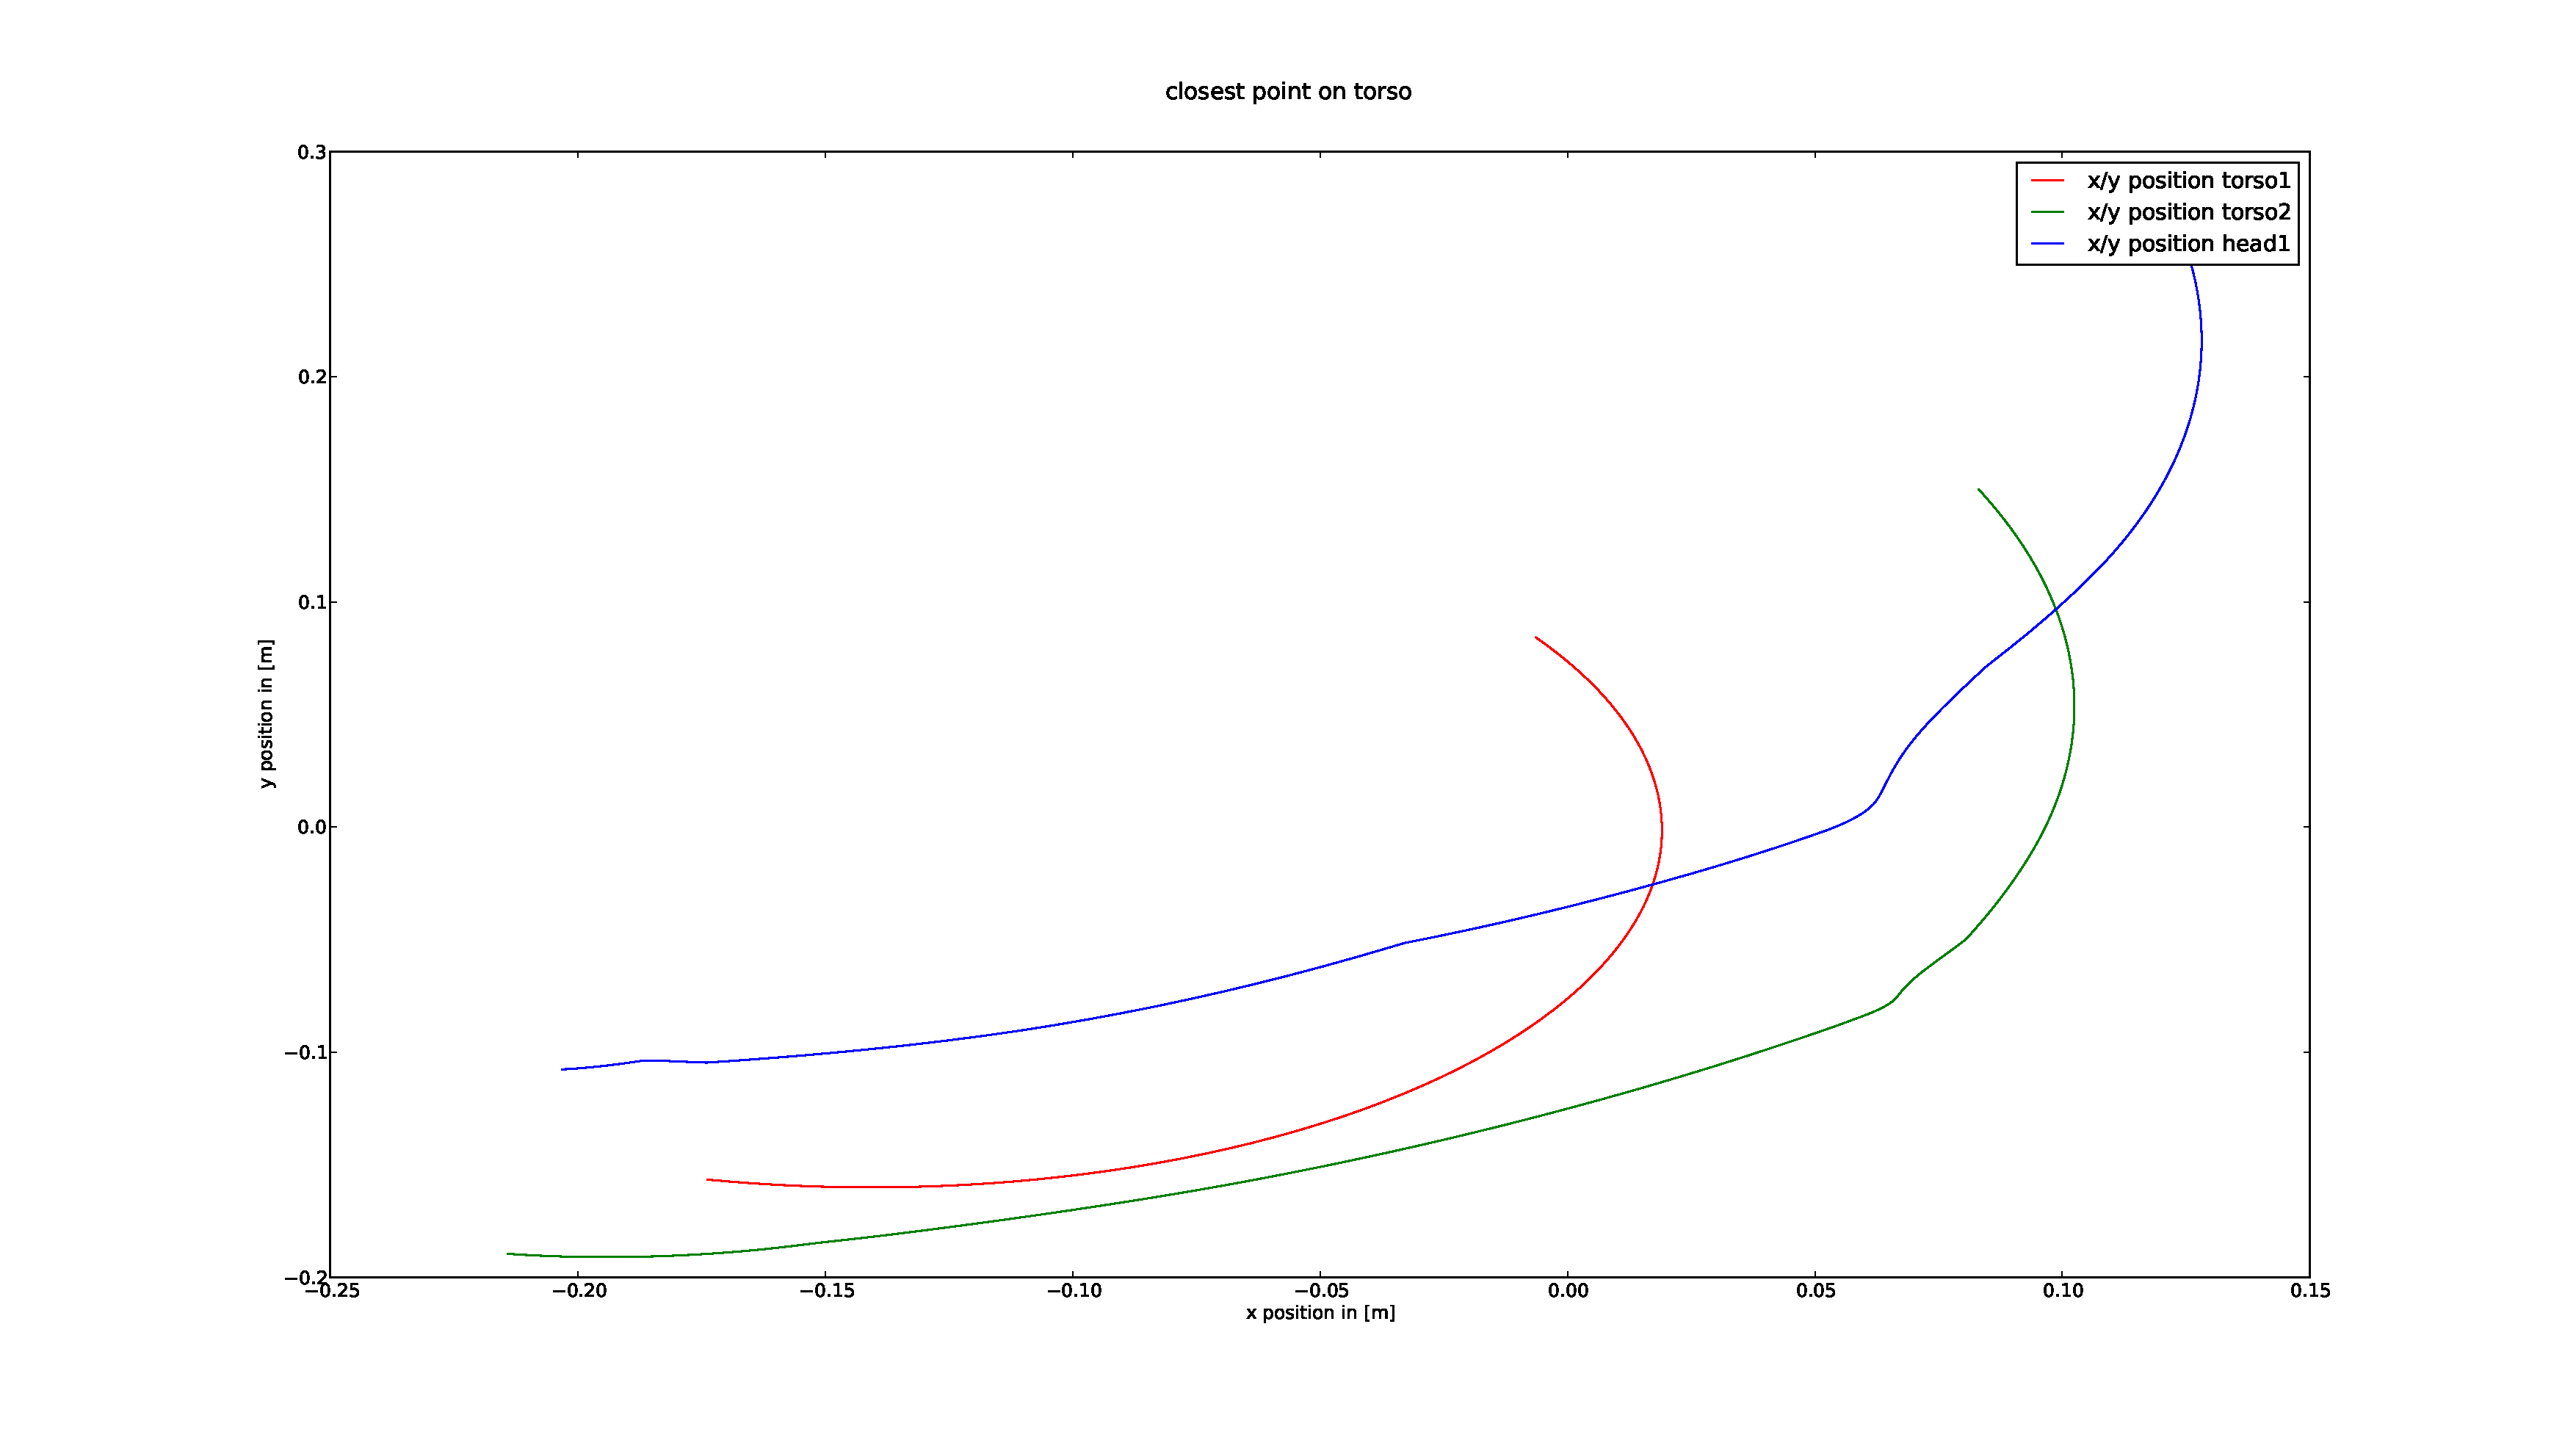
\includegraphics[width=0.9\textwidth]{../figures/closest_points/three_topics_torso.eps}
%\caption{closest point development of the points lying on Upper Body and Head, respectively. The result is also continuous path, which illustrates a correct behavior of the calculation.} 
%    \label{fig:cptorso}
%\end{figure}
\begin{figure}[h!]
  %\centering
  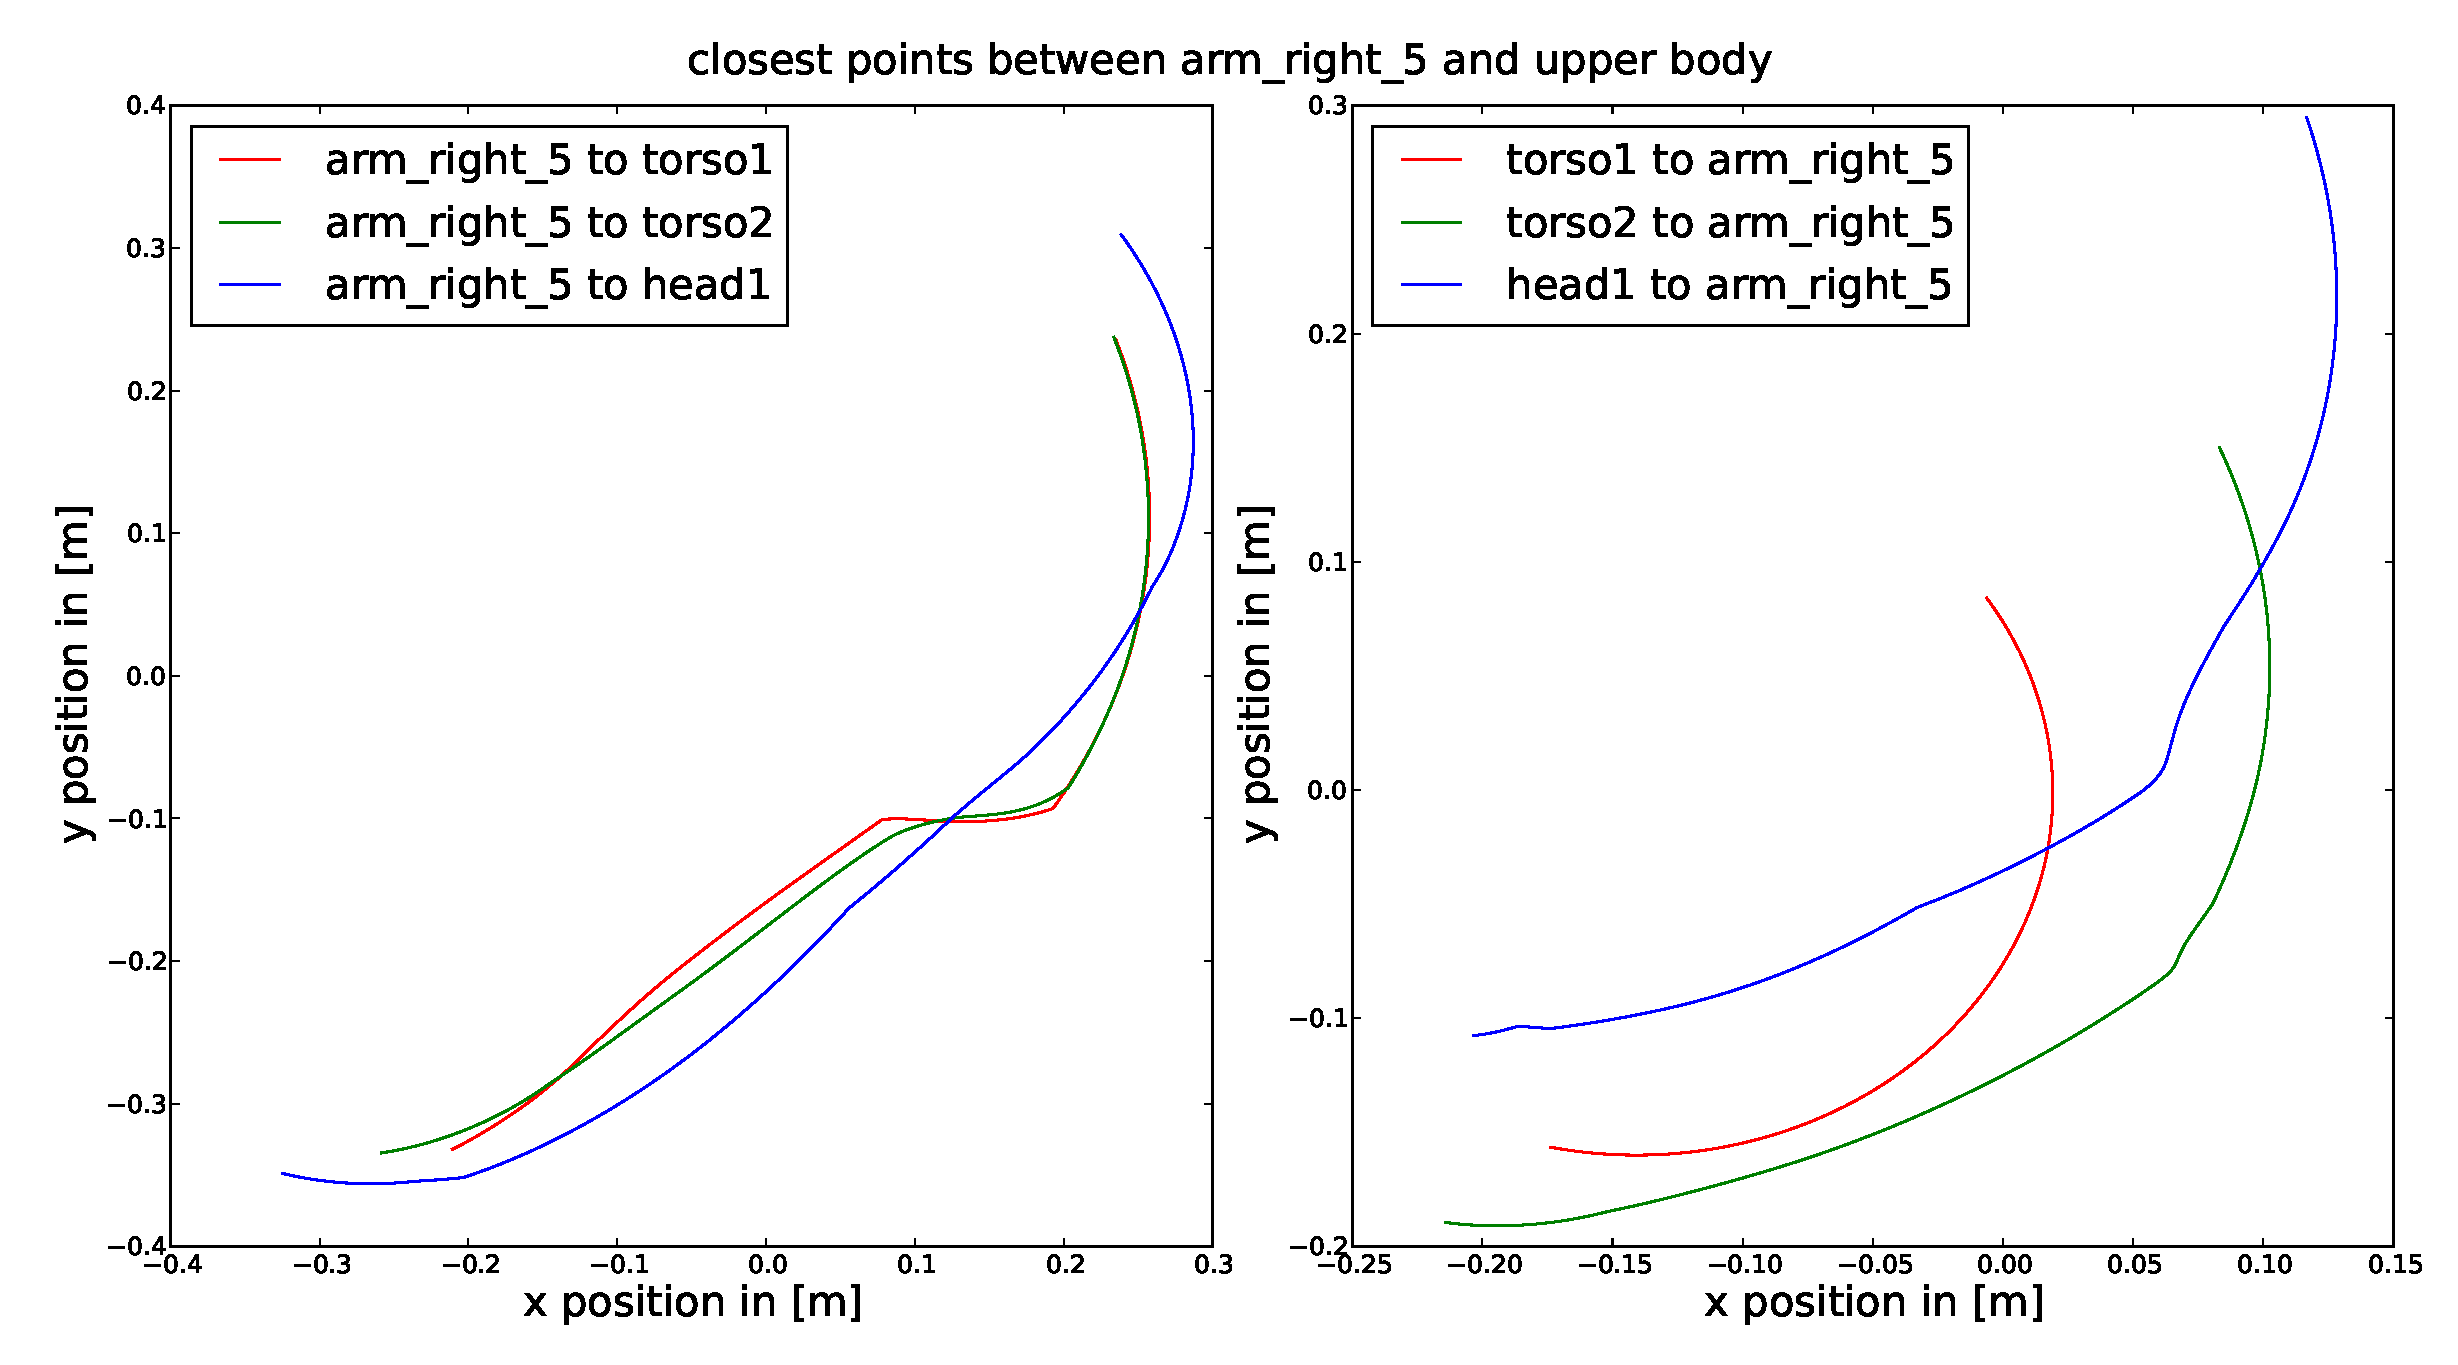
\includegraphics[width=\textwidth]{../figures/closest_points/three_topics_together.eps}
\caption{closest point development between \texttt{arm\_right\_5\_link} and Upper Body (consisting of \texttt{torso\_1, torso\_2, head\_1}). Left diagram shows the closest points lying on the capsule of the right arm towards the upper body. Similarly, the right diagrams displays the counter points on the upper body, which are pointing towards the right arm. } 
    \label{fig:cptogether}
\end{figure}

This experiment was successfully executed with all possible collision pairs with similar results. We encounter a rather negative result, when joint limits or clamping situations occur as the resulting joint velocities might increase dramatically. This inevitably leads to a high displacement of the closest points.
\clearpage
\newpage
\newpage
\subsection{External Collision Avoidance}
To begin with, we conduct the experiment of avoiding external obstacles coming across a predefined trajectory of one of the arms. Hereby, we specify a trajectory input signal inside the dynamic graph, which provides the desired position of the right tool joint. Equally, we specify a similar signal representing the obstacle position. Thus, we have to configure the closest point pair $p_1$ as the right wrist signal and the $p_2$ as the obstacle signal. 

\subsubsection*{Static Object vs. Moving Arm}
The first experiment describes a statically placed collision obstacle. The right wrist has to avoid this obstacle, yet minimizing the error between the actual and desired position to the best. The task specifying the left wrist position is not on the stack in this experiment. The predefined trajectory denotes a path from the left to the right and is shown in the following sequence of screen shots \ref{fig:externarmmoves}. The control gain $\epsilon$ for the velocity damping task is set to $1$, $d_s$ is set to $0.1m$. The control gain $k$ for the right wrist task is set to $10$. 
\begin{figure}[h!]
  \centering
  \subfigure[]{
  		\label{fig:armmoves1} 
  		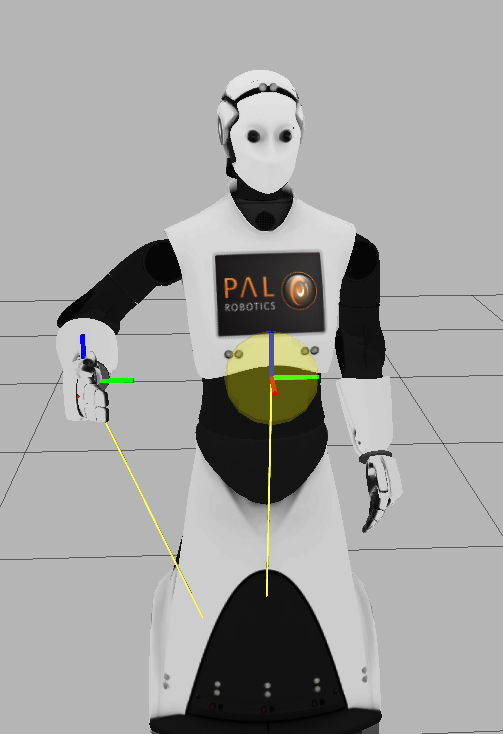
\includegraphics[width=0.23\textwidth]{../figures/arm_moves/1.png}
  	}
  	  \subfigure[]{
  		\label{fig:armmoves2} 
  		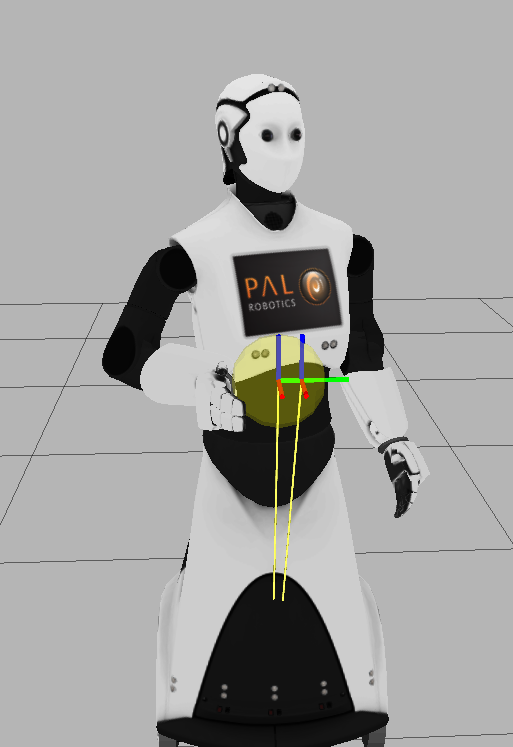
\includegraphics[width=0.23\textwidth]{../figures/arm_moves/2.png}
  	}
  	  \subfigure[]{
  		\label{fig:armmoves3} 
  		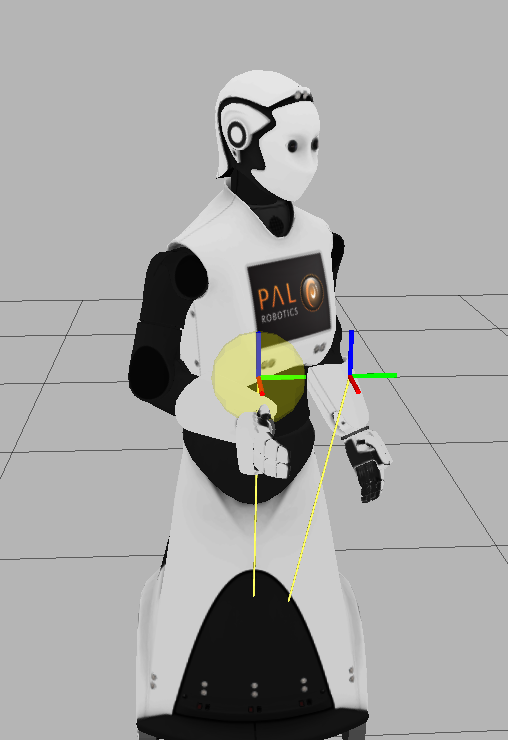
\includegraphics[width=0.23\textwidth]{../figures/arm_moves/3.png}
  	}
  	  \subfigure[]{
  		\label{fig:armmoves4} 
  		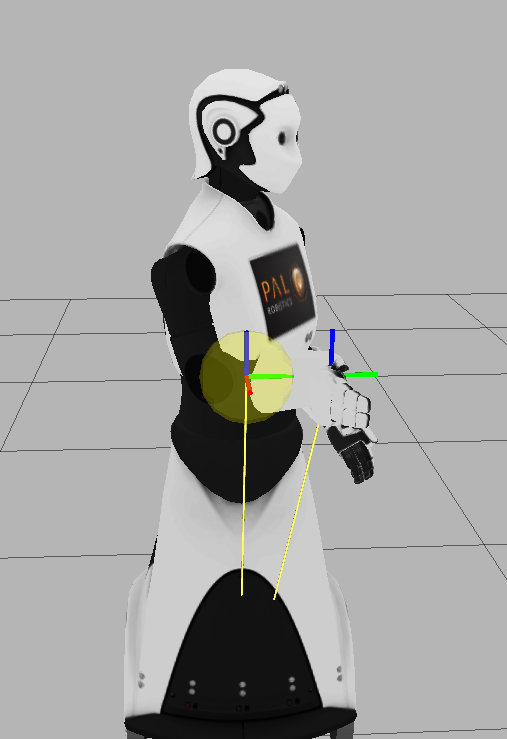
\includegraphics[width=0.23\textwidth]{../figures/arm_moves/4.png}
  	}
\caption{Sequence of screen shots for the predefined trajectory. The yellow ball represents the external obstacle, which has to be avoided. a) starting position b) collision avoidance gets activated as the obstacle boundary is reached c) alternate trajectory trying to minimize the error d) reaching desired position and collision avoidance is deactivated.}
    \label{fig:externarmmoves}
\end{figure}
In the sequence of screen shots, we can see that the arm is following the trajectory until the collision object is reached. At this point the collision avoidance task becomes part of the active set and the movement along the directional vector is limited. In order to minimize the error, an alternative path is solved and the obstacle is avoided.
A closer look at the trajectory is provided in figure \ref{fig:resultexternal}. It is remarkable, that the solver computes a different solution for the way back. Reasons for this might be the different starting configuration, where the HCOD fosters different joint movements at different times.
\begin{figure}[h!]
  \centering
    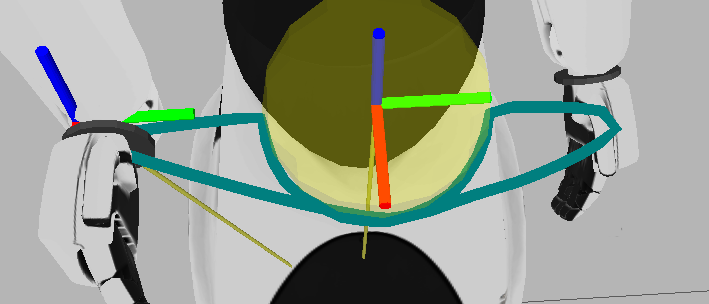
\includegraphics[width=0.6\textwidth]{../figures/arm_moves/result.png}
    \caption{Avoidance of external obstacle. In order to avoid the obstacle, yet minimizing the error towards the goal position, the movement yields along the collision object. The trajectory computed for the way back differs from the initial way. Reason for this are different starting positions and conditions. The HCOD solves the resulting equation system differently and fosters joint movements, which vary from the initial solution.}
    \label{fig:resultexternal}
\end{figure}

The distance over time is depicted in the plot below (Figure \ref{fig:externaldist}). Within this, we can see that the critical distance threshold $d_s$ is set to $0.1m$, which will not be violated. The distance between the obstacle and the wrist stays constantly over this specific safety zone.
\begin{figure}[h!]
  \centering
    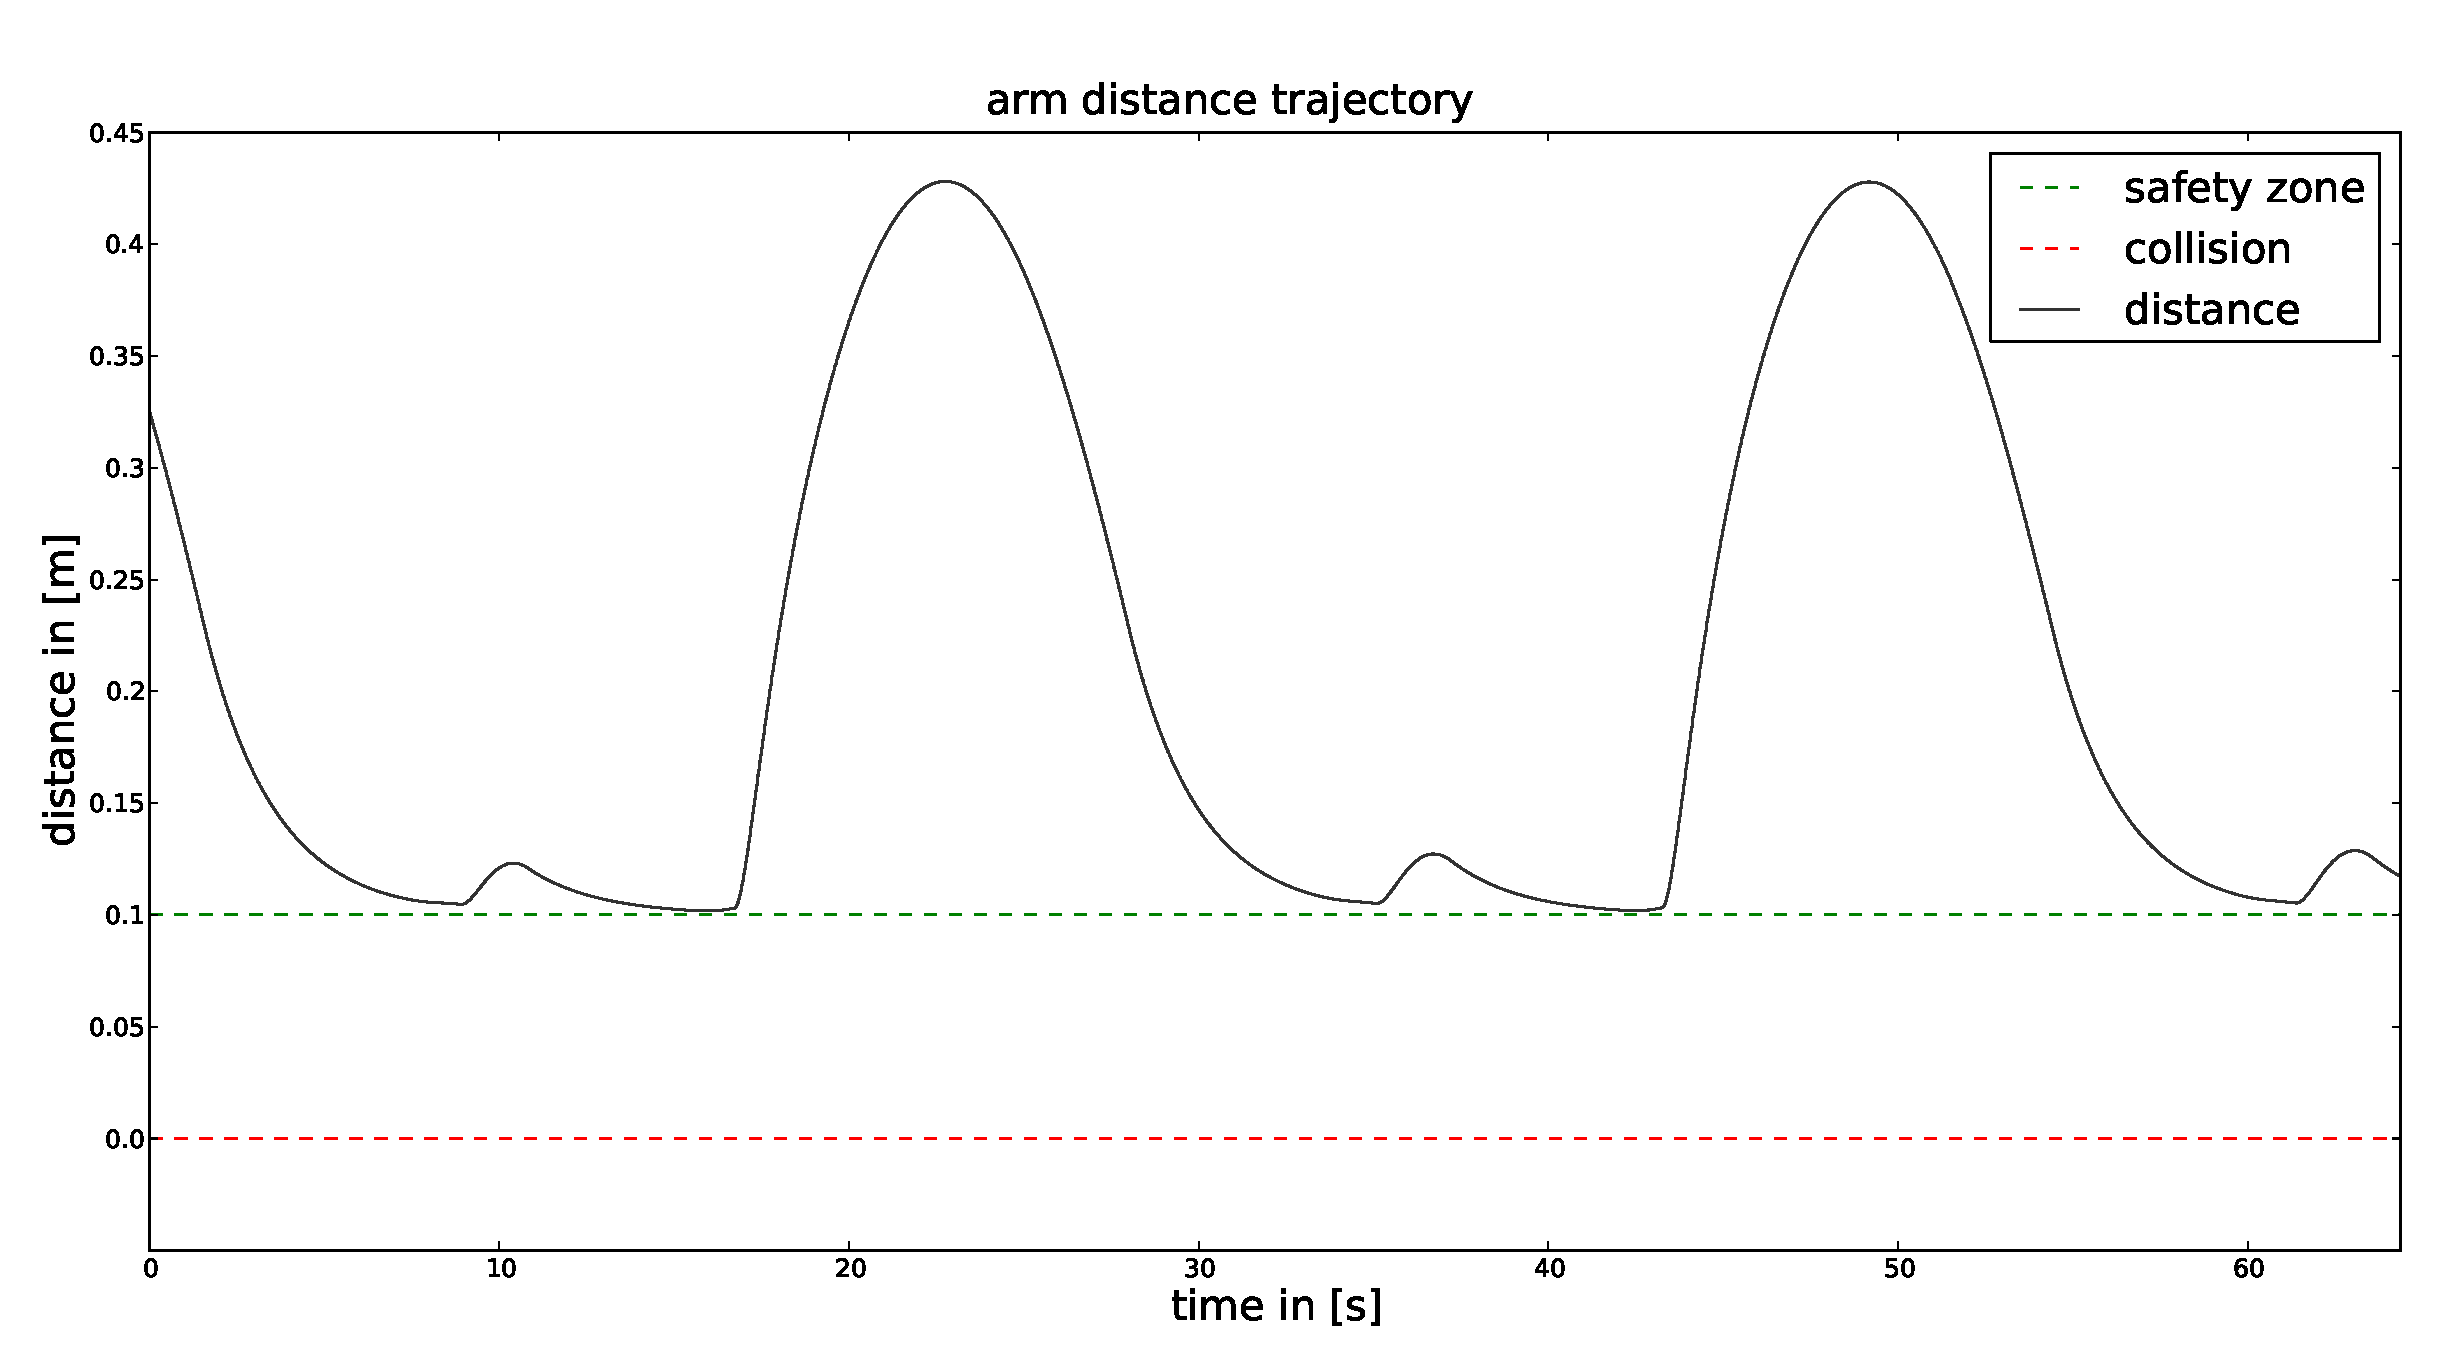
\includegraphics[width=\textwidth]{../figures/arm_moves/distance.eps}
    \caption{Distance plot over time. The distance stays constantly over the safety zone, which is specified as $0.1m$. The red line indicates a distance of 0, which is obviously the result of a full contact collision.}
    \label{fig:externaldist}
\end{figure}
When we look at the position trajectory in figure \ref{fig:externalposition}, we can also see the expected result. The displacement of the actual wrist position, compared to the desired position increases, when the distance converges towards the lower boundary. Furthermore, we can clearly see the attempt of the numerical solver to minimize the error to its best using non-constrained DOF. We can see this behavior around time $t=10s$. Since the desired trajectory is a sine wave in $Y$, the direction along this axis gets constrained, when the wrist moves closer to the obstacle. It can be seen, that the two DOF, such as $X$ and $Z$ are not constrained and can be used to minimize the error. We can see this in the plot, whenever there is an error value in $X$ and $Z$. 
\begin{figure}[h!]
  \centering
    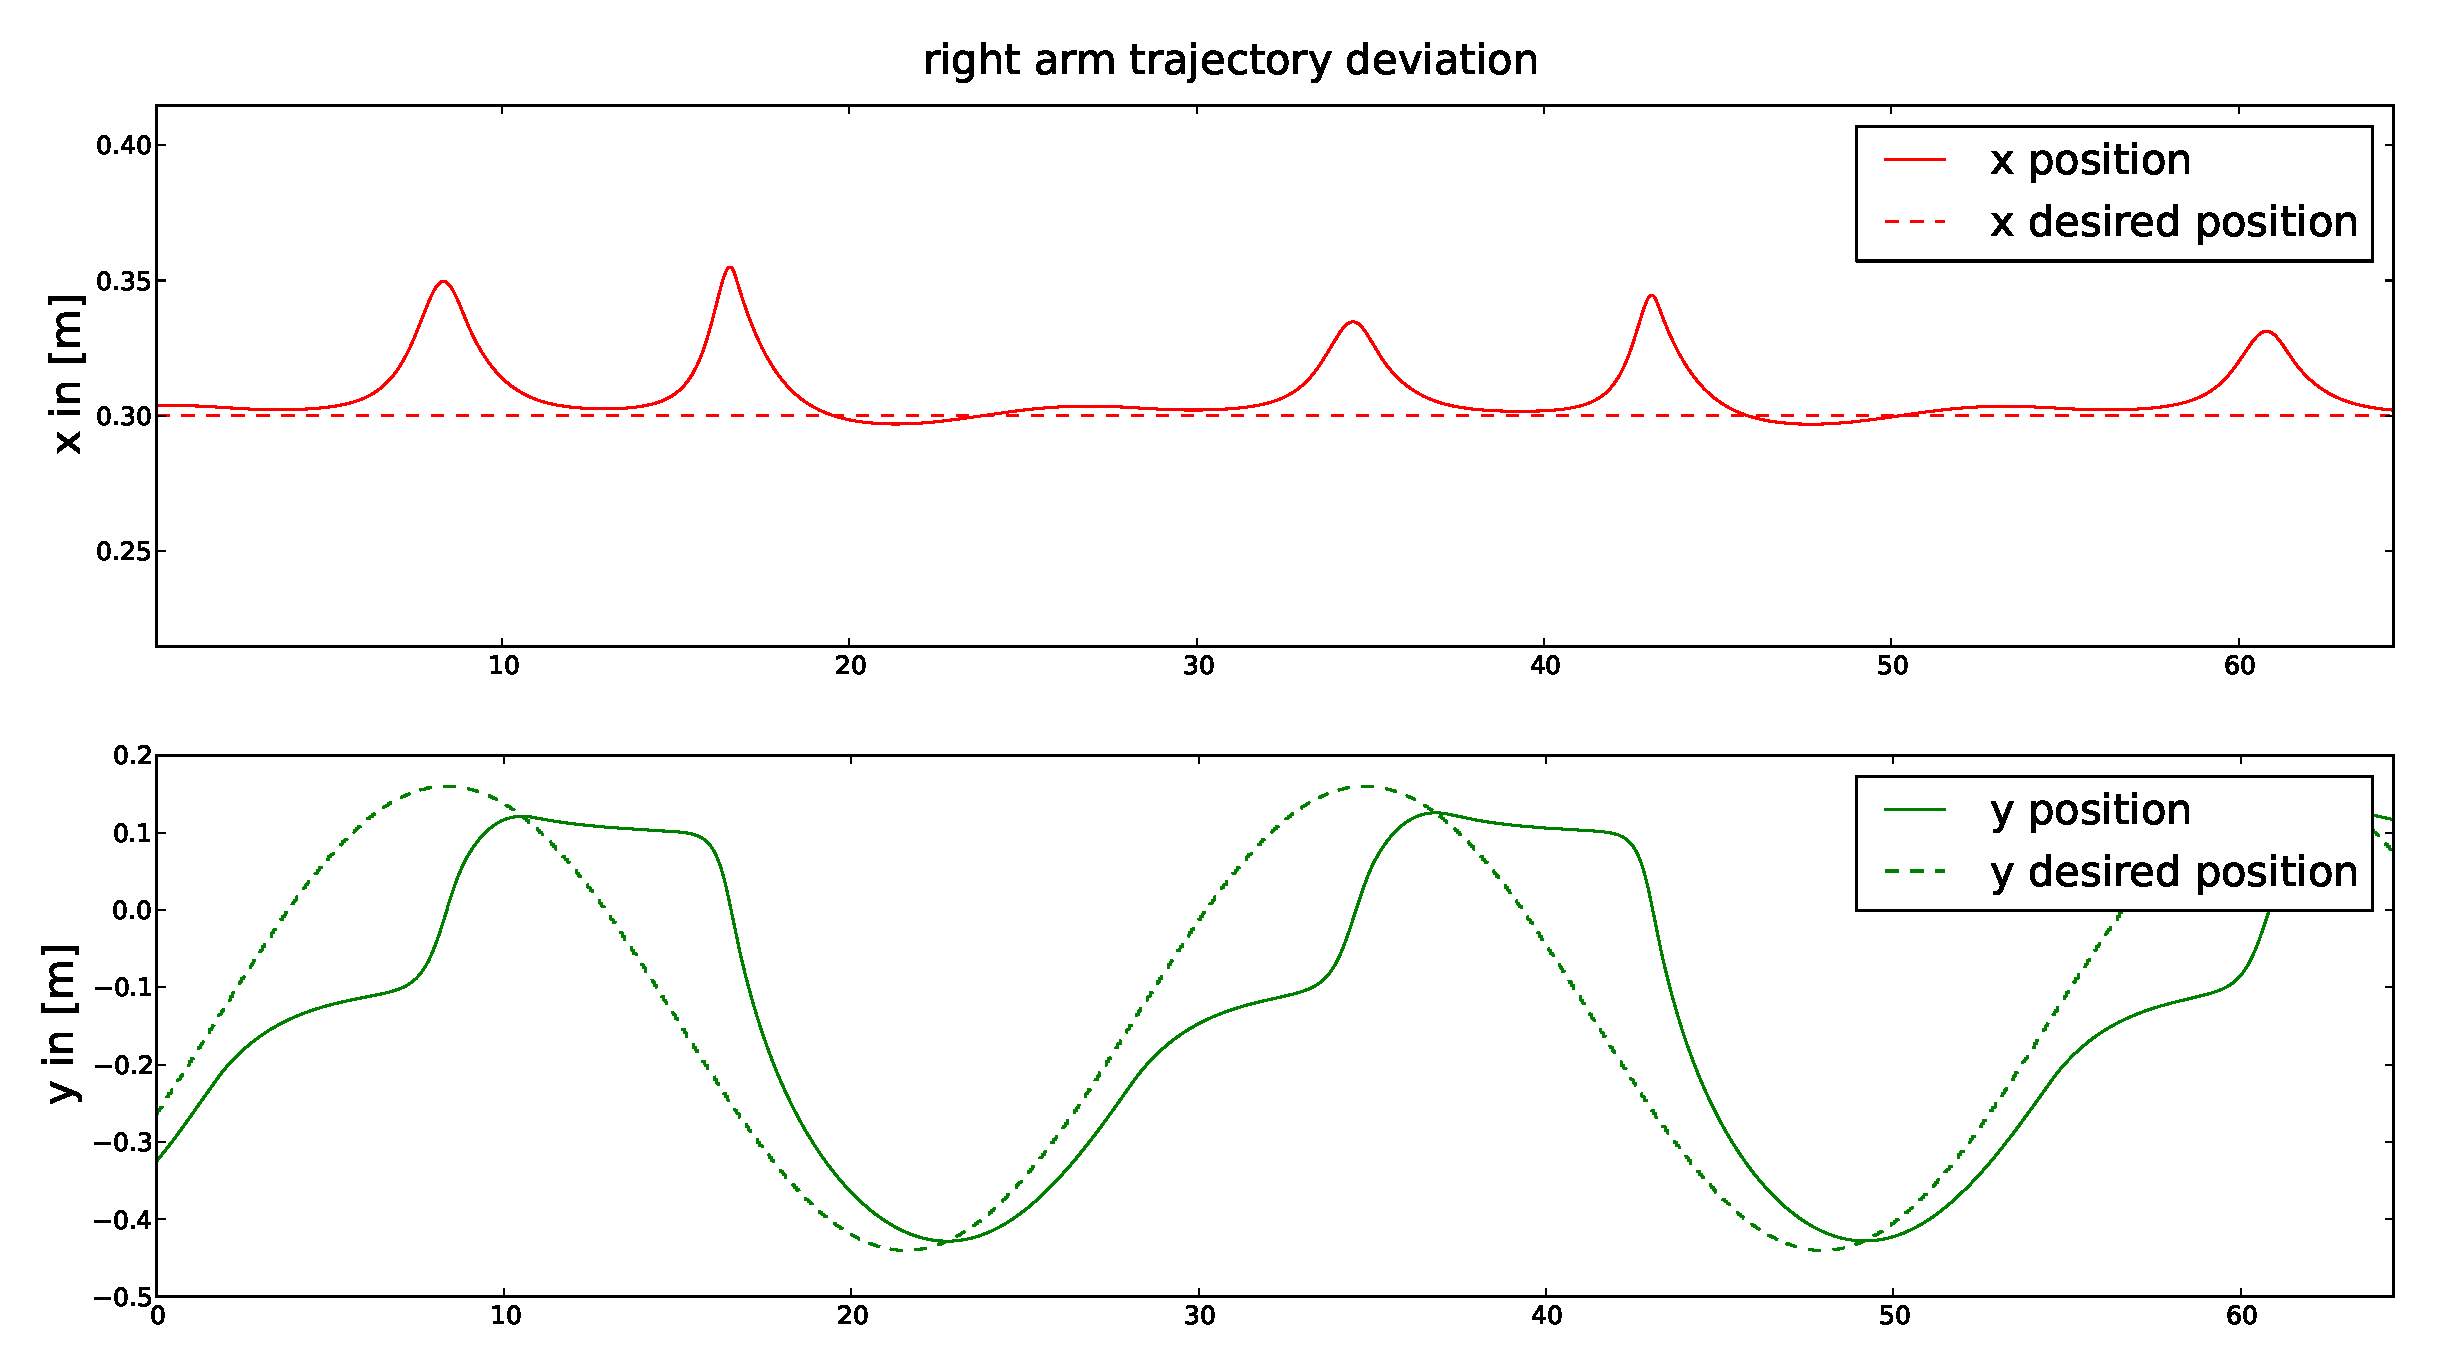
\includegraphics[width=\textwidth]{../figures/arm_moves/position1.eps}
    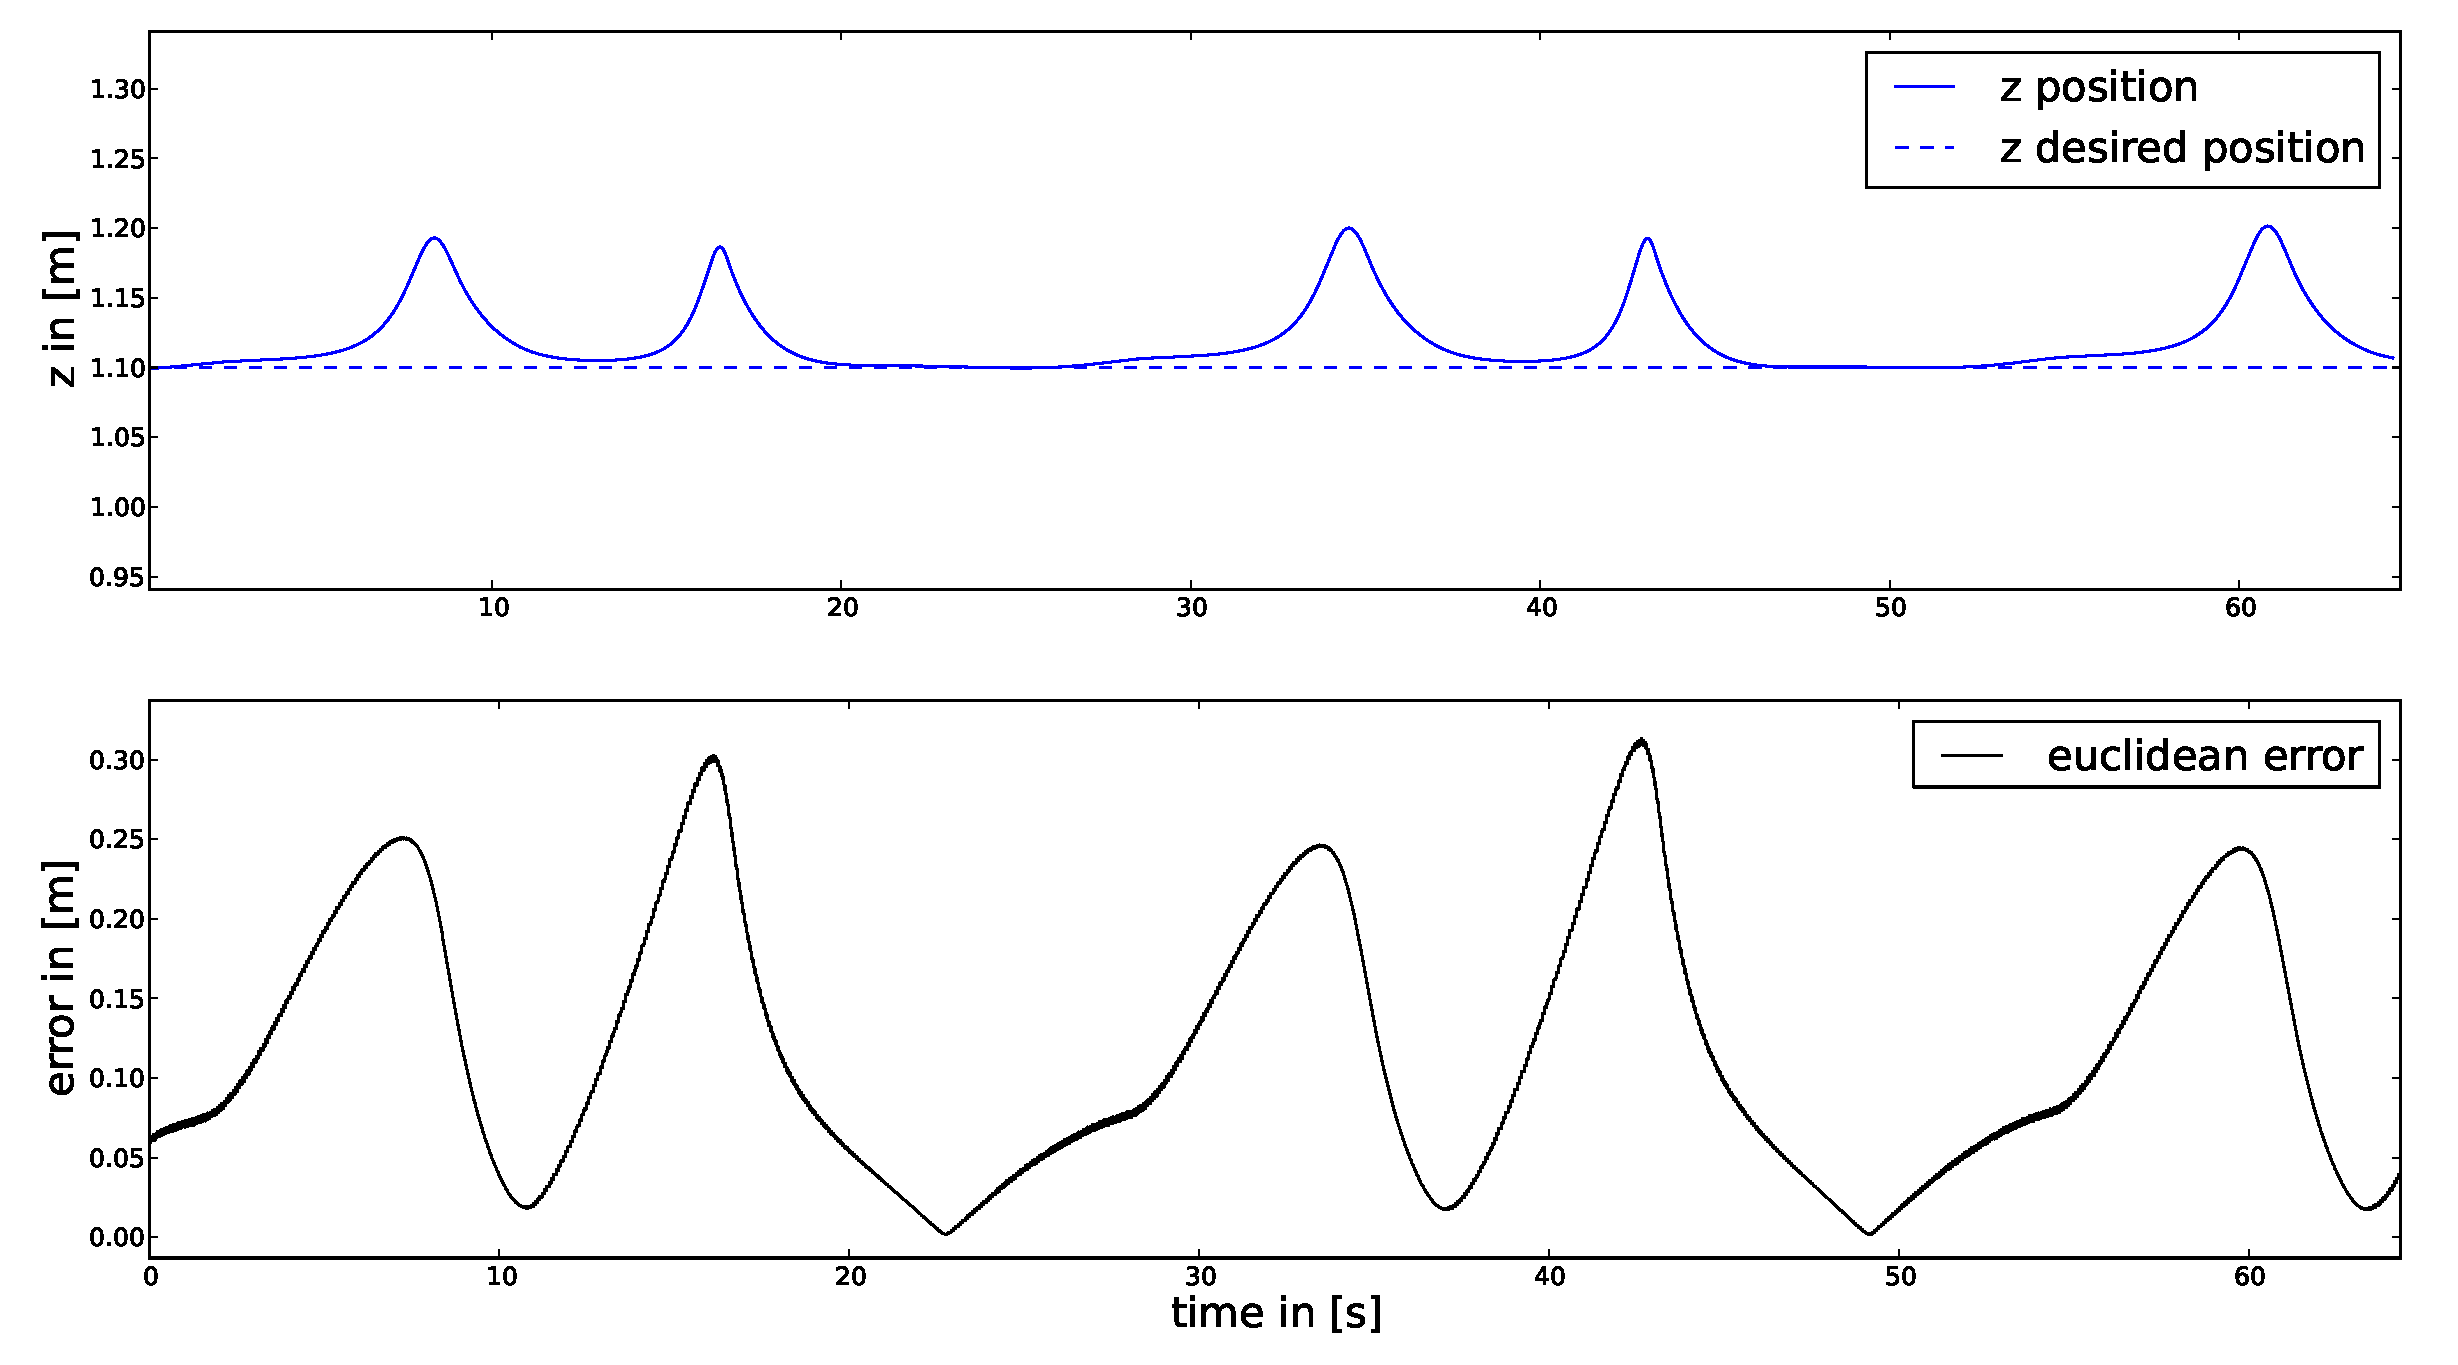
\includegraphics[width=\textwidth]{../figures/arm_moves/position2.eps}
    \caption{Position plot over time. Once a collision boundary is reached, the error increases as long as the obstacle constraint. Once the obstacle got avoided, the errors minimizes again as the goal position can be reached.}
    \label{fig:externalposition}
\end{figure}
\clearpage

\subsubsection*{Moving Object vs. Static Arm}
In the previous experiment, we moved the arm along a predefined trajectory, whereas the object was at a fixed position. In this experiment, we analyze the contrary setup. In the following, we keep the wrist at a static position and move the obstacle along a path, which would finally lead to a collision. We configured the velocity damping with a $\epsilon=10$. Equal to the previous test, $k$ was set to $10$ for the positioning task. Again, the executed trajectory is illustrated in the following sequence of graphics (figure \ref{fig:externobjectmoves}).
\begin{figure}[h!]
  \centering
  \subfigure[]{
  		\label{fig:objmoves1} 
  		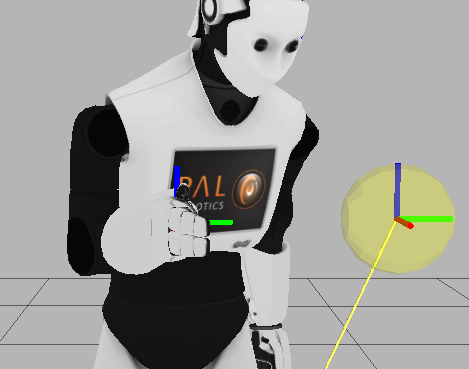
\includegraphics[width=0.23\textwidth]{../figures/object_moves/1.png}
  	}
  	  \subfigure[]{
  		\label{fig:objmoves2} 
  		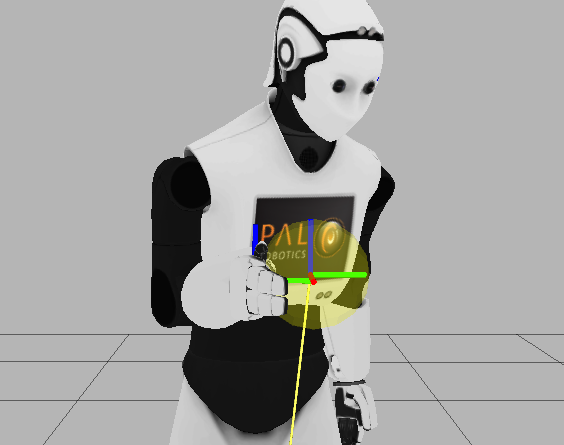
\includegraphics[width=0.23\textwidth]{../figures/object_moves/2.png}
  	}
  	  \subfigure[]{
  		\label{fig:objmoves3} 
  		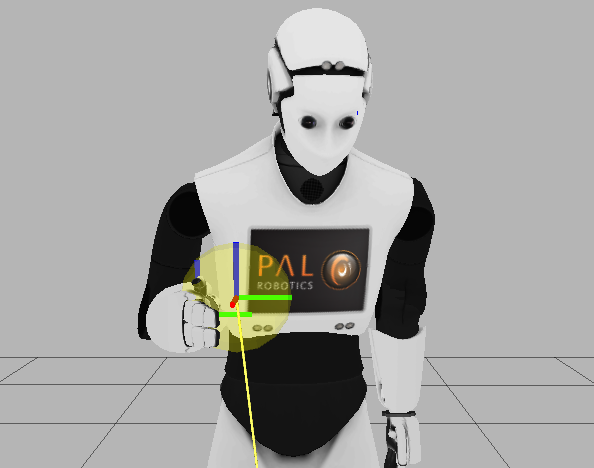
\includegraphics[width=0.23\textwidth]{../figures/object_moves/3.png}
  	}
  	  \subfigure[]{
  		\label{fig:objmoves4} 
  		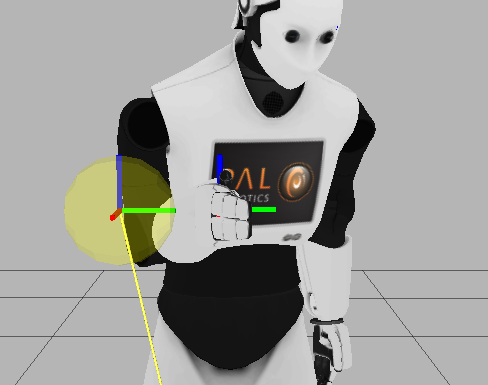
\includegraphics[width=0.23\textwidth]{../figures/object_moves/4.png}
  	}
  	  \subfigure[]{
  		\label{fig:objmoves5} 
  		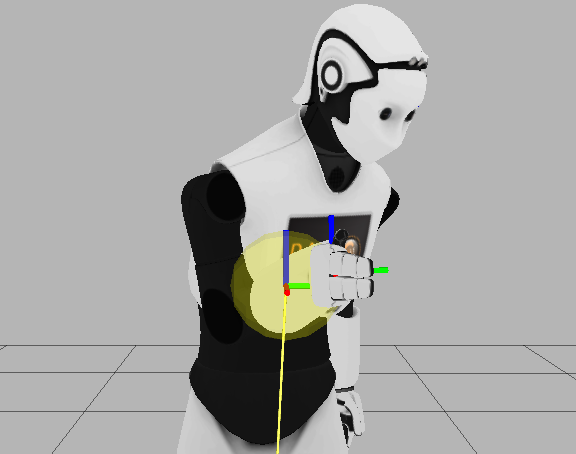
\includegraphics[width=0.23\textwidth]{../figures/object_moves/5.png}
  	}
  	  \subfigure[]{
  		\label{fig:objmoves6} 
  		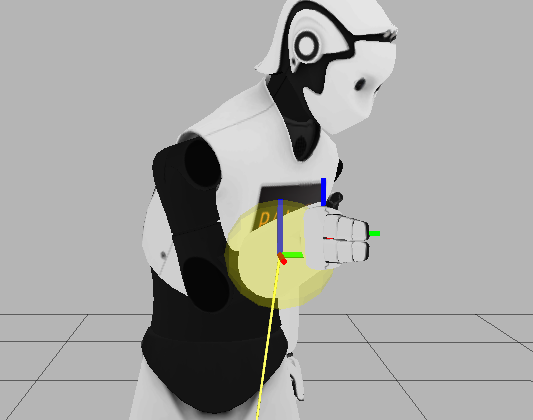
\includegraphics[width=0.23\textwidth]{../figures/object_moves/6.png}
  	}
  	  \subfigure[]{
  		\label{fig:objmoves7} 
  		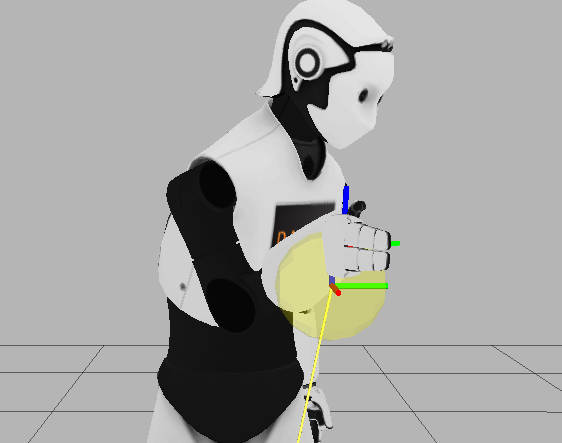
\includegraphics[width=0.23\textwidth]{../figures/object_moves/7.png}
  	}
  	  \subfigure[]{
  		\label{fig:objmoves8} 
  		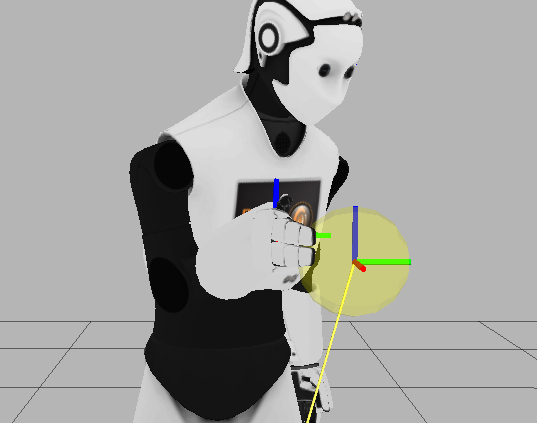
\includegraphics[width=0.23\textwidth]{../figures/object_moves/8.png}
  	}
\caption{Sequence of screen shots for the predefined trajectory. The yellow ball represents the moving external obstacle, which is not allowed to collide with the arm. Figure a)-d) the obstacle is approaching the fixed arm from the right. When the collision boundary is reached, the arm gets pushed away from the obstacle. In order to minimize the emerging position error, the arm moves along the negative $X$ and $Z$ axis to avoid the obstacle. This is shown in c). Figure e)-h): The obstacle moves closes from the left side. The solution for avoiding the obstacle is a displacement along a positive $Z$ axis.} 
    \label{fig:externobjectmoves}
\end{figure}

Equally, as in the previous experiment, the collision avoidance possesses a higher priority compared to the positioning task of the right wrist, which has the lowest priority. Due to this alignment of the stack, the right wrist leaves its desired position, when the collision avoidance becomes active in figure \ref{fig:objmoves2}. The obstacle pushes the arm away from its desired position in \ref{fig:objmoves3}. However, the positioning task is still active, which minimizes the emerged error. The resulting minimization of the error leads into a displacement along the negative $X$ and $Z$ axis. Finally, the arm avoids the moving obstacle and resolves to its original desired position (figure \ref{fig:objmoves4}). 
\newpage
The second row (figure \ref{fig:objmoves5} - \ref{fig:objmoves8}) describes the counter movement, where the obstacles approaches the arm from the left side. To avoid the obstacle and to minimize the emerging error, the arm moves along a positive $Z$ axis. We can see the exact behavior of this description in diagram \ref{fig:objmovesposition}. 
\begin{figure}
  \centering
    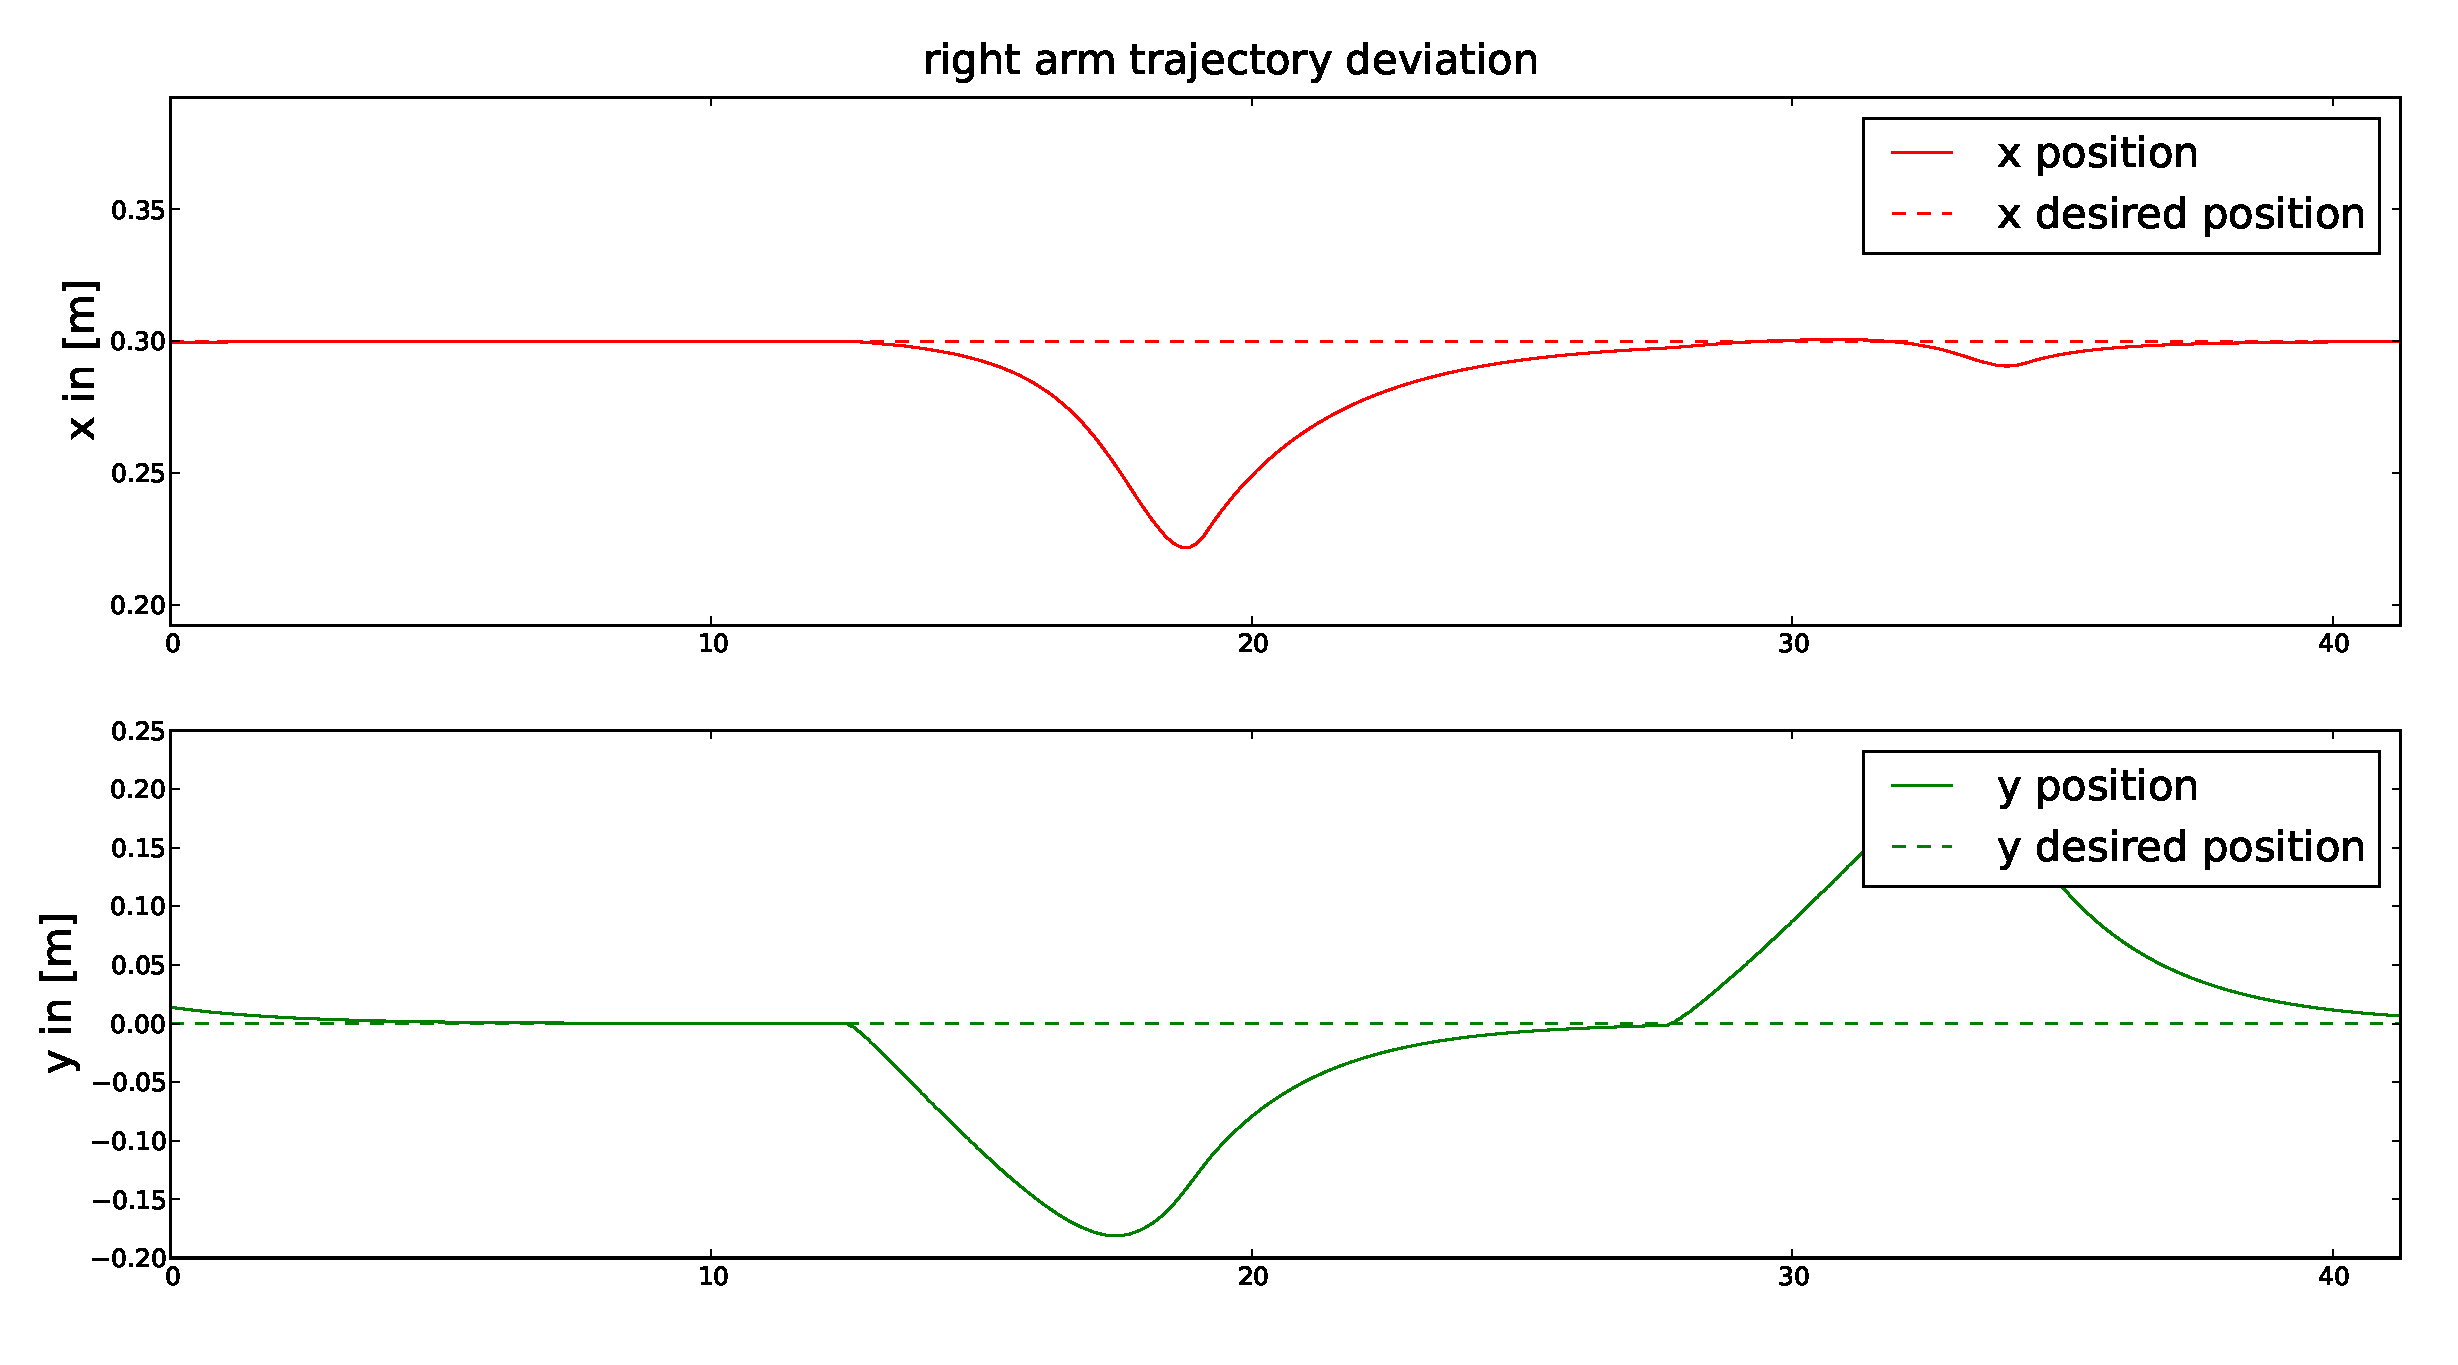
\includegraphics[width=\textwidth]{../figures/object_moves/position1.eps}
    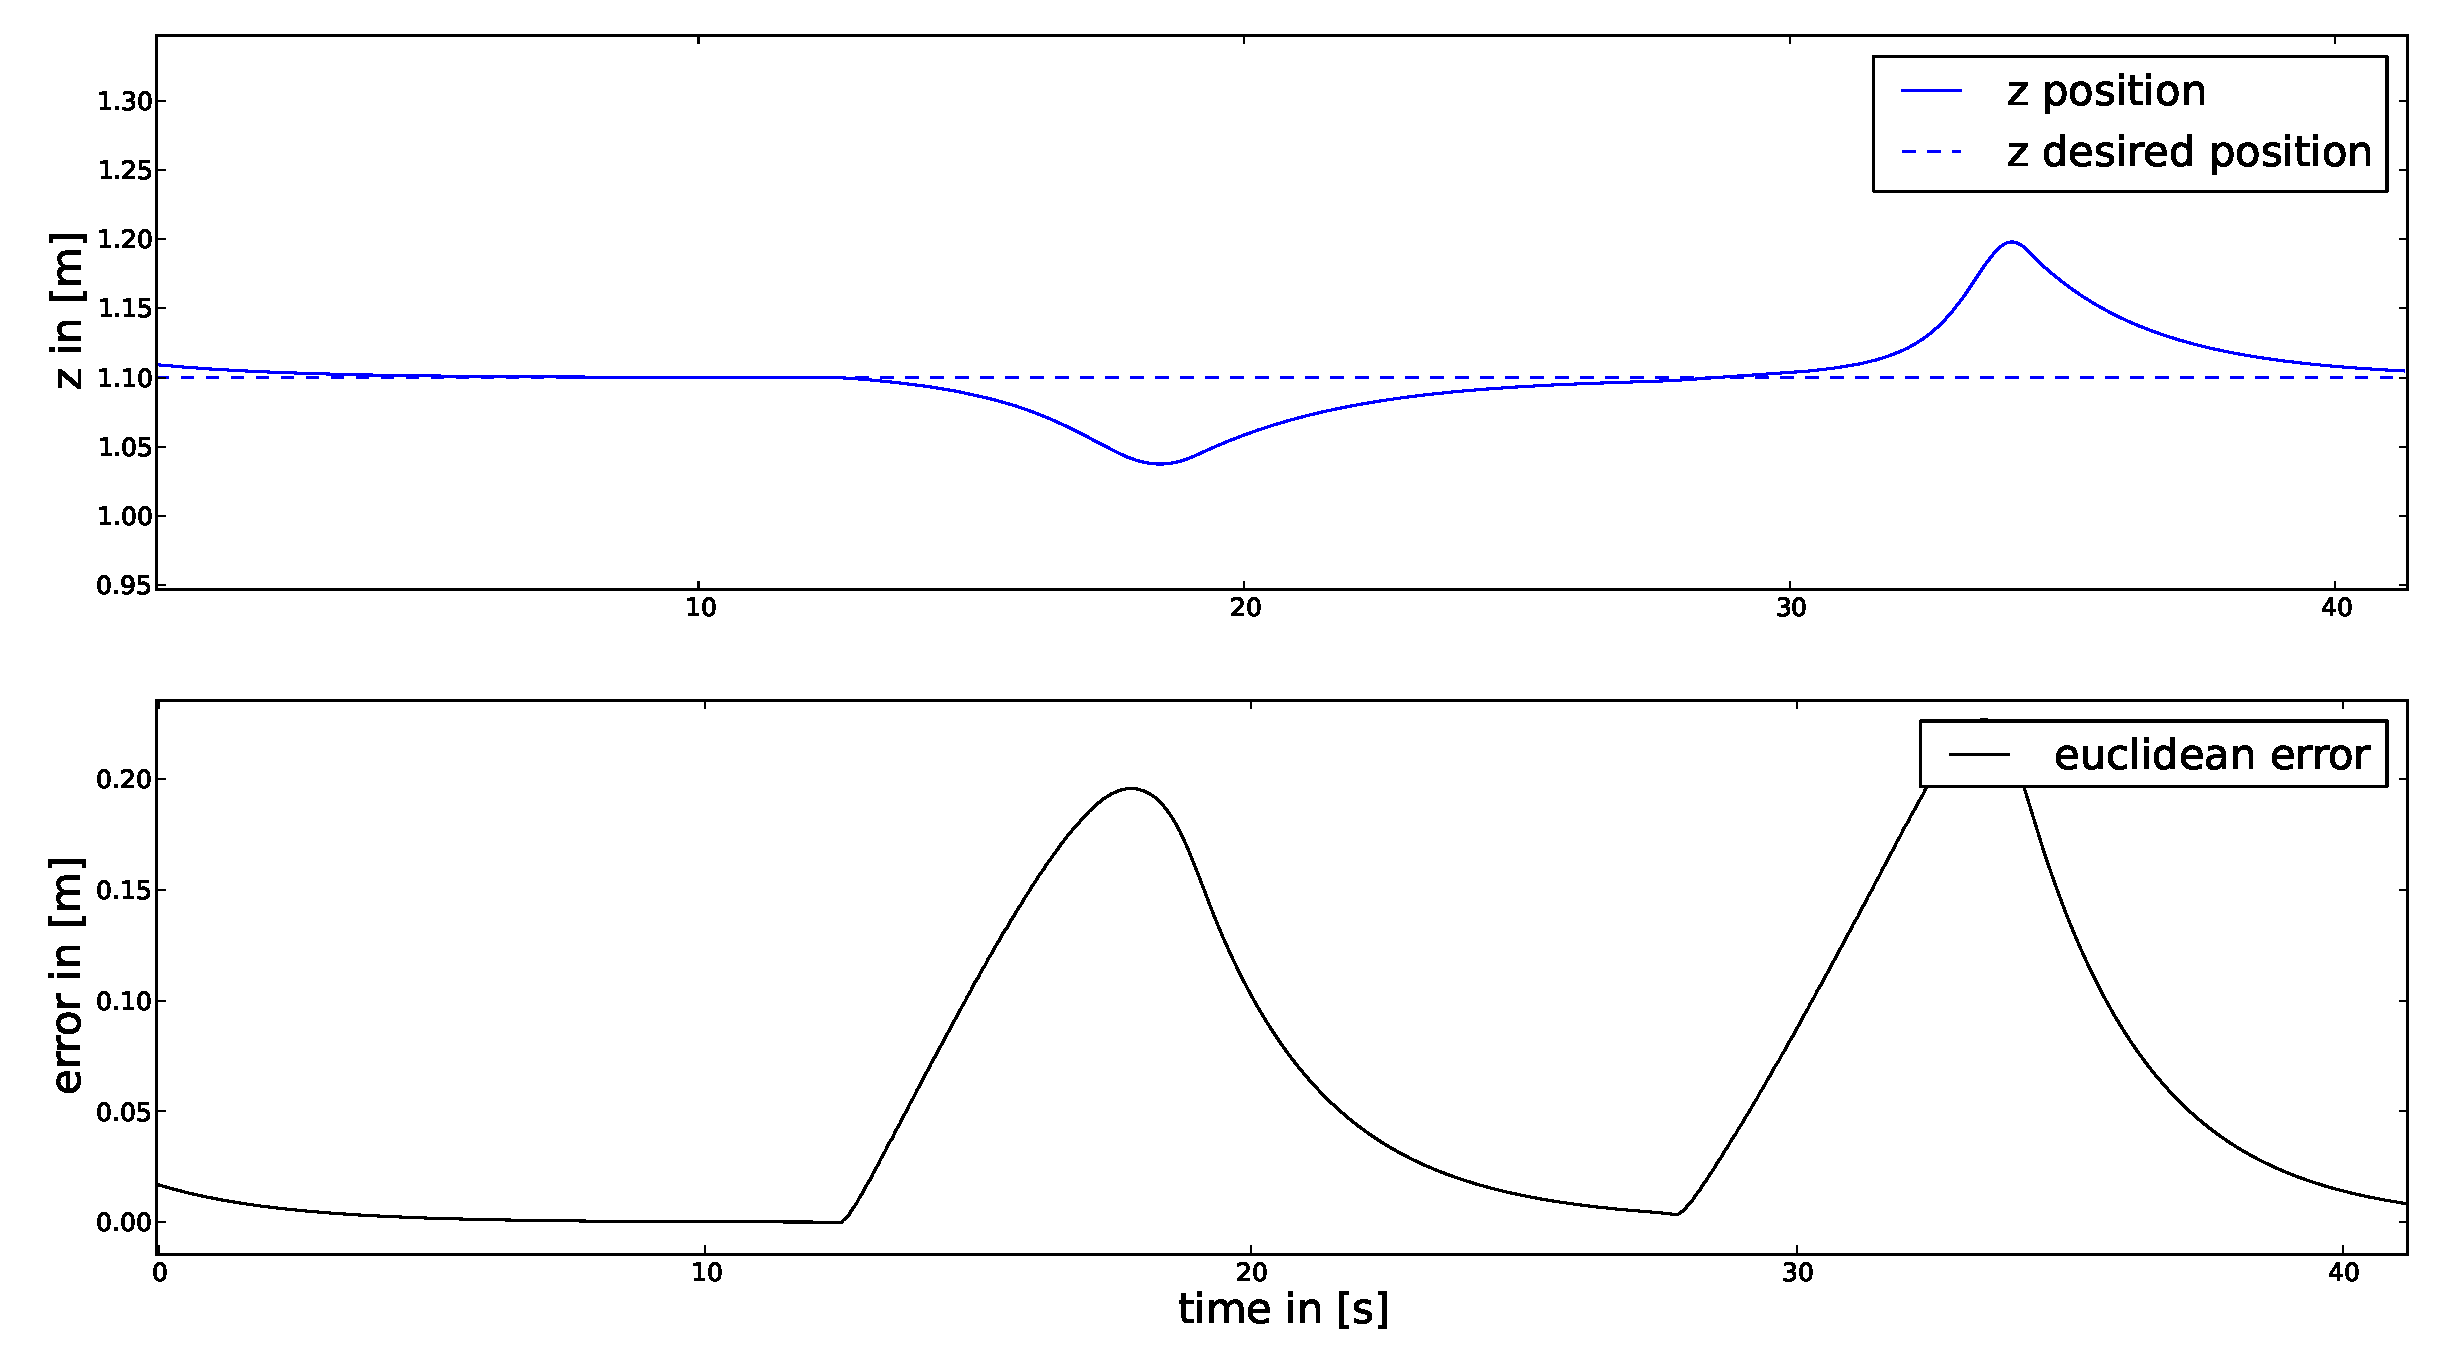
\includegraphics[width=\textwidth]{../figures/object_moves/position2.eps}
    \caption{Position plot over time. The obstacle gets avoided firstly by a negative movement in $X$ as well as $Z$. On the second approach, the avoidance happens by a movement in $Z$.}
    \label{fig:objmovesposition}
\end{figure}

The distance boundary $d_s$ was again set to $0.1m$. When we have a closer look at the distance development, we expect a similar behavior as in the previous test. The minimum boundary of $0.1$ is not allowed to get violated. 
Figure \ref{fig:objmovesdistance} provides information about the numerical exact distance. 
\begin{figure}
  \centering
    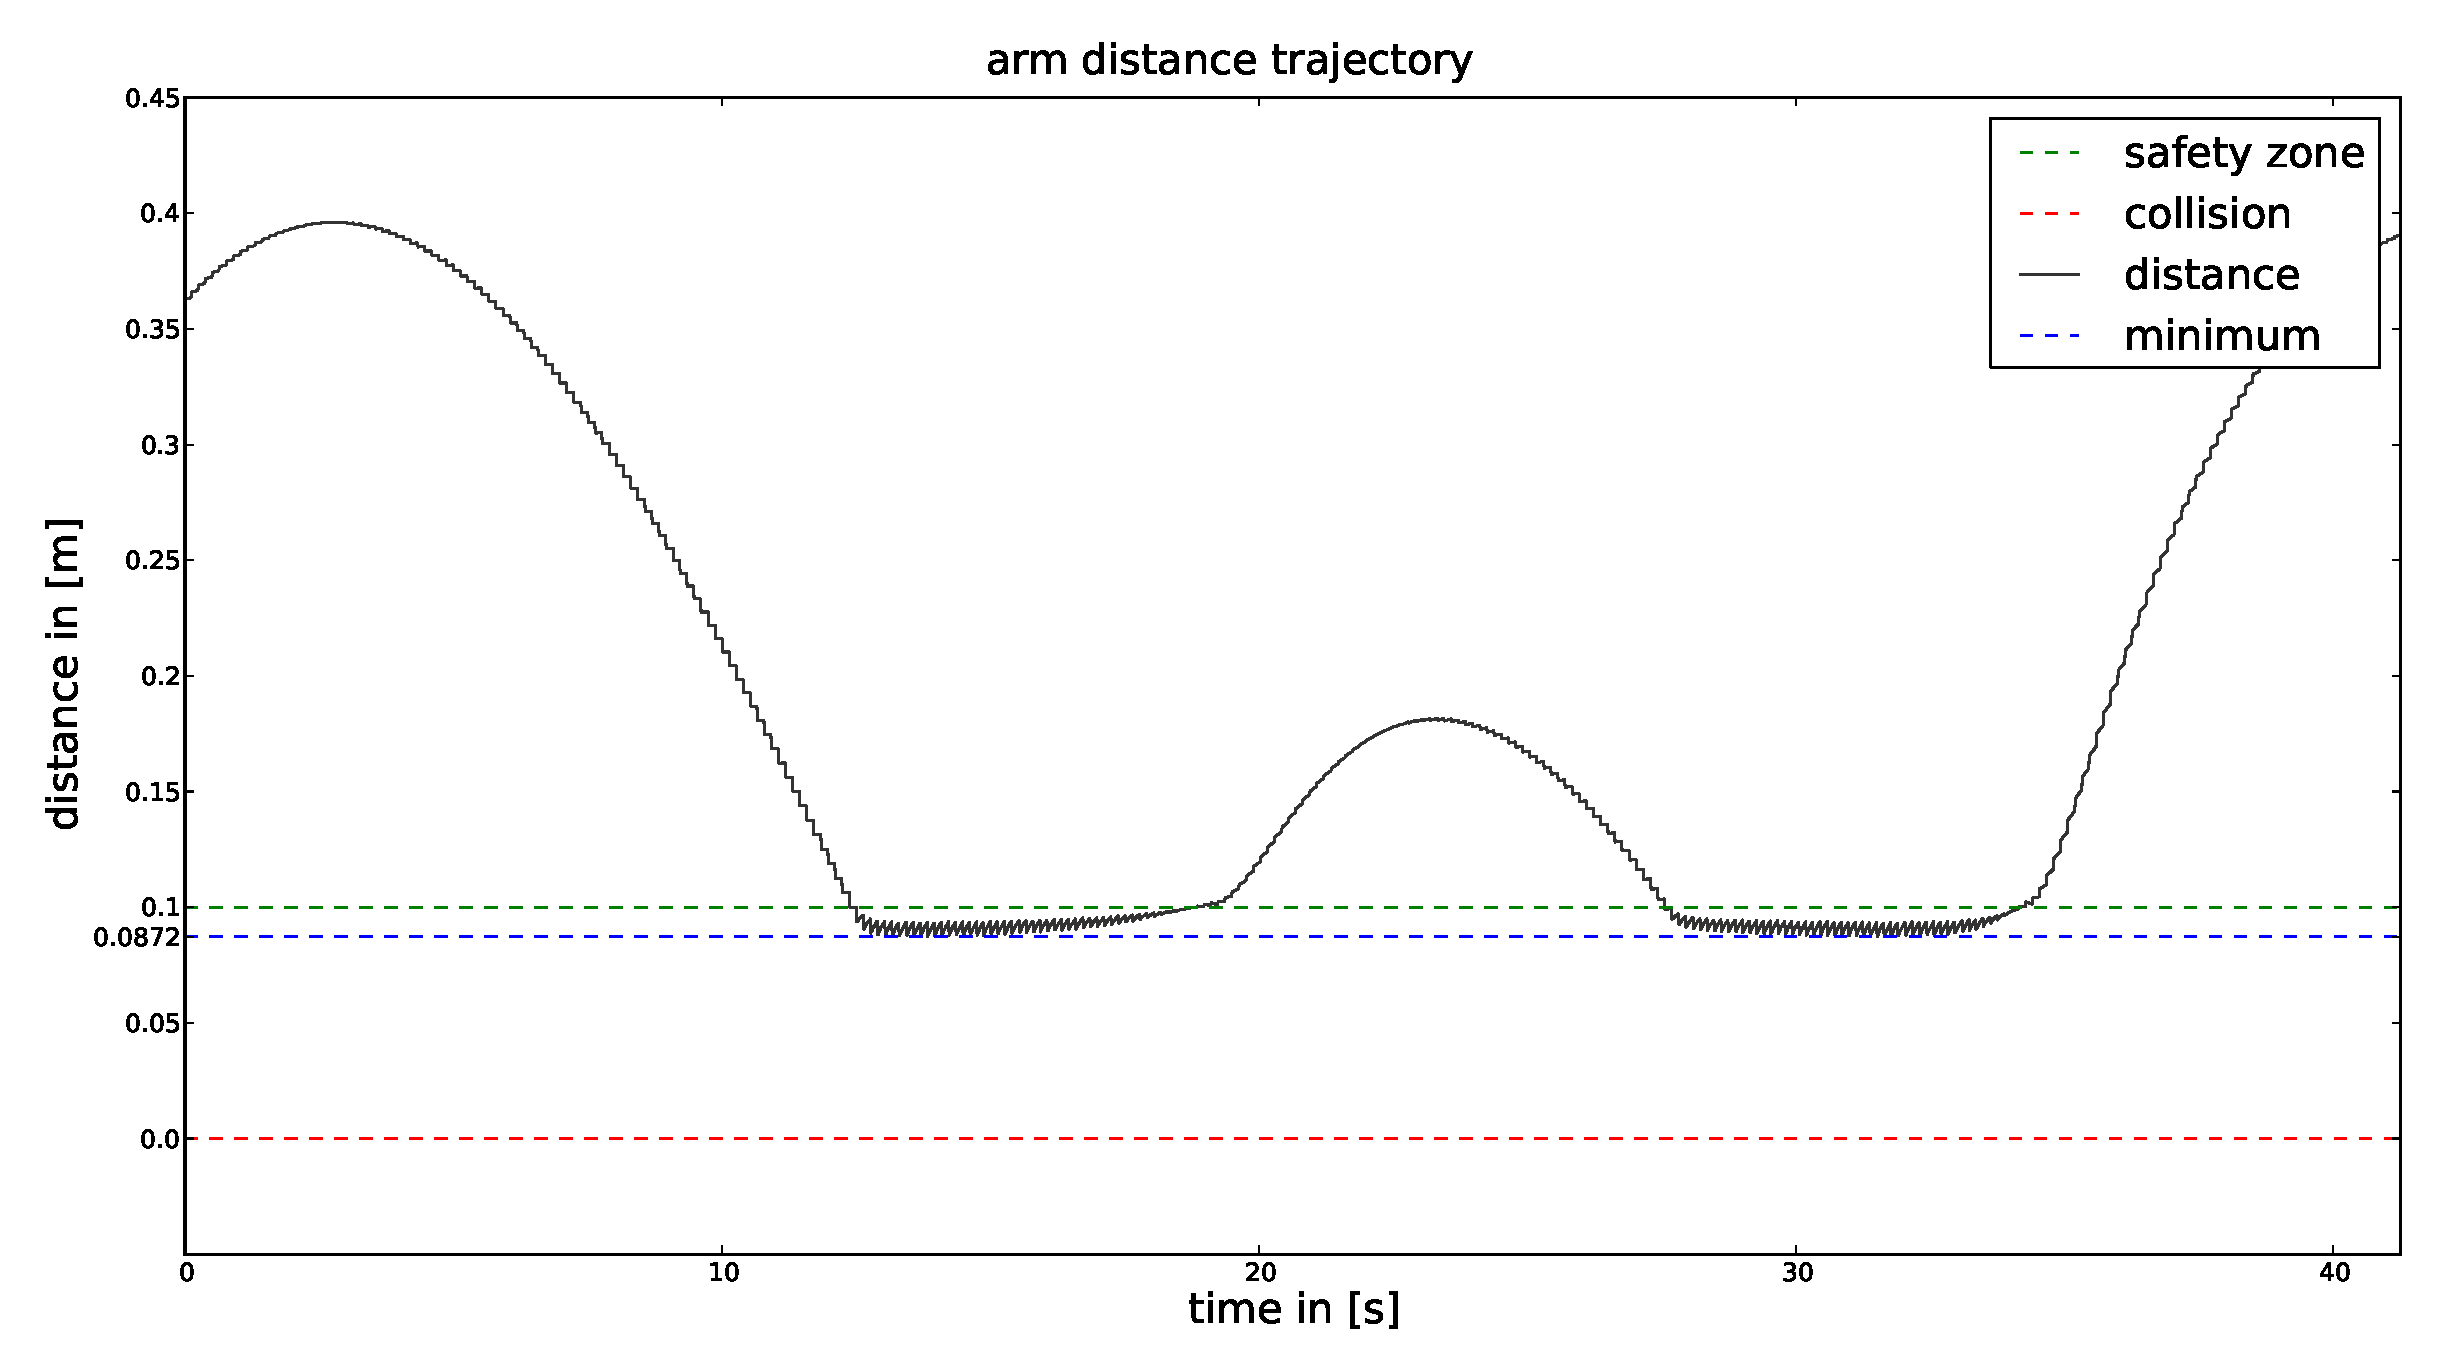
\includegraphics[width=\textwidth]{../figures/object_moves/distance.eps}
    \caption{Distance plot over time. The control gain are set to $\epsilon=10$, as well as $k=10$ for the positioning task. We can clearly see, that the safety distance is violated.}
    \label{fig:objmovesdistance}
\end{figure}

Contrary to our expectations, we see that the minimal boundary is violated. The minimal distance is not $0.1m$ but $0.872m$, which is a violation of approximately $13\%$. Furthermore, we can see a rather high frequent oscillation, once we hit the violation. 

In order to compensate for the violation as well as the oscillation, we retry the same experiments with a variation of the control gain $\epsilon$. 
Firstly, we set $\epsilon$ to a really high number such as $10000$ to see a tremendous chance, which can give possible insights about the reason for the violation. When we zoom in, we see the following result as depicted in figure \ref{fig:objmovesdistancek10000}.
\begin{figure}
  \centering
    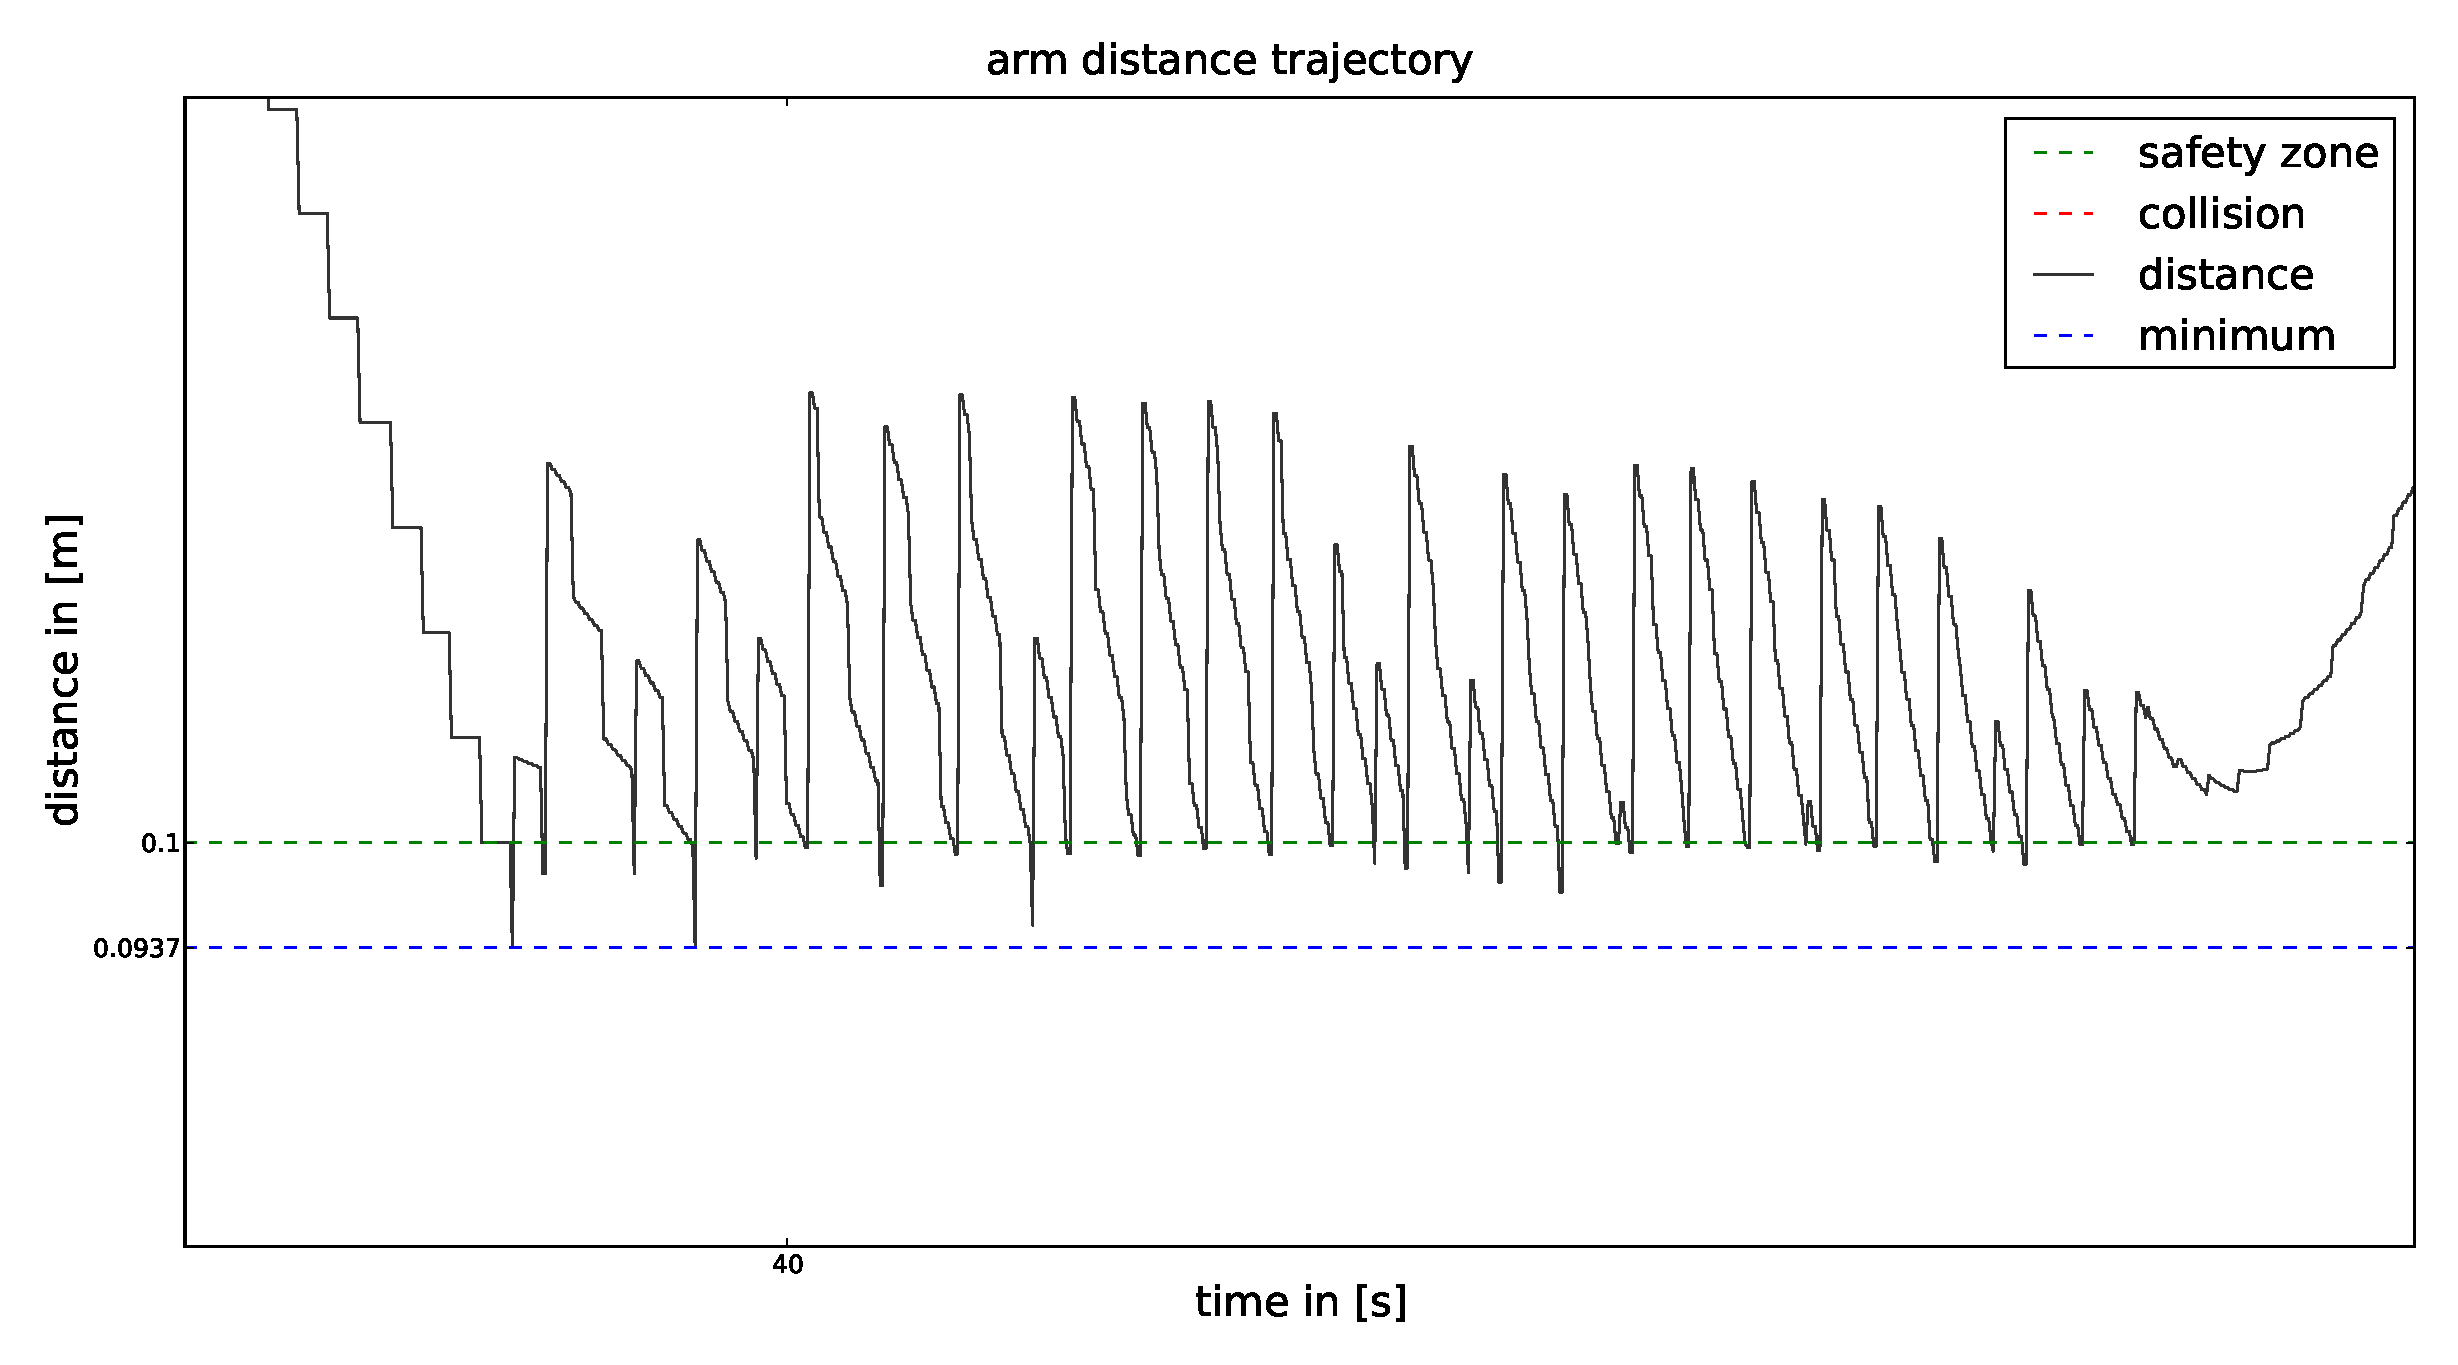
\includegraphics[width=\textwidth]{../figures/object_moves/distancek10000.eps}
    \caption{Behavior of a huge control gain for the velocity damping task. Here, $\epsilon$ is set to $10000$. We can see that the violation still occurs, but in a smaller quantity. However, the resulting oscillation increases dramatically, which results in heavy discontinuities in the velocity domain.}
    \label{fig:objmovesdistancek10000}
\end{figure}

The figure in \ref{fig:objmovesdistancek10000} evinces a lower distance violation of $7\%, (0.937m)$ compared to the $13\% (0.872m)$ before. However, a violation still occurs with a heavily amplified oscillation, which contains huge discontinuities. These discontinuities in distance yield to a huge velocity, hence to a clearly noticeable shaking of the robot arm.

The second try to optimize this undesired behavior is to lower the gain. Thus, we redo the experiment with an $\epsilon$ of $0.01$. Again, the distance development over time is plotted below (see figure \ref{fig:objmovesdistancek1}).
\begin{figure}[h!]
  \centering
    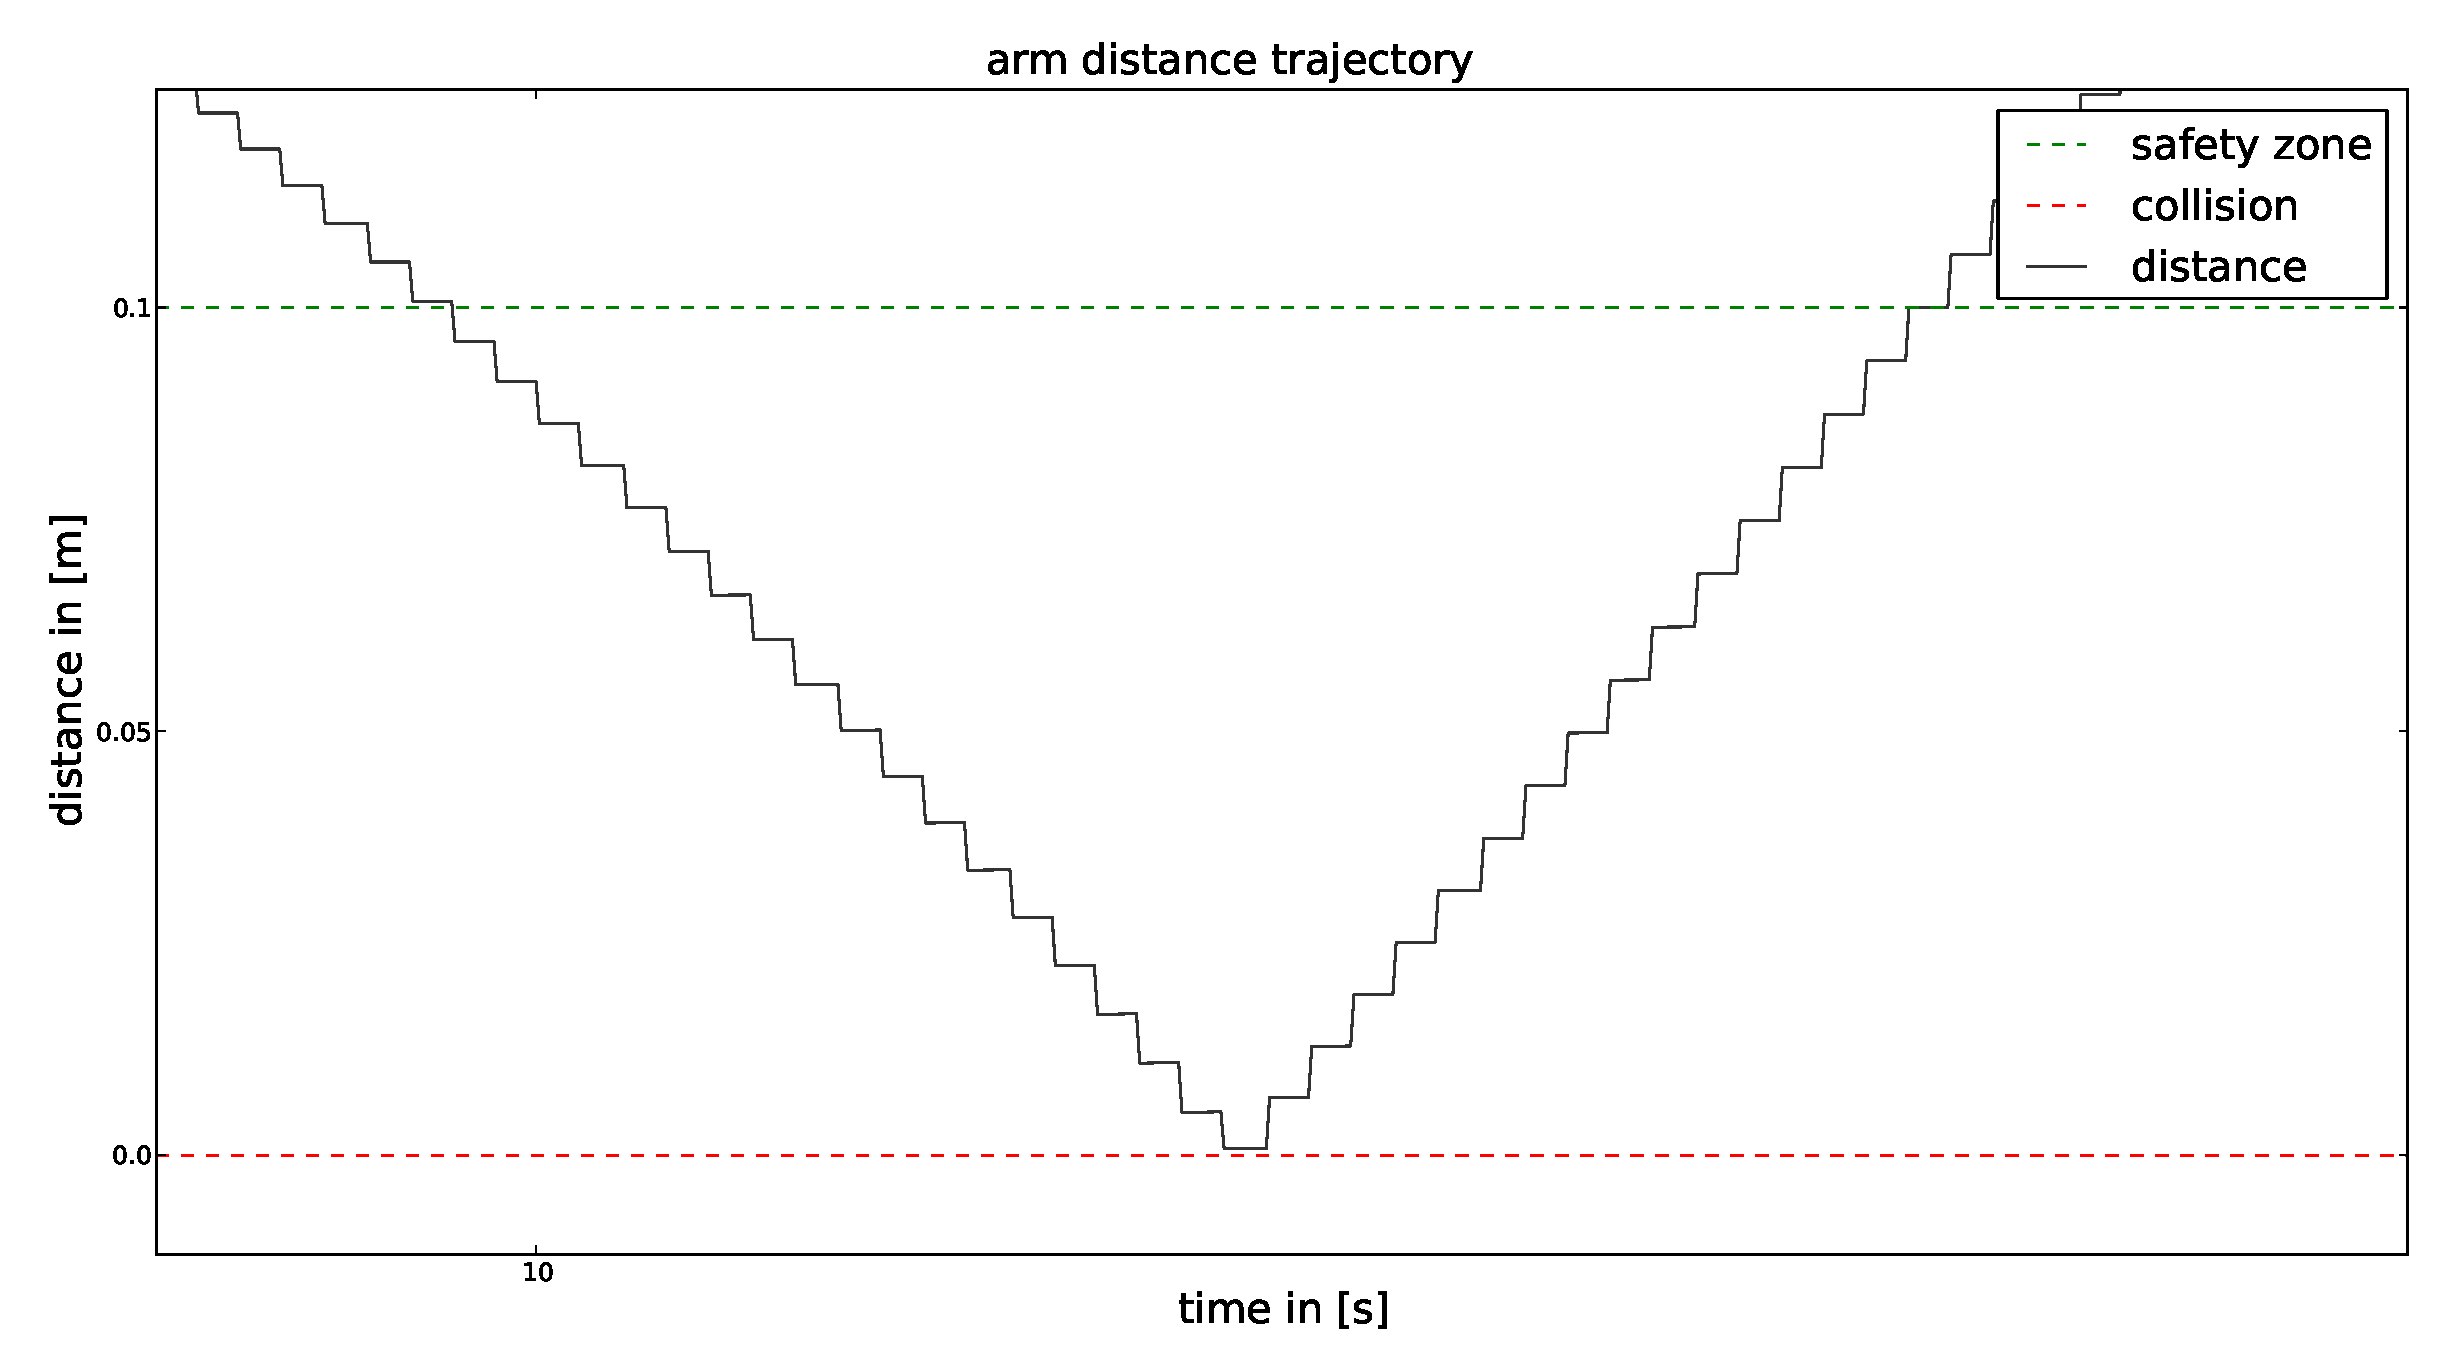
\includegraphics[width=\textwidth]{../figures/object_moves/distancek001.eps}
    \caption{Behavior of a low control gain for the velocity damping task. Here, $\epsilon$ is set to $0.01$. We encounter a full collision and absolutely no attempt to avoid the obstacle. However, no discontinuities occur.}
    \label{fig:objmovesdistancek1}
\end{figure}

Figure \ref{fig:objmovesdistancek1} reveals the bottleneck of this method for avoiding obstacles. The control gain $\epsilon$ is set to $0.01$, which yields in no obstacle avoiding, since the minimal distance shrinks to $0.0m$, which is a full collision. Moreover, we can see that the right arm has a slow velocity, which yields, contrary to a control gain of $\epsilon=10000$,  into no heavy shaking of the robot. However, the velocity is way too small to avoid the obstacle in time.

Thus looking at the two variations, it becomes clearly that for this use case of accelerating a body part with zero initial velocity, special care has to be taken in gain tuning. When we want to provide service for any external velocities, the control gains have to be tuned according to the estimated velocity of the external obstacle. As we could see within this outcome, we have to find a trade-off between highly reactive body parts and lowest distance boundary violations. 

The important issue however, is that in all variations in $\epsilon$ the boundary gets violated. We discuss the nature of this in the next section \ref{sec:results}, where we analyze the reason this for in more detail.

\subsection{Self-Collision Avoidance}
As an enhancement of the collision avoidance task for external object, we examine now an avoidance of the robots body part itself. For the following concrete tests, we refer again to the capsule decomposition provided in table \ref{tab:capsules}. We consecutively test each group against each other. 
\begin{figure}[h!]
  \centering
    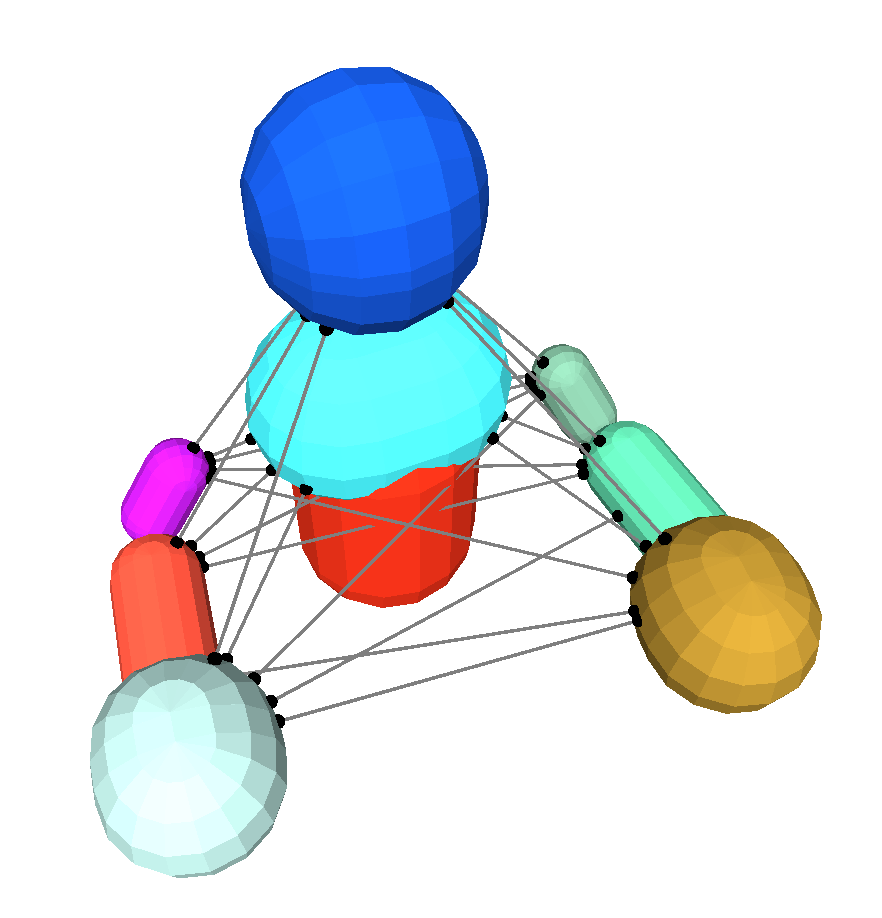
\includegraphics[width=0.48\textwidth]{../figures/closest_points_front.png}
    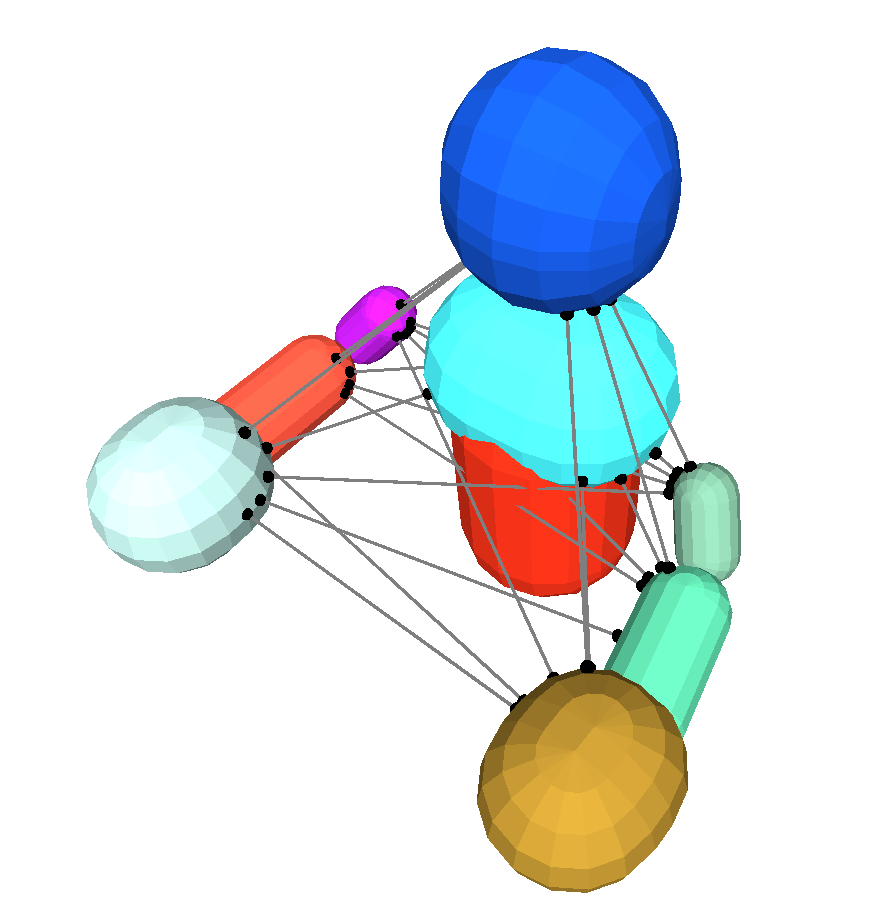
\includegraphics[width=0.48\textwidth]{../figures/closest_points_side.png}
    \caption{Visualization of the full collision matrix. Every collision pair is illustrated with its respective closest point pair onto the capsules surface. In this section, we examine all possible collision pairs with each other.}
    \label{fig:capsuleclosestpoint}
\end{figure}

We configure the velocity damping task according to each closest point pair, we take into consideration. Looking at figure \ref{fig:capsuleclosestpoint}, we illustrate the full collision matrix of possible colliding body parts with their respective closest points. In the remainder, we will test every point pair of this collision matrix. With this in mind, we test this collision matrix in a asynchronous, one-directional way. In particular, this means that, to begin with, we test the arms against the upper body as well as the head. As in the external collision avoidance, the arm tries to avoid the obstacle to its best. One-directional here denotes, that the arm avoids the upper body. However, the upper body does not avoid the arm. \\
Reasons for this decision were mainly to keep the number of constraints to a minimal configuration. Equally, the head and both torso links hold only one DOF, which brings just a little effect on avoiding 6 DOF of the arm. Furthermore, actively constraining the torso might have an bequeathing effect on the underlying wrist positioning task, since these links are commonly shared between both kinematic chains.
\begin{figure}[h!]
  \centering
  \subfigure[]{
  		\label{fig:armbody1} 
  		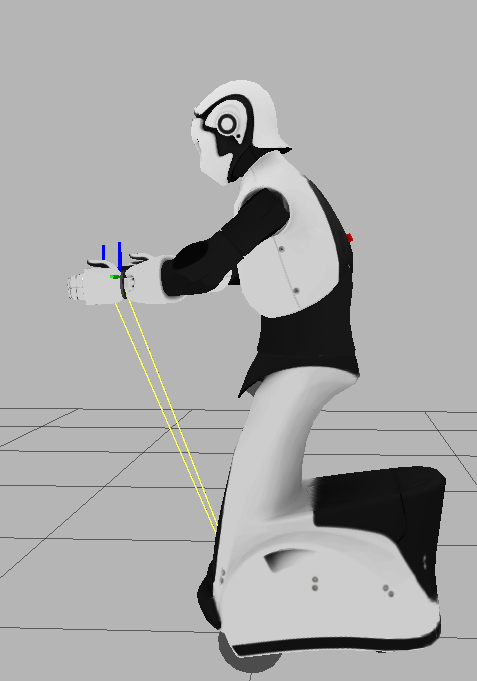
\includegraphics[width=0.148\textwidth]{../figures/arm_body/1.png}
  	}
  	  \subfigure[]{
  		\label{fig:armbody2} 
  		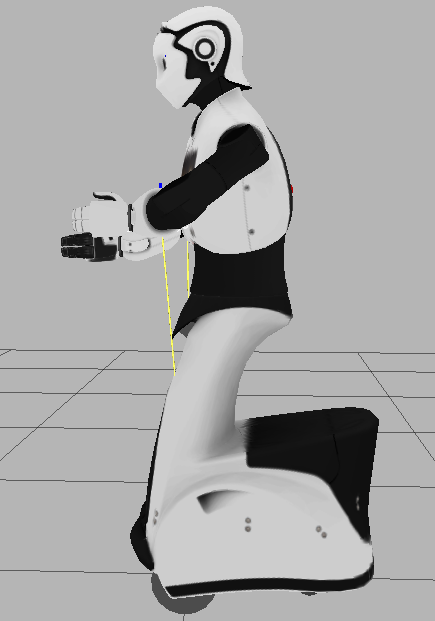
\includegraphics[width=0.148\textwidth]{../figures/arm_body/2.png}
  	}
  	  \subfigure[]{
  		\label{fig:armbody3} 
  		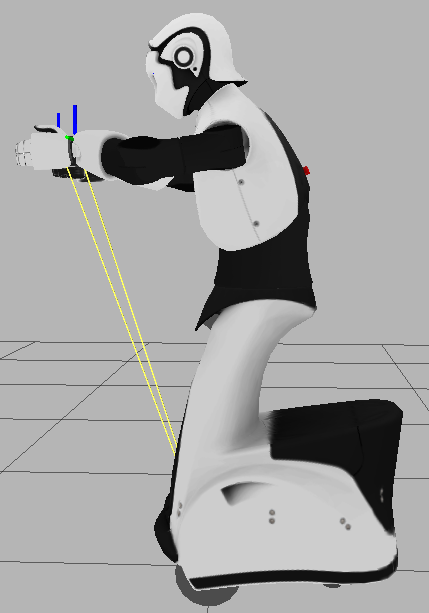
\includegraphics[width=0.148\textwidth]{../figures/arm_body/3.png}
  	}
  	  \subfigure[]{
  		\label{fig:armbody4} 
  		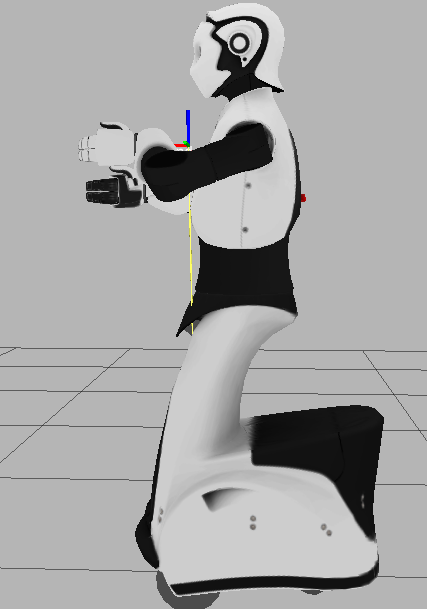
\includegraphics[width=0.148\textwidth]{../figures/arm_body/4.png}
  	}
  	  \subfigure[]{
  		\label{fig:armbody5} 
  		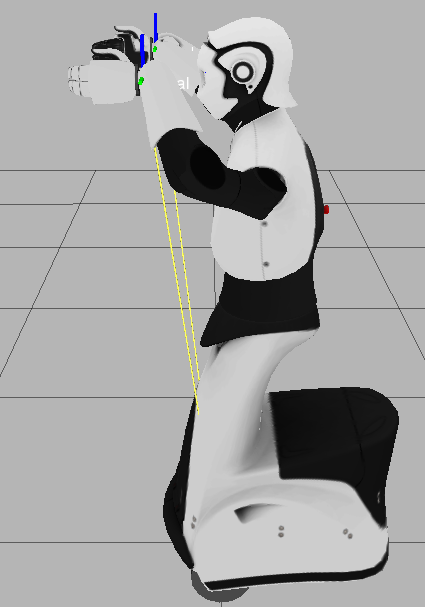
\includegraphics[width=0.148\textwidth]{../figures/arm_body/5.png}
  	}
  	  \subfigure[]{
  		\label{fig:armbody6} 
  		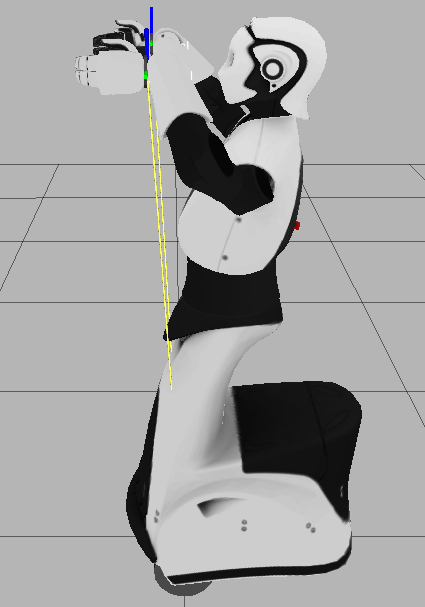
\includegraphics[width=0.148\textwidth]{../figures/arm_body/6.png}
  	}
  	\caption{Executed trajectory for the following self-collision experiment. We lead the arms into three possible collisions. Figure a)-b) would result in a collision with the lower torso, figure c)-d) equally with the upper torso. Finally, figure e)-f) illustrate a collision with the head. Thus, we describe a trajectory which alternates as a sine waves along $X,Y$ as well as a three step increase along $Z$.}
	\label{fig:armbody}
\end{figure}
\newpage
In the remainder of this section, a similar trajectory as the one depicted in figure \ref{fig:armbody} is executed. We can see, that we firstly set a goal position at the internal of the lower torso (figure a)-b)). We increase the height and repeat the same movement to provoke a collision with the upper torso (figure c)-d)). Finally, we repeat it equally with the head position (figure e)-f)). 

We can see the resulting positioning diagram in figure \ref{fig:selfcollisionposition}. At approx. $t=25s$, we shift the collision center from the lower torso to the upper torso. Similarly, we aim for colliding with the head at $t=70s$. We do not specify this position plot in more detail in any further experiment. We do this for simplicity reasons as the specified trajectory is mirrored for the left and right arm, which in the end results in a similar plot regardless the configuration of the positioning tasks.
\begin{figure}[h!]
  \centering 
     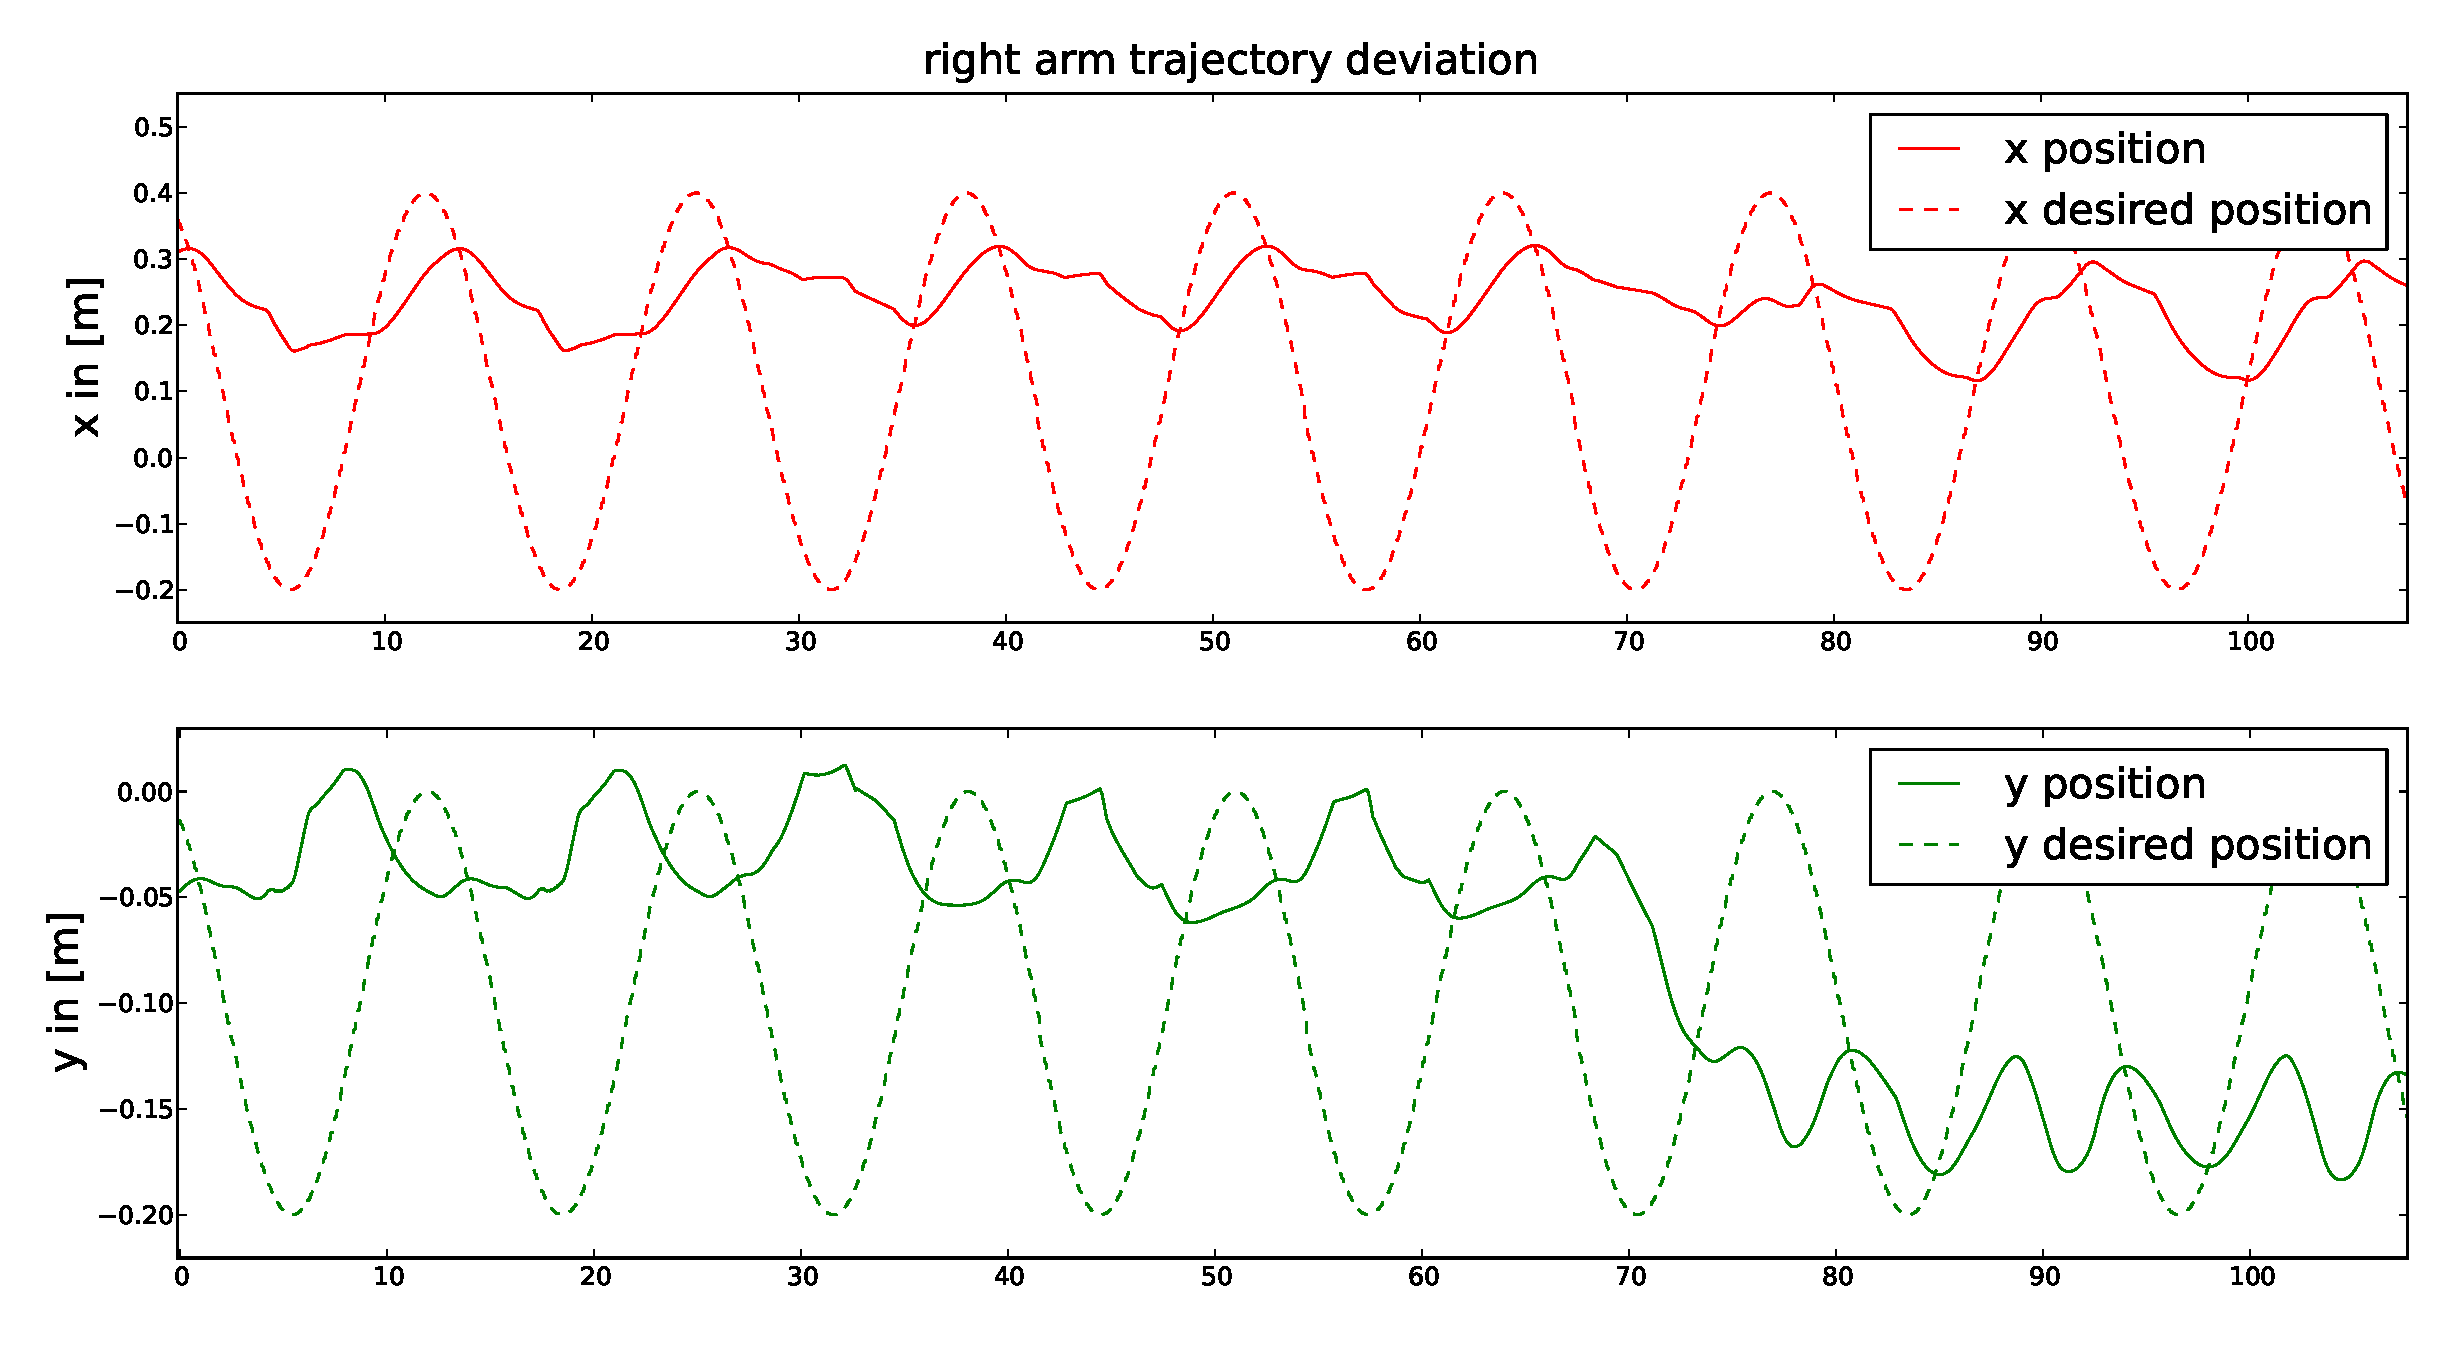
\includegraphics[width=\textwidth]{../figures/arm_body/position1.eps}
     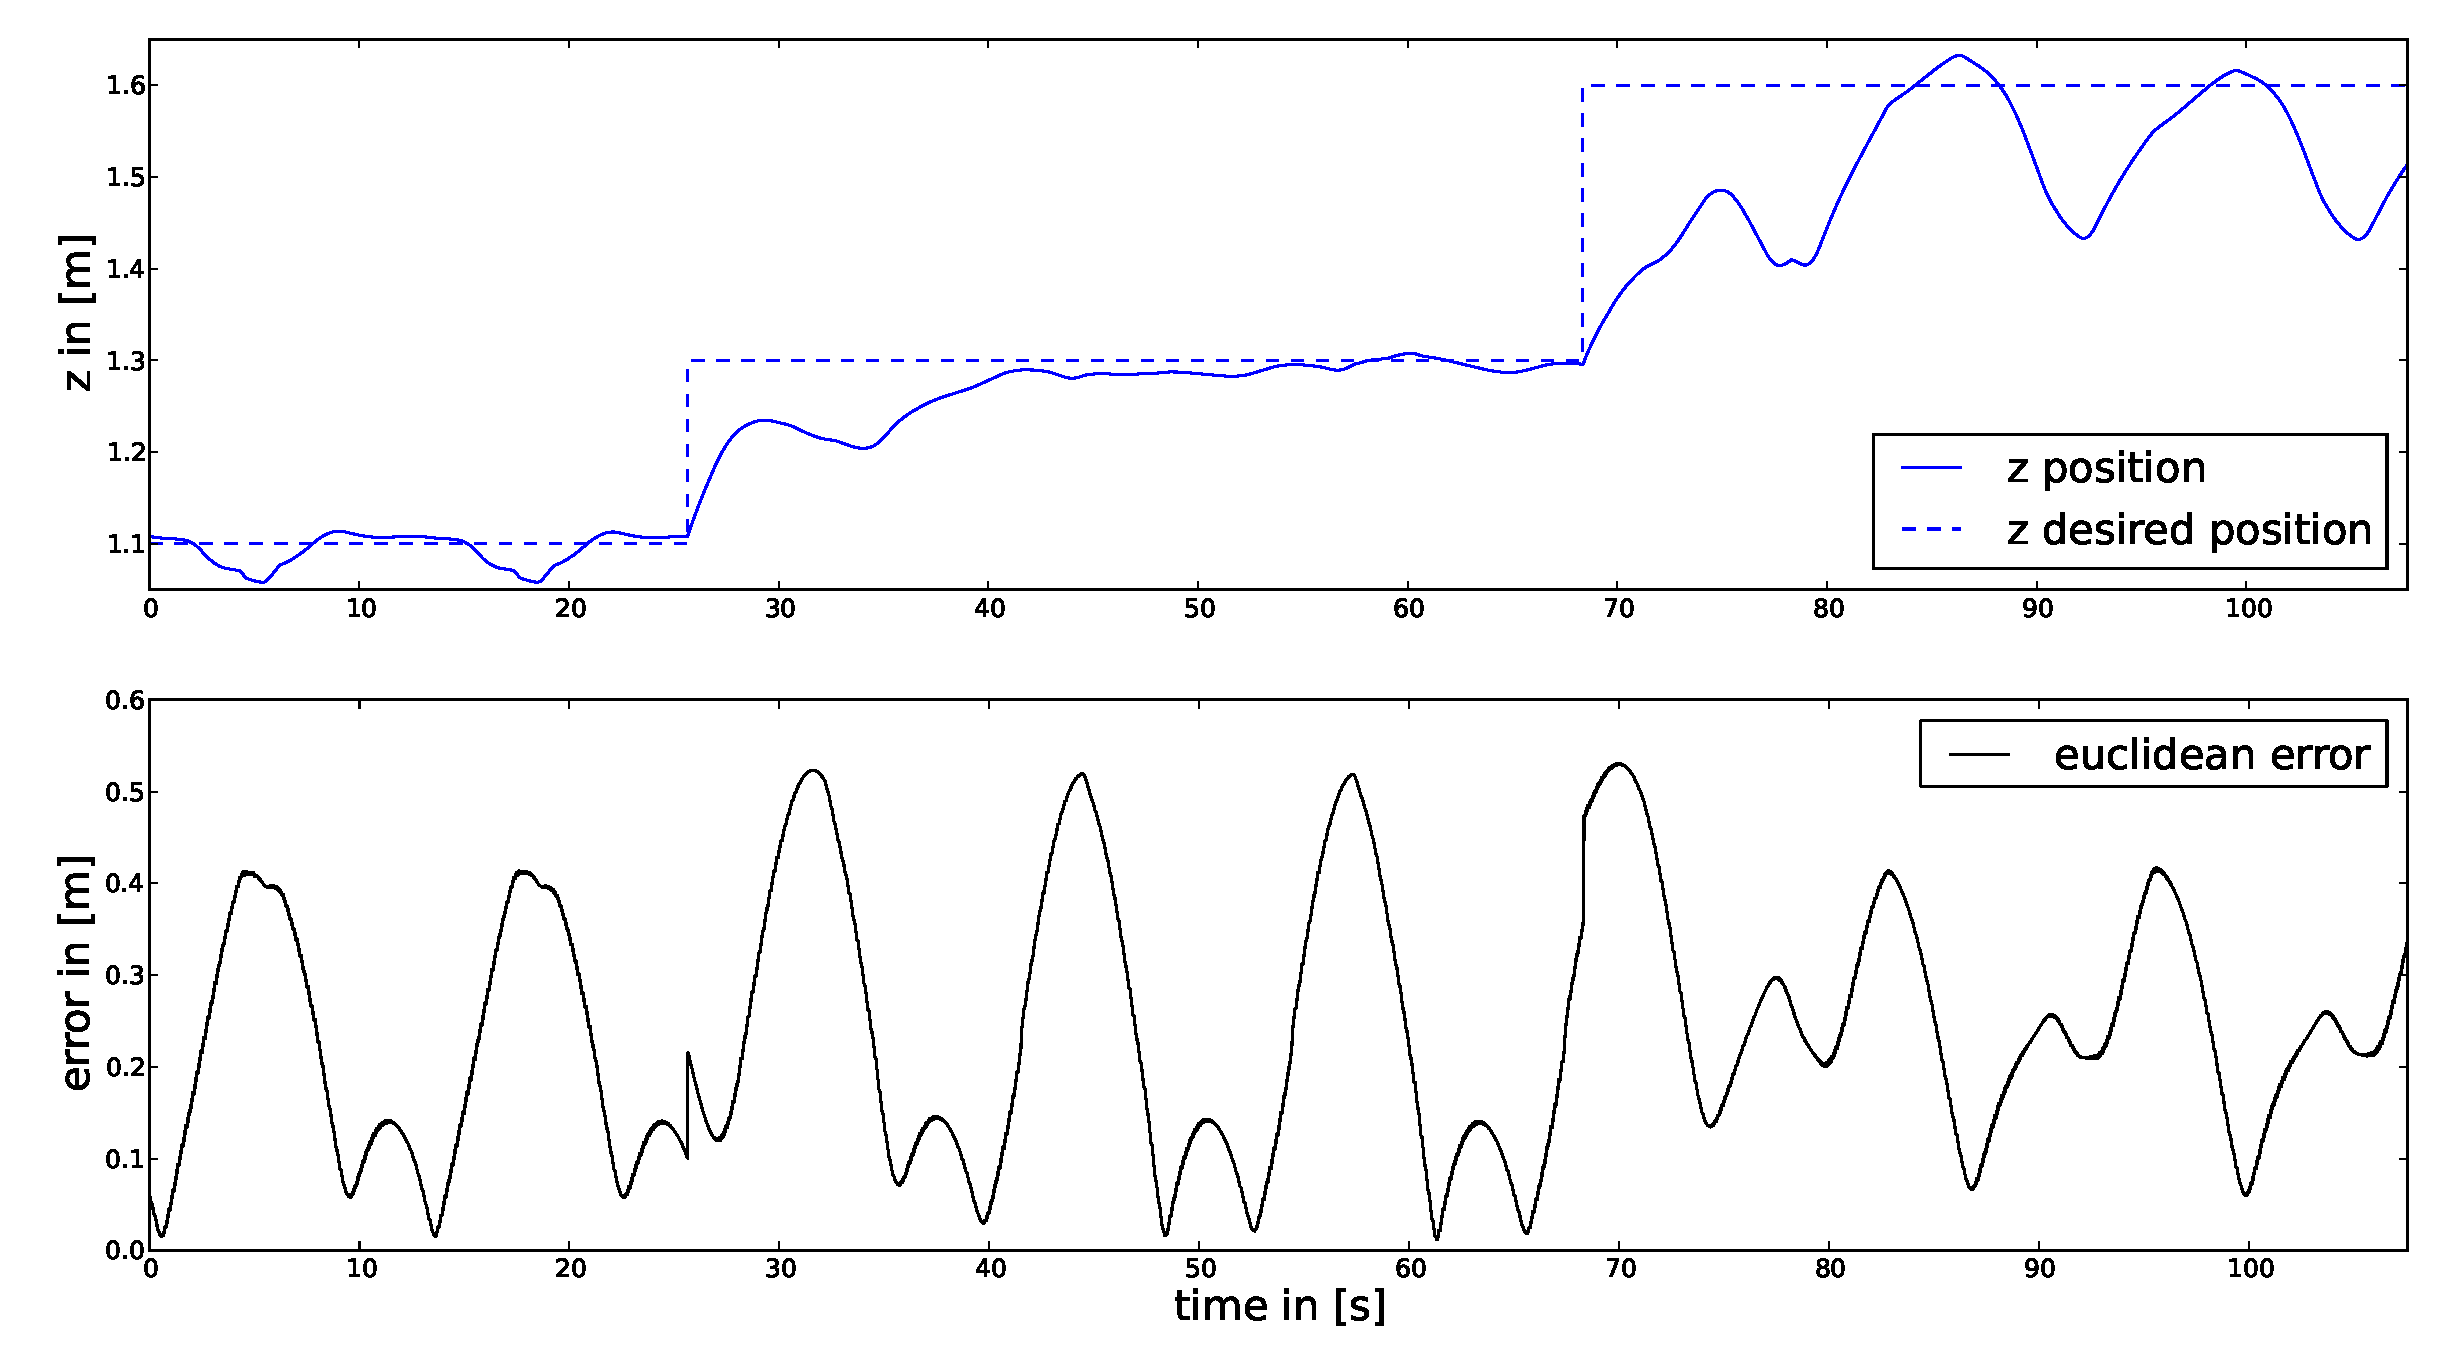
\includegraphics[width=\textwidth]{../figures/arm_body/position2.eps}
    \caption{Positioning diagram of the applied trajectory for self-collision test. As we can see in the development of along the $Z$ axis, we increase the height in three steps: Lower torso, upper torso and head. We can assume an almost similar plot, independent whether a single arm or both are on the stack.}
    \label{fig:selfcollisionposition}
\end{figure}

\clearpage
\subsubsection*{Arms vs. Upper Body \& Head}
To begin with, we test the collision between one arm and the torso, which is quite likely to occur during common movements. Depending on the desired goal position, the minimal cost trajectory often leads through the torso. Thus, we start our examination on self-collision avoidance by repeatedly specifying a goal position for the arm, which is inside the upper body and head, respectively. 

The control gain for the two tasks of main interest are set to $\epsilon=10$ for the velocity damping as well as $k=10$ for the positioning task.   
A cumulated distance plot is displayed in \ref{fig:selfcollisiondistance}. We see that the violation zone gets not violated except from numerical errors. We can take the violations as numerical errors since the violation does not depend on $\epsilon$. We reproduced the experiment with different variations of $\epsilon$ with equally important results. Furthermore, looking at the numerical value of these violations, we can see a violation of $0.003m$, which essentially denotes a violation of $3mm$.  
\begin{figure}[h!]
  \centering
    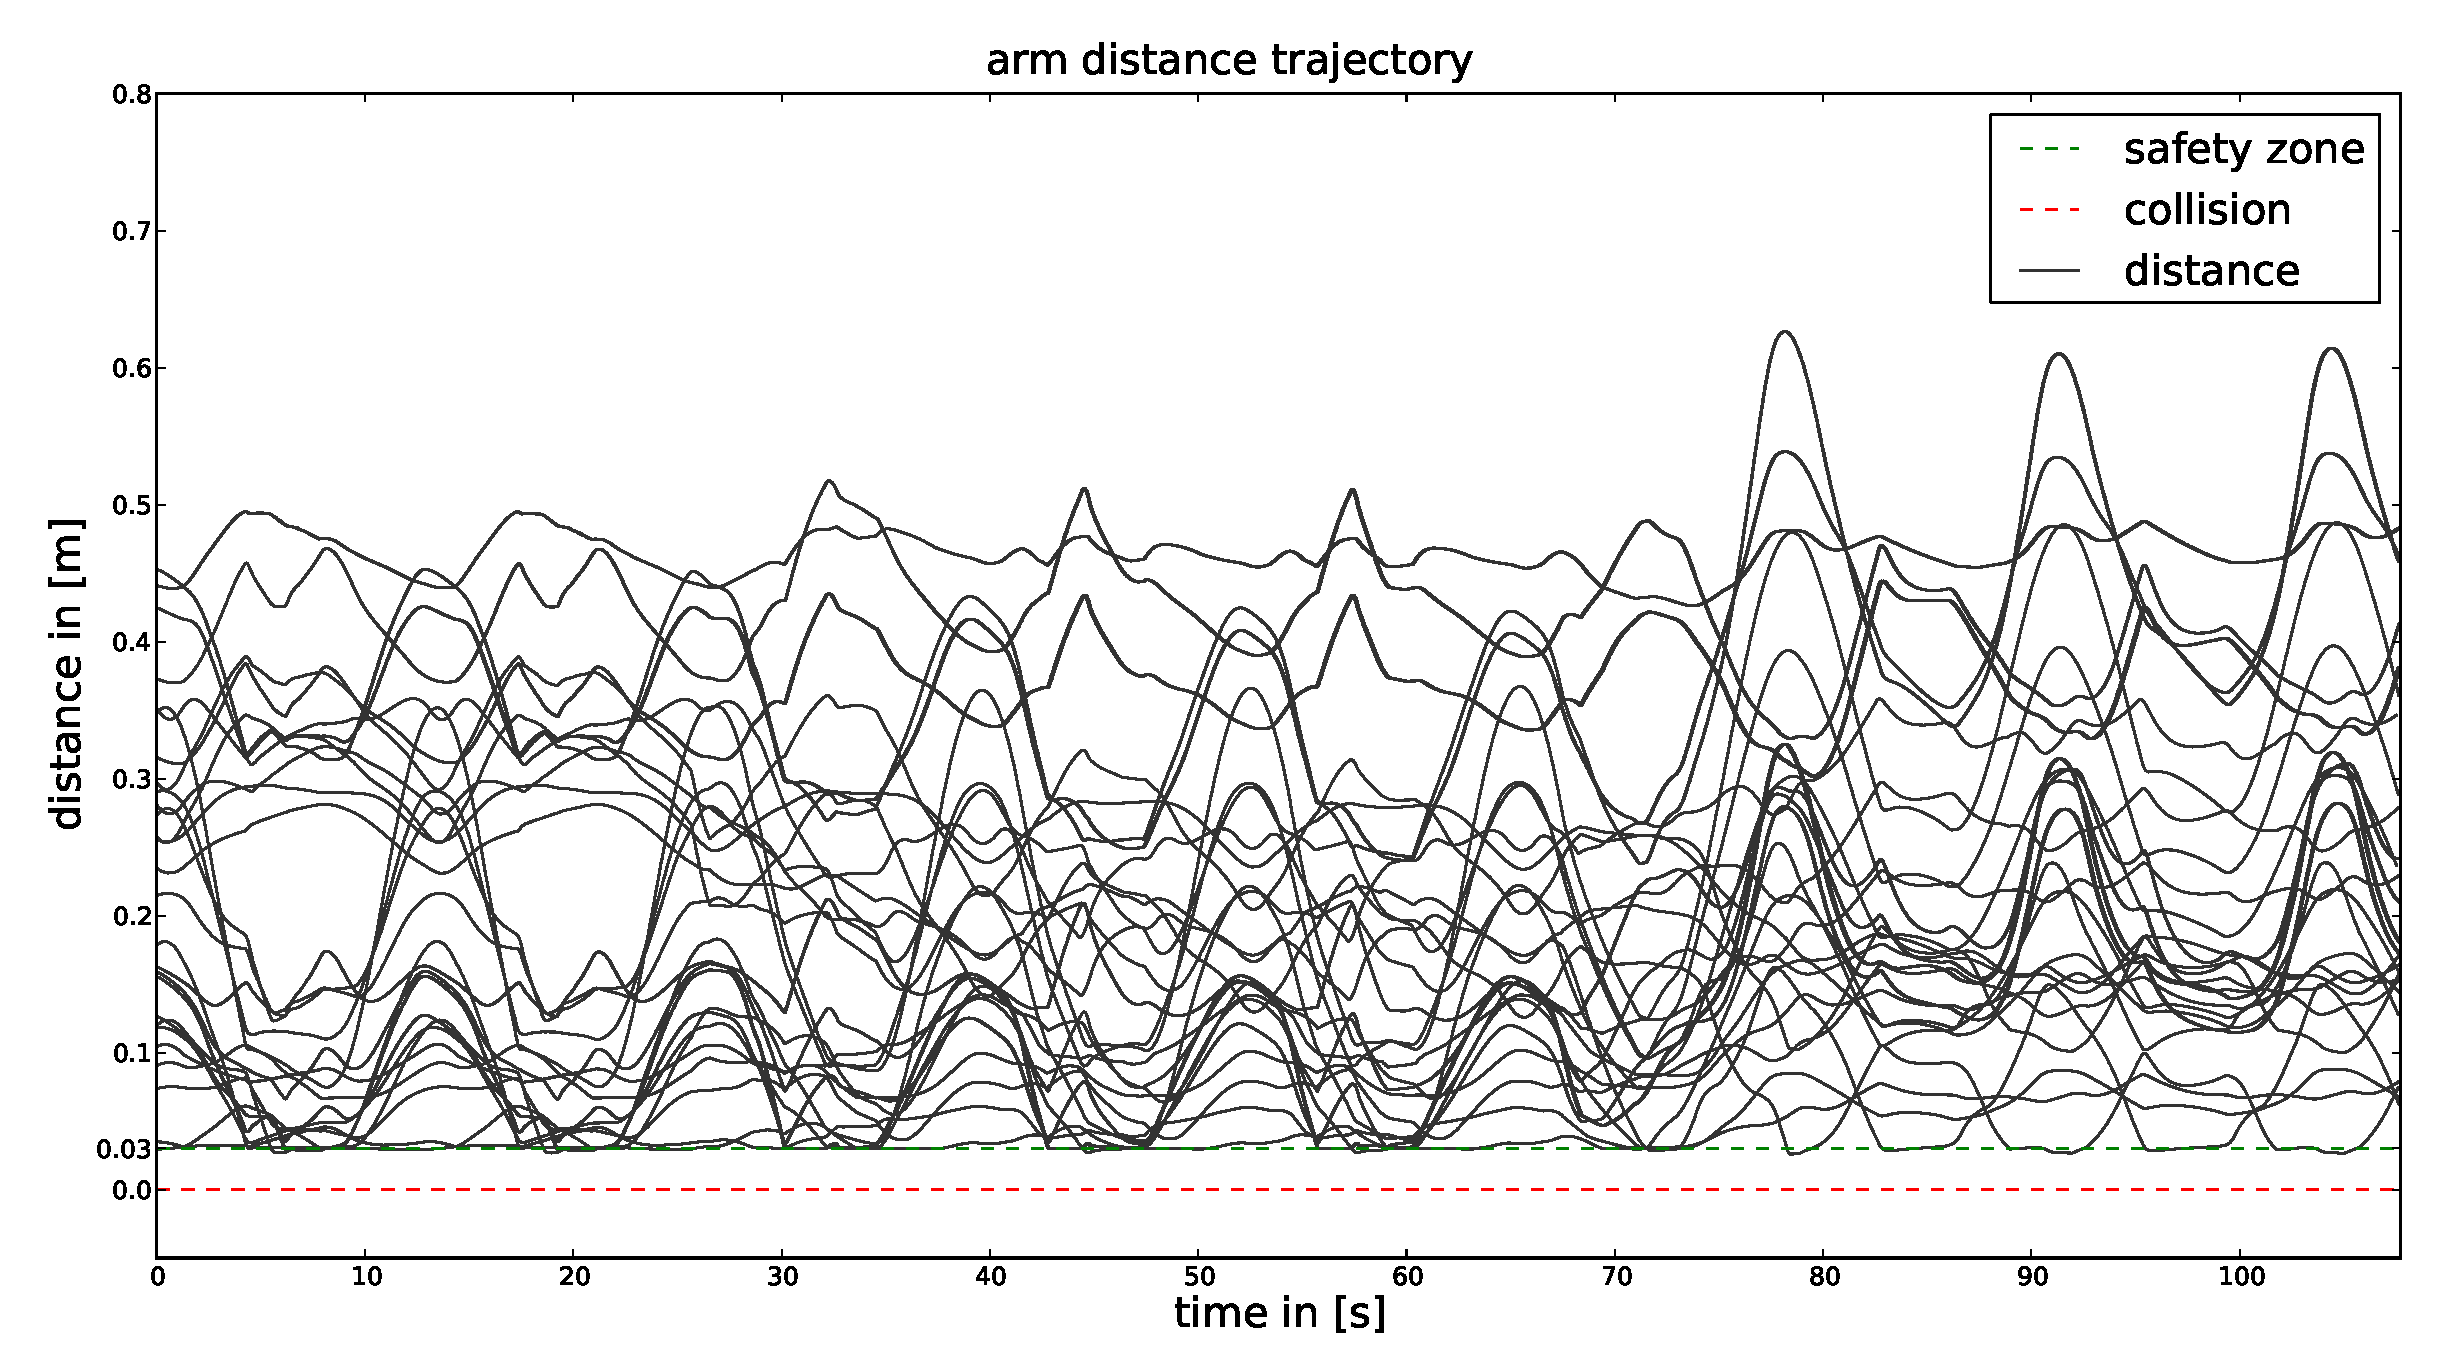
\includegraphics[width=\textwidth]{../figures/arm_body/distance.eps}
    \caption{Distance plot over all tested collisions. We can see that except numerical issues, we do not have a tremendous violation of the safety zone. We can treat those violations are numerical instabilities as the violation does not depend on any variation of $\epsilon$. Furthermore, the maximum violation amounts to $0.003m$, which means $3mm$.}
    \label{fig:selfcollisiondistance}
\end{figure}

\subsubsection*{Full Collision Matrix}
We introduced the self-collision trajectories to be looped in a sine wave with an three-fold increase in $Z$. As seen before, this yields a satisfying result, with no noticeable violations. This approach of carefully designed goal positions, with all joints in a rather safe configuration, might serve as good-to-go for most of the robotic applications.

However, we have to review the fact, that the SoT is effectively a numerical solver. That being said, we have to remark, that no offline trajectory planning is done. This fact might yield in unknown or undesired positions and joint configurations. 
Therefore, we redo the above experiment with a full-featured collision matrix. This means, we configure the velocity damping with all items stated in table \ref{tab:capsules}. Hereby, we also introduce the collision between the two arms. 

Furthermore, in order to expand the working area and find unplanned joint configurations, we change the applied trajectory for the left and right arm by sine waves to be randomly changed in center position and the respective 3-dimensional amplitudes. Additionally, we increased the speed of the sine wave in order to move the robot with a realistic outcome speed.
The result of the distance for this experiment is shown in figure \ref{fig:selfcollisiondistancefull}. We can easily see, that the performance is equally satisfying as with in controlled environments. Equally, we can endorse the statement of numerical violations, since the noticeable small violations still occur, yet in the same quantitative magnitude. 
\begin{figure}[h!]
  \centering
    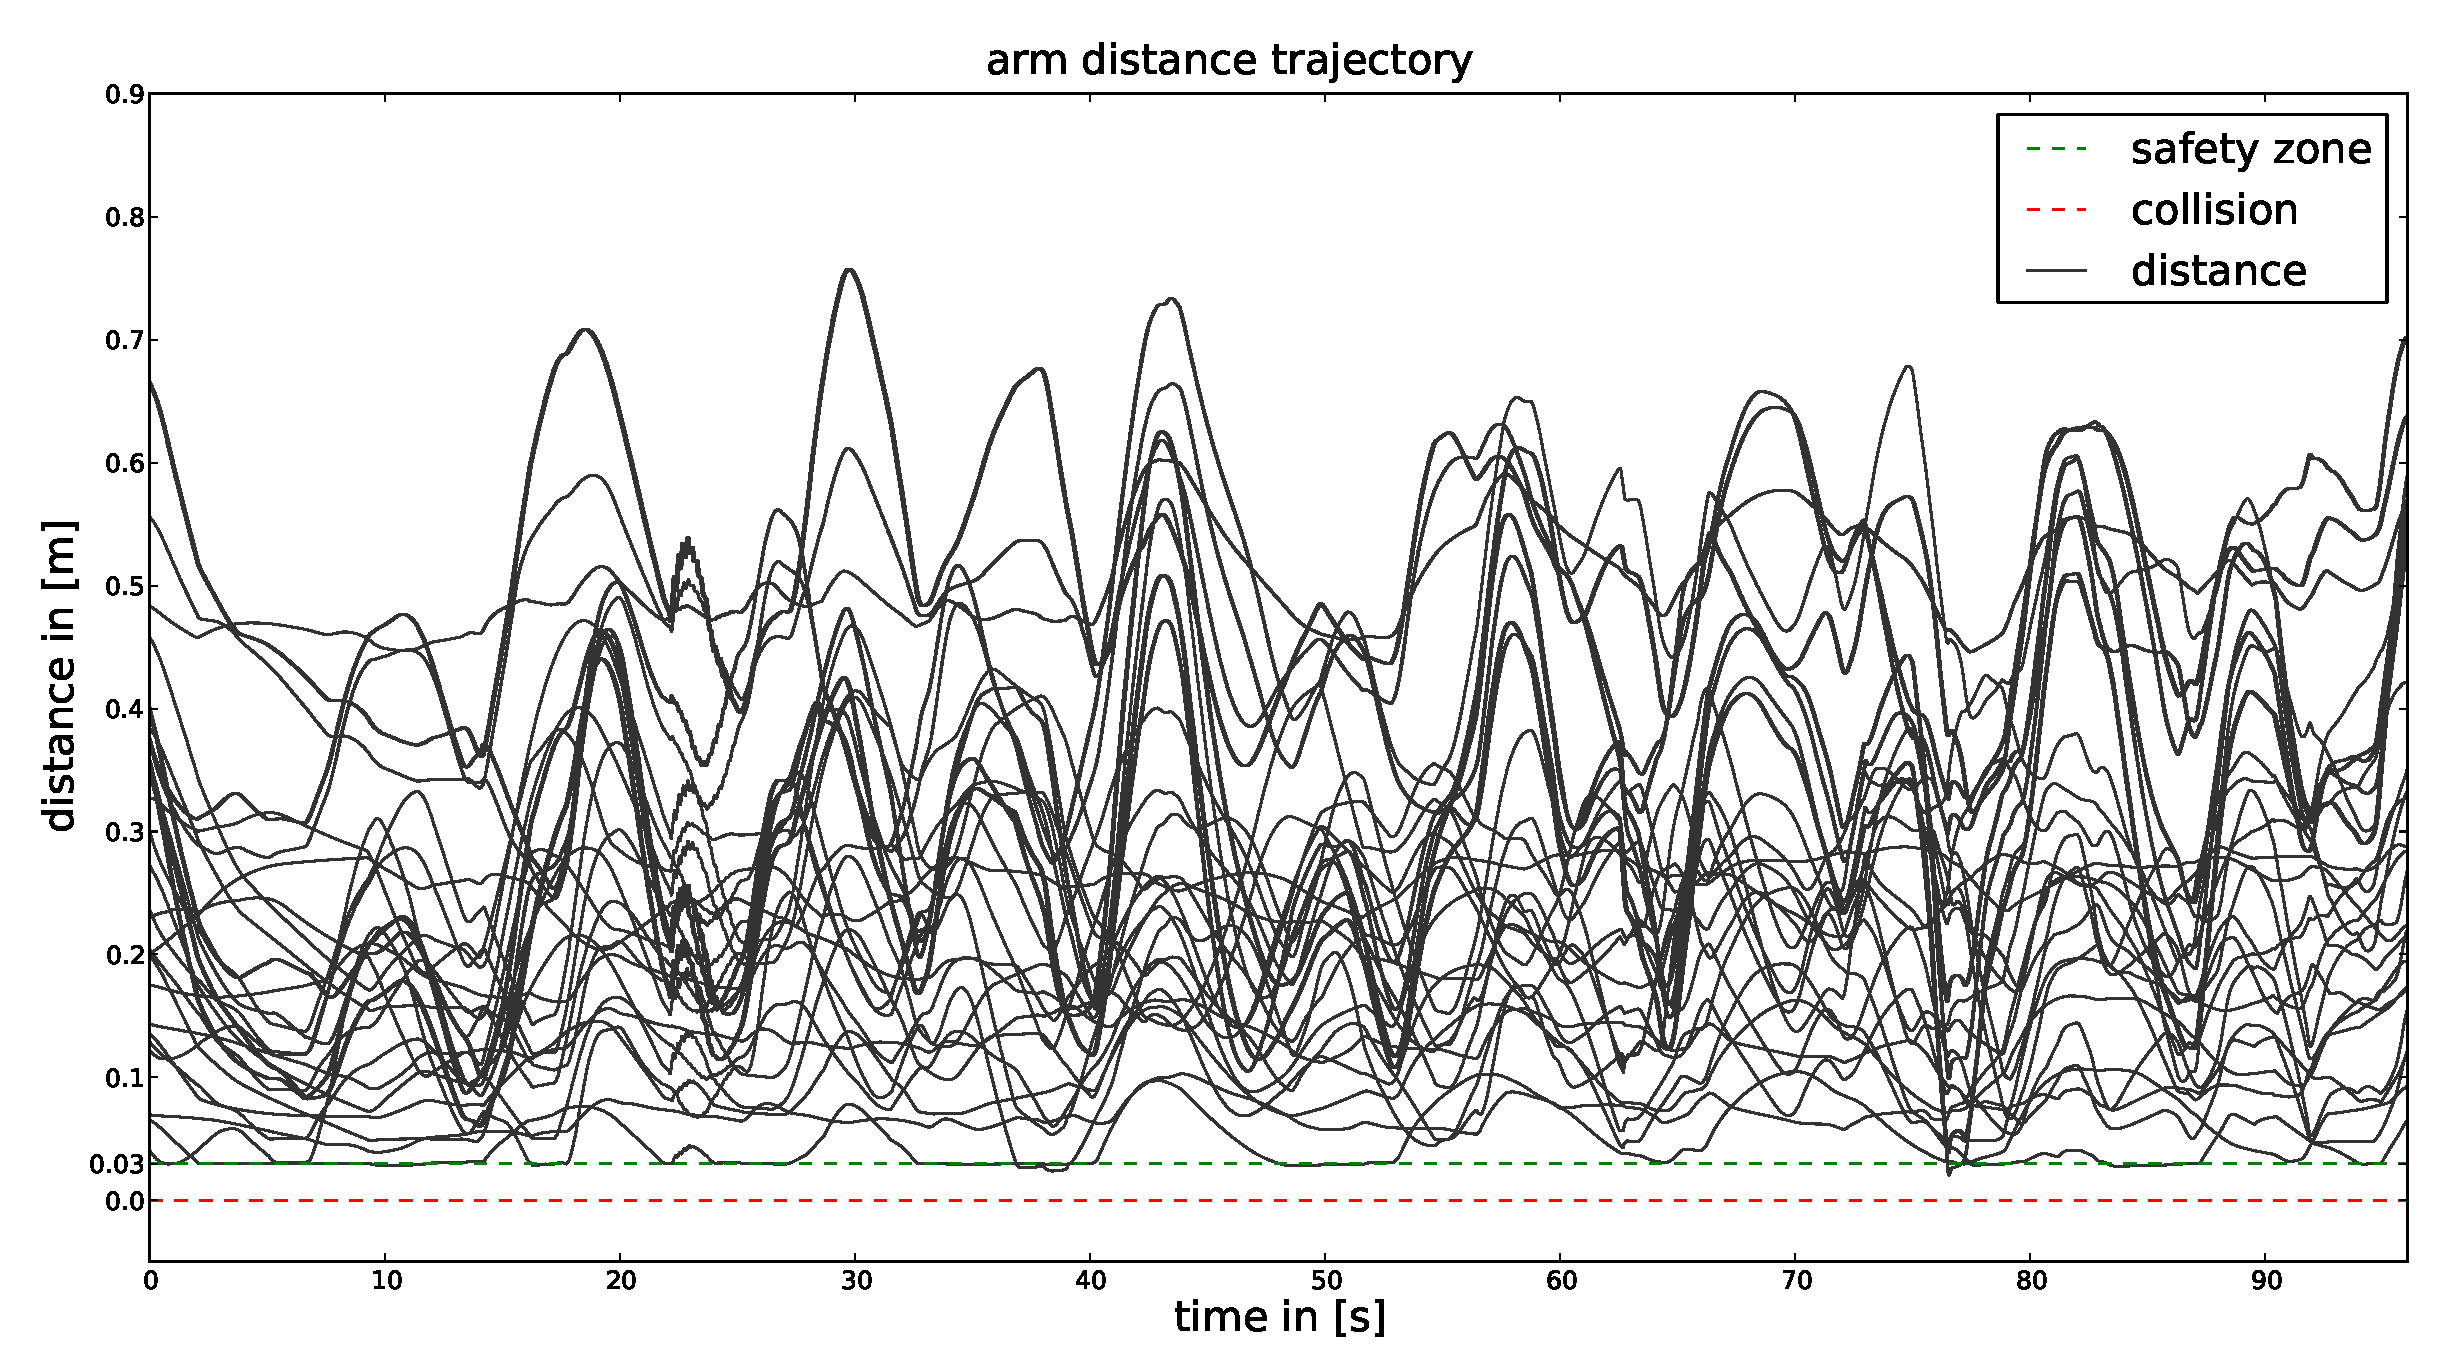
\includegraphics[width=\textwidth]{../figures/full/distance.eps}
    \caption{Distance plot of randomly changed trajectory of both arms. The collision avoidance takes all possible collision pairs into consideration. The result is equally satisfying as with predefined controlled movements.}
    \label{fig:selfcollisiondistancefull}
\end{figure}

\subsubsection*{Left Arm vs. Right Arm}
The result in the previous example, gave already a convincing outcome. We could assure, that all collisions (also in unexpected movements) are successfully avoided. Yet, we are mainly interested to position the hands in the most accurate way, meaning as close as possible to the desired position. Figure \ref{fig:selfcollisionfullerror} extracts exclusively the resulting euclidean error of the left and right arm. As we can easily see, the desired goal position is roughly getting reached. Obviously, the reason for this is that a collision occurs before reaching the desired goal. Thus, the hierarchy works as expected as the collision avoidance takes precedence over positioning one of the arms.  
\begin{figure}[h!]
  \centering
    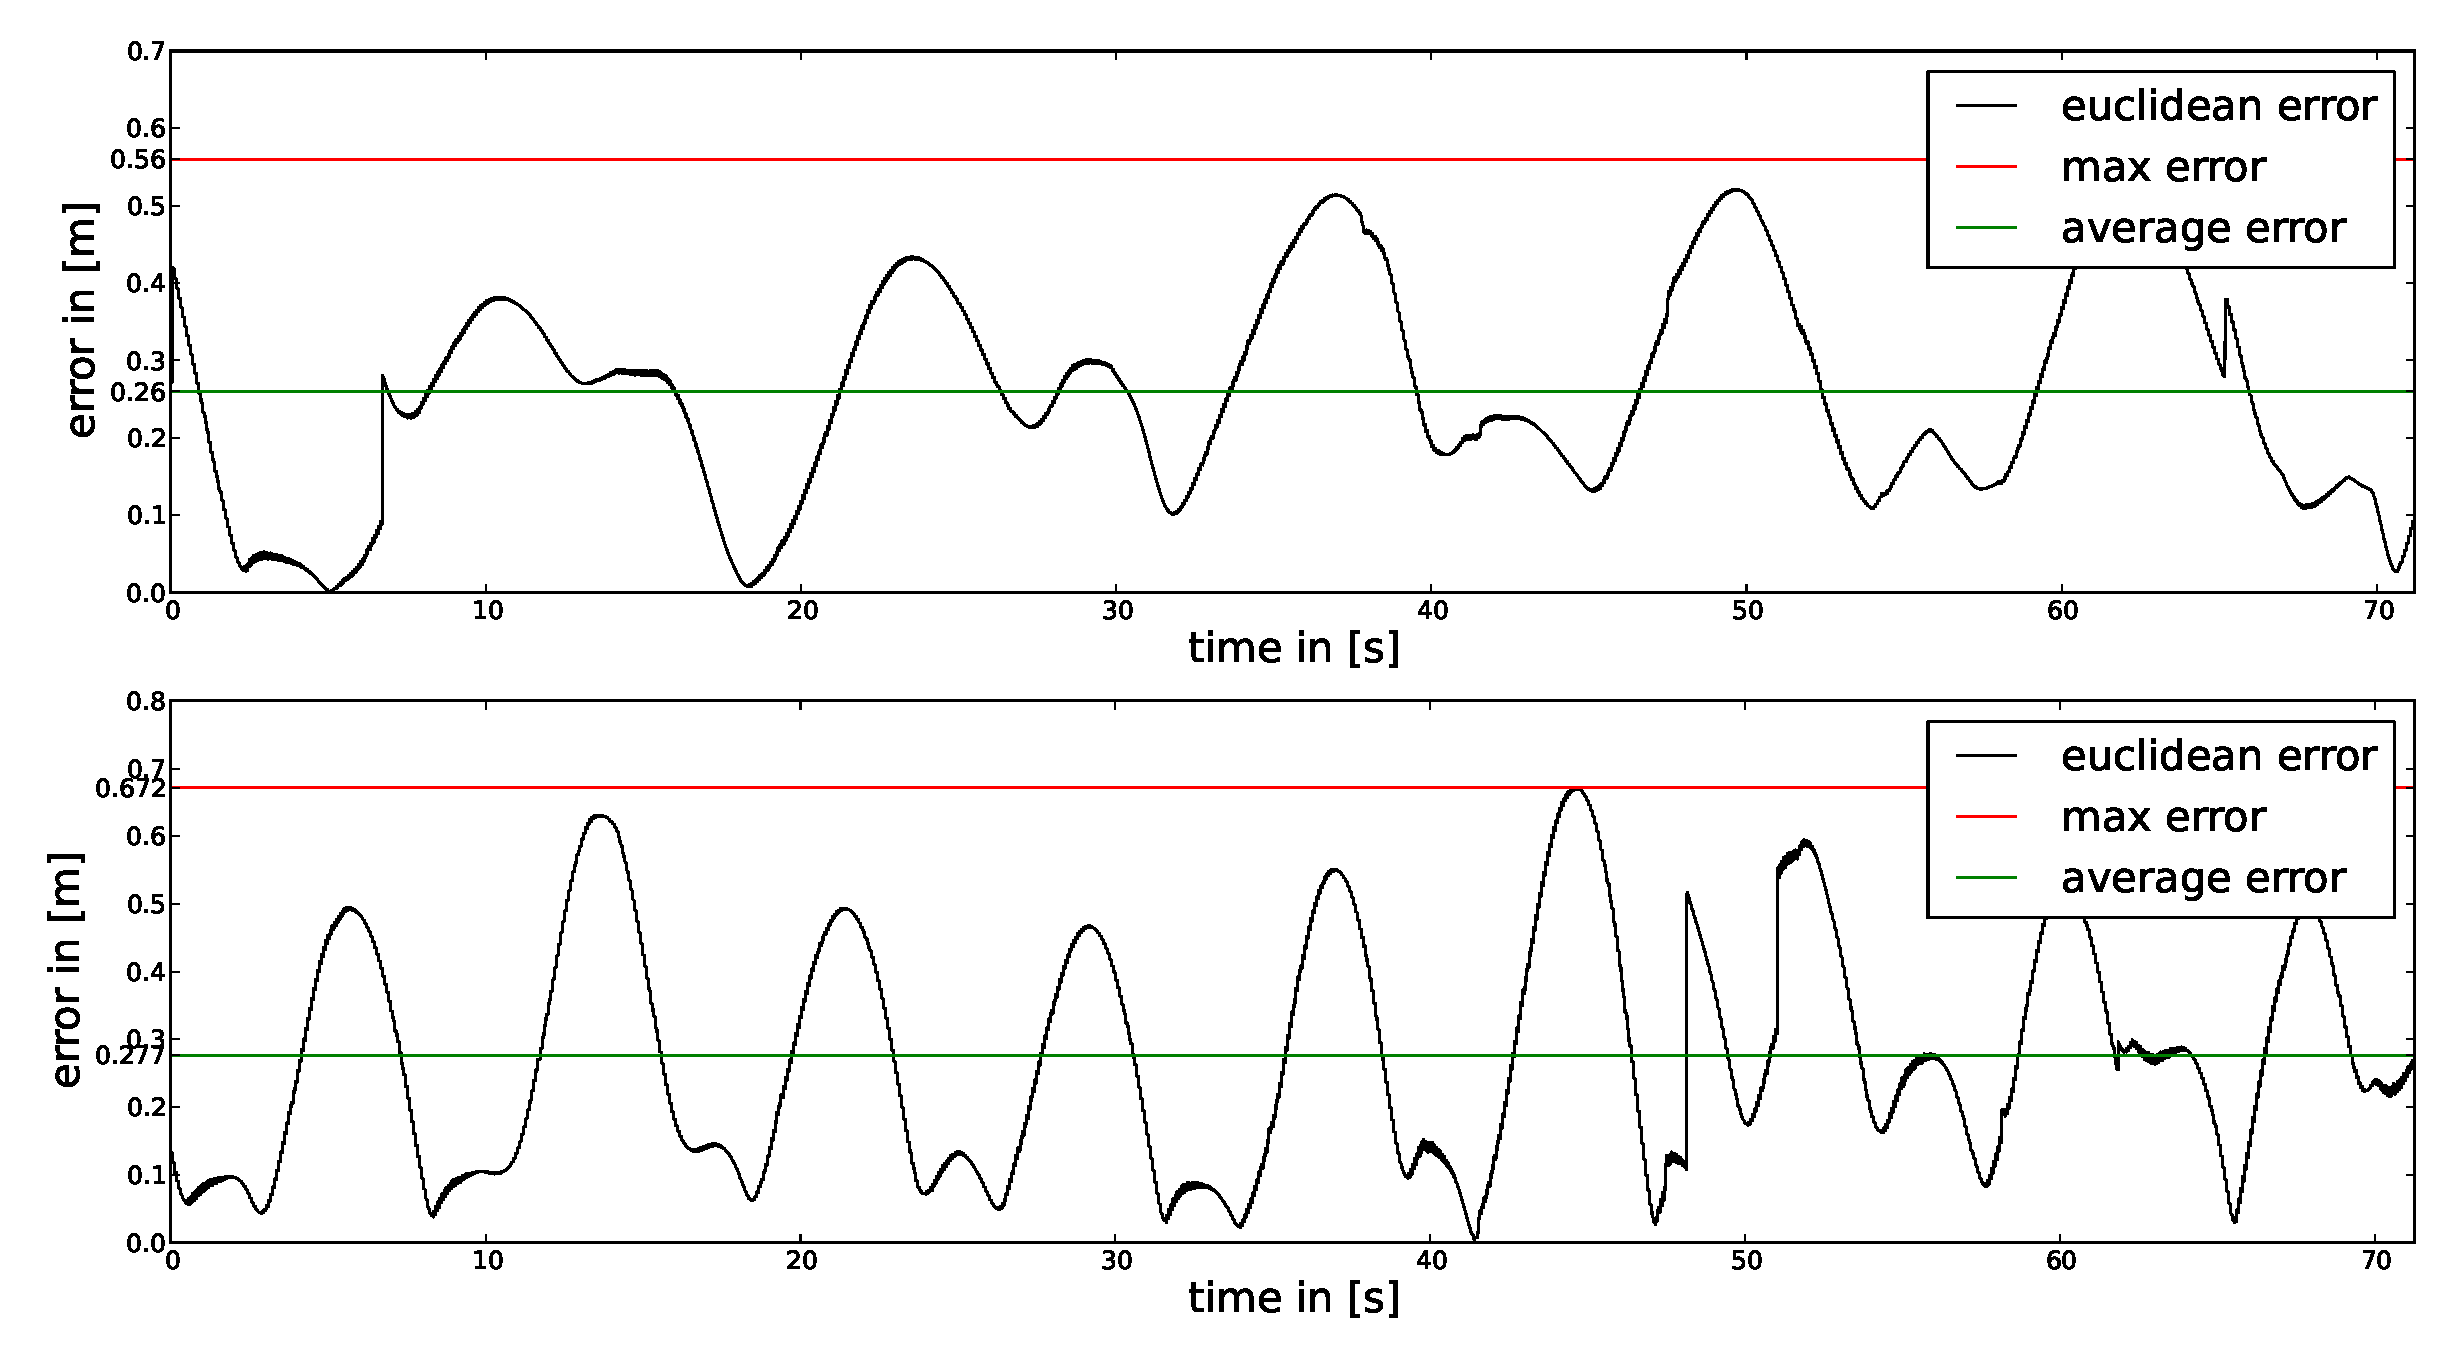
\includegraphics[width=\textwidth]{../figures/full/error.eps}
    \caption{Extraction of the emerging euclidean error. The average error is visualized in green, the maximum error value in red. We can see that both arms have a remarkable non-zero average error.}
    \label{fig:selfcollisionfullerror}
\end{figure}

Let us have a closer look at the emerging error. The key values, such as average and maximum error value are comparably listed in table \ref{tab:errors}.
\begin{table}[h!]
\centering
\begin{tabular}{c c c} 
\hline
\multicolumn{3}{ |c| }{Euclidean Error [in m]} \\
\hline
\textbf{side} & \textbf{average} & \textbf{maximum} \\
\hline
left & 0.260 & 0.560 \\[0.2em]
\hline
right & 0.277 & 0.672 \\
\end{tabular}
\caption{error value extraction of plot displayed in figure \ref{fig:selfcollisionfullerror}}
\label{tab:errors}
\end{table}
Considering those values in the above table raises immediately the question about the hierarchy of the two low prioritized positioning tasks. For the above experiment, the left arm was placed over the right arm. Thus, the printed values are going along with this, yet probably not as meaningful as hoped.

To examine the priority conditions inside the hierarchy, we further test exclusively the avoidance between the two arms against each other. To do so, we define a counter directional trajectory in $Y$ for the two arms. We examine this particular movement twice, changing the priority of the left and right arm, respectively.

Prioritizing the right arm over the left arm, yields to the resulting movement indicated in figure \ref{fig:armrightoverleft}. We can see that according to the hierarchy level, the right\footnote{be aware that right and left are seen from the robots position. Thus, the sequence of pictures is flipped.} arm  strictly encounters a smaller error compared to the left arm.
\begin{figure}[h!]
  \centering
    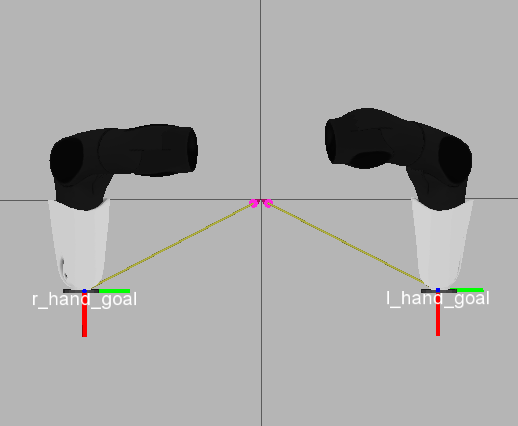
\includegraphics[width=0.23\textwidth]{../figures/right_over_left/1.png}
    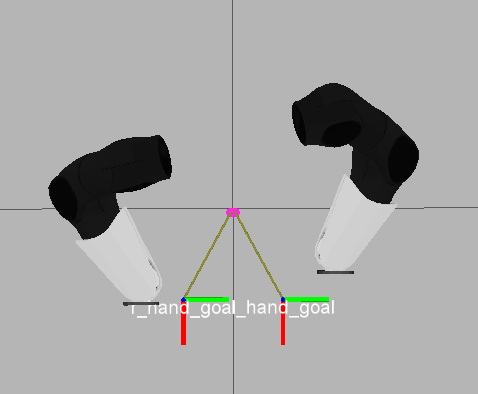
\includegraphics[width=0.23\textwidth]{../figures/right_over_left/2.png}
    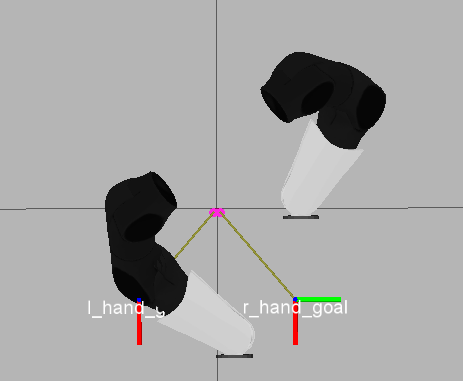
\includegraphics[width=0.23\textwidth]{../figures/right_over_left/3.png}
    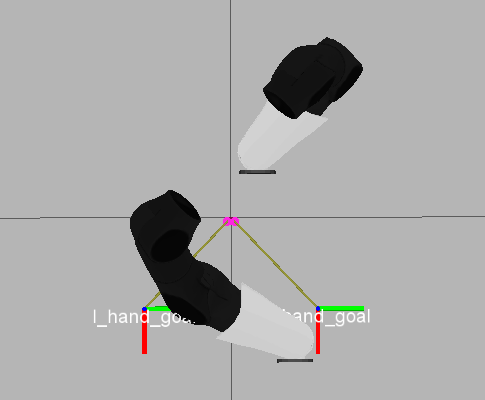
\includegraphics[width=0.23\textwidth]{../figures/right_over_left/4.png}
    \caption{Collision avoidance between both arms. The right arm takes precedence over the left arm.}
    \label{fig:armrightoverleft}
\end{figure}

Equally, we examined the inverse setup, having the left arm taking a higher priority than the right arm. Also, we display the sequence of movement in figure \ref{fig:armleftoverright}. As expected, the solution is exactly mirrored. The left arm describes a smaller error due to the higher priority.
\begin{figure}[h!]
  \centering
    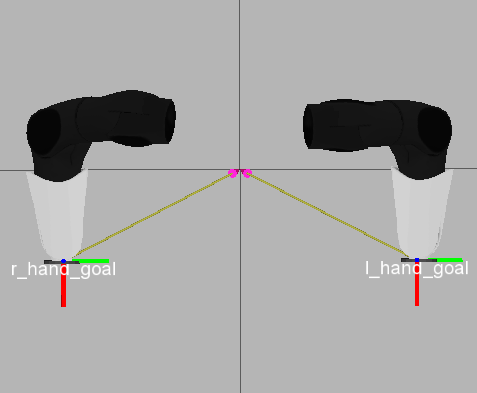
\includegraphics[width=0.23\textwidth]{../figures/left_over_right/1.png}
    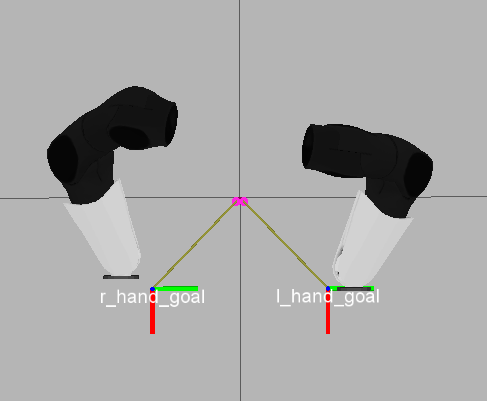
\includegraphics[width=0.23\textwidth]{../figures/left_over_right/2.png}
    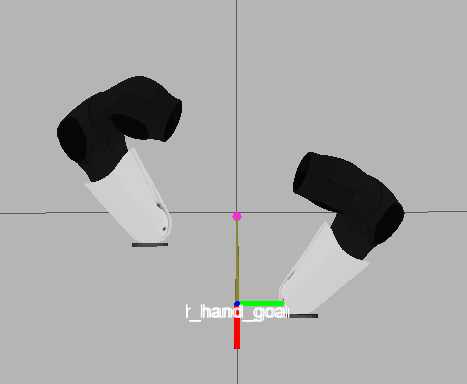
\includegraphics[width=0.23\textwidth]{../figures/left_over_right/3.png}
    \includegraphics[width=0.23\textwidth]{../figures/left_over_right/4.png}
    \caption{Collision avoidance between both arms. The left arm takes precedence over the right arm.}
    \label{fig:armleftoverright}
\end{figure}

The actual remarkable outcome of this experiment is the fact that the higher priority task encounters a deviation of its desired position, although having precedence over the respective other one. In the latter, we will suggest to name this behavior \textit{Inversion of Hierarchy}. The synchronous collision avoidance influences the underlying tasks in a counter intuitive way, hence the name. As we can see in both displayed movements, the lower prioritized arm tries to avoid the higher prioritized arm to its best solution. At the same time though, the proximity between both arm rises until the lower priority encounters a clamping situation with zero velocity. This situation is equal to the distance violation we saw during the external collision avoidance tests. On the same hand, the higher prioritized arm still has to avoid every self-collision. For this reason, it also has to leave its desired position to keep the required distance threshold. Again, we refer to the next chapter \ref{sec:results}, where we verbosely analyze this outcome and provide mathematical reasoning.

\section{Results \& Discussion}\label{sec:results}

The overall outcome of the conducted experiments above is satisfying. We can see that, the applied method of decomposing the robots collision model into capsules yields to a smooth trajectory. Since we run those algorithms successful on the robot with $100Hz$, we can state, that the implementation is reasonably efficient. Moreover, we do not encounter any shaking of the robot body parts, even with a decent execution speed. With respect to the examined self-collision tests, we can also see a successful coverage of the complete body. Based on the placed capsules, the applied safety zone provides enough margin to bridge the transition between two adjacent capsules. 

For the collision avoidance, we firstly tested our introduced method against external collision objects. External objects get strictly avoided with a continuous and optimal displacement of the actuated body part as long as this has an initial and non-zero velocity. In case of an static actuated body part with zero velocity, we have to find a reasonable trade-off between oscillating and allowed violation of the specified safety zone. 

The self-collision avoidance represents the same task definition as for avoiding external objects, yet in a larger scale. For this, we configure the velocity damping task to avoid any collision with other body parts instead of one external object. This changes the task definition not to define one constraint inside the hierarchical solver but $\frac{1}{2}n^2$, where $n$ denotes the number of entries inside the collision matrix for all capsules. Since we run the self-collision avoidance in a one-directional manner, we only consider the upper triangle of this collision matrix, hence the division by 2. 

We state that all self-collisions can be avoided with great success. We encountered, besides a neglect able numerical error, that a collision avoidance based on closest point pairs of capsules yields to no self-collision. Equally important, we could execute the full collision matrix and additional lower prioritized tasks for positioning the end-effectors of both arms still in a decent speed. This generally justifies the application of this method to be sufficient enough to avoid (self-)collisions. On the same hand, it provides enough DOF to operate both arms in a reasonable speed and workspace.

\subsection{Violations of Safety Distance}
The above presented experiments show great success and give positive results for preventing self-collisions. Yet, we encountered that in certain cases, the safety zone gets violated. This misbehavior has the most impact, when the actuated body part is on a fixed position. In case of a moving collision object, the robot does not possess enough initial velocity to avoid the object in time. We similarly run into the same behavior for the self-collision avoidance, whenever clamping situations occur, which forces certain body parts to slow done until almost no velocity. 

The reason for this violation comes from the fact, that the applied method for avoiding collisions does not generate any velocity. In contrast to other popular methods such as repulsive forces, we produce no force rather than restricting the existing velocity not to proceed any further in the direction of possible collisions. For convenience, we present the velocity damping formulation of \ref{eqn:taskdampconstraint} again:
\begin{equation}\label{eqn:extaskdamping}
\vec{n}^T\vec{J(p,q)} \vec{\dot{q}} \geq - \epsilon \frac{d - d_s}{\Delta t} 
\end{equation}
A static position of the end-effector results in $\vec{\dot{q}} = 0$. The above formulation \ref{eqn:extaskdamping} thus turns into equation \ref{eqn:extaskdampingzero}, which is mathematically satisfied until $d_s$ reaches $d$. 
\begin{equation}\label{eqn:extaskdampingzero}
0 \geq - \epsilon \frac{d - ds}{\Delta t} 
\end{equation}
In the next step, $d_s$ becomes smaller than $d$, which implies an error calculation. Thus, the right hand side of the inequality in \ref{eqn:extaskdampinginverse} turns into a positive expression as $d - d_s$ becomes negative. At the same hand, the directional vector $n$ points now outside of the collision center. The overall expression flips the sign, so the inequality, which becomes finally:
\begin{equation}\label{eqn:extaskdampinginverse}
\vec{n}^T\vec{J(p,q)} \vec{\dot{q}} \leq  \epsilon \frac{\mathit{distance}}{\Delta t} 
\end{equation}
Note, that $distance$ here implies a negative value, since $d-d_s$ denotes a negative value here. This case actively produces a positive $\vec{\dot{q}}$ and the actuated end-effector moves. However, this heavily depends on the amplifier $\epsilon$. 
This being said, a velocity exists when there is an positive error between the desired and the actual position. A small $\epsilon$ just slightly amplifies the existing distance violation. Thus, a rather fast moving obstacle completely overruns the arm as shown in \ref{fig:objmovesdistancek1}, because the generated velocity is simply too small. 
On the contrary, a heavy amplification of epsilon might catapult the actuated arm far outside of the damping constraint. This deactivated the damping inside the solver and the underlying positioning task tries to minimize the displacement error. Thus, the robot moves again towards to collision center. This finally yields to heavy oscillations between the positioning task and velocity damping.


\subsection{Inversion of Hierarchy}
Situations which occur as in the experiment of colliding two arms show that the collision avoidance has a tremendous influence on the beneath placed and thus lower prioritized tasks against each other. As we can see in figures \ref{fig:armrightoverleft} and \ref{fig:armleftoverright}, the higher prioritized arm still encounters an error in position. Concretely explained on the example, where the right arm takes precedence over the left arm: When both arms come closer, the left arm navigates towards the torso. This movement will eventually result in a clamping situation, because of the possible collisions with the right arm. Clamping situations imply again a zero velocity. We call this behavior \textit{Inversion of Hierarchy}, since the lower priority positioning task has an remarkable impact on the above placed task. 

We could see in the experiment with a full collision matrix, that those situations occur but still do not yield in a collision. To overcome this behavior, a clearly defined gain tuning has to be done for each collision pair as well as the underlying positioning tasks. At the same time, the experiments were conducted with an equally set safety zone of $0.03m$. This might lead into undesired behavior, since certain collision pairs such as the upper arm and the torso are close by construction. Therefore, we implemented the self-collision setup based on a configuration file, where for each collision pair the specific set of parameters such as $\epsilon$ and $d_s$ are declared. 
